\documentclass[Bachelor, Final, ngerman,UKenglish]{scrbook}
%------------------------------------------------------------------------------
% This file contains a skeleton thesis for
% a Physics or Astronomy Institute in the University of Bonn

% Specify the thesis type as an option: PhD, Master, Diplom, Bachelor
% Specify the thesis stage as an option: Draft (default), Submit, Final, PILibrary

% Specify the language(s) in the class and then use babel.
% If you need more than one language, give the default language last,
% e.g. ngerman,UKenglish for a thesis in British (UK) English where you want
% to be able to set the language to German for some part of it.

%------------------------------------------------------------------------------
% Pass TeX Live version to the package
% Use command pdflatex --version to find out which version you are running
% Add option backref=false when your thesis is ready to turn off back-referencing
% in your bibliography
\usepackage[texlive=2014]{ubonn-thesis}
% Adjustments to standard biblatex style
\usepackage{ubonn-biblatex}

% Glossary package
% \usepackage[acronym,toc,nosuper]{glossaries}
% TikZ packages and libraries
% \usepackage{tikz}
% \usepackage{tikz-3dplot}
% \usepackage{pgfplots}
% \usetikzlibrary{positioning,shapes,arrows}
% \usetikzlibrary{decorations.pathmorphing}
% \usetikzlibrary{decorations.markings}
\usepackage{thesis_defs}

%for tables
\usepackage{multirow}
\usepackage{feynmp-auto}

%------------------------------------------------------------------------------
% Instead of colouring  links, cites, table of contents etc.
% put them in a coloured box for the screen version.
% This is probably a good idea when you print your thesis.
% \hypersetup{colorlinks=false,
%   linkbordercolor=blue,citebordercolor=magenta,urlbordercolor=darkgreen
% }

%------------------------------------------------------------------------------
% When writing your thesis it is often helpful to have the date and
% time in the output file. Comment this out for the final version.
%\ifoot[\today{} \thistime]{\today{} \thistime}

% In order to check if your labels are referenced try the refcheck package
% \usepackage{refcheck}

%------------------------------------------------------------------------------
% biblatex is included by ubonn-thesis. Look there for the settings used.
% See the options for settings that can be changed easily.
% For further changes copy the \RequirePackage[...]{biblatex} here
% and include ubonn-thesis with the option biblatex=false.

% Specify the bibliography files here and not at the end!
% Use standard_refs-bibtex if you use bibtex or bibtex8
% and standard_refs-biber  if you use biber
\addbibresource{thesis_refs.bib}
\addbibresource{../refs/standard_refs-biber.bib}

%------------------------------------------------------------------------------
% The following definitions are used to produce the title pages
% needed at various stages
\newcommand{\thesistitle}{Development of a Particle Flow framework for Run 2 data and data-MC comparison}
\newcommand*{\thesisauthor}{Christian Kirfel}
\newcommand*{\thesistown}{Place of birth}
\renewcommand*{\InstituteName}{\PI}
\renewcommand*{\inInstitute}{\inPI}
\renewcommand*{\InstituteAddress}{\PIaddress}
% Adjust \thesisreferee...text depending on male/female referee
\newcommand*{\thesisrefereeonetext}{1.\ Gutachter}
\newcommand*{\thesisrefereeone}{Prof.\ Dr.\ Ian C. Brock}
\newcommand*{\thesisrefereetwotext}{2.\ Gutachterin}
\newcommand*{\thesisrefereetwo}{ Dr.\ Regina Moles-Valls}
% Date when thesis was submitted (Master/Diplom)
% Year or Month, Year when thesis was submitted (PhD)
\newcommand*{\thesissubmit}{XX.YY.2016}
% \newcommand*{\thesissubmit}{Month 2016}
% Date of thesis examination (PhD)
\newcommand*{\thesispromotion}{XX.YY.2016}
% Month and year of the final printed version of the thesis
\newcommand*{\thesismonth}{November}
\newcommand*{\thesisyear}{2016}
\newcommand*{\thesisnumber}{BONN-IR-2016-XXX}

%------------------------------------------------------------------------------
% The abstract is only needed for the printed version and should be in
% English regardless of the language of the thesis
\newcommand{\thesisabstract}{%
  \begin{otherlanguage}{UKenglish}
    This is your thesis abstract. It may be in a language that is
    different from the rest of your thesis.
  \end{otherlanguage}
}

%------------------------------------------------------------------------------
% \includeonly can be used to select which chapters you want to process
% A simple \include command just inserts a \clearpage before and after the file
% Note that \includeonly can be quite picky! Do not forget to put a
% comma after the filename, otherwise it will simply be ignored!
% \includeonly{%
%   thesis_intro,
%   thesis_appendix,
%   thesis_acknowledge
% }

%------------------------------------------------------------------------------
% Give a list of directories where figures can be found. Do not leave
% any spaces in the list and end the directory name with a /
%\captionsetup[subfigure]{justification=justified,singlelinecheck=false}


\graphicspath{%
  {../figs/}%
  {../figs/cover/}%
  {../figs/graphics/}%
  {../feynmf/}%
  {/graphics/}
}

%------------------------------------------------------------------------------
% Make a glossary and a list of acronyms
% \makeglossaries

% Glossary entries
% \input{thesis_glossary}

% Draft version - add the word DRAFT on the cover pages
\ifthenelse{\equal{\ThesisVersion}{Draft}}{%
  \usepackage{background}
  \ifthenelse{\texlive < 2013}{%
    \SetBgContents{DRAFT}
    \SetBgColor{blue!30}
  }{%
    \backgroundsetup{contents=DRAFT, color=blue!30}
  }
}

%------------------------------------------------------------------------------
\begin{document}

% Cover page of thesis - this is only needed for the printed final
% version to be submitted to the department library
% Do not use this page for thesis submission to the Prüfungsamt or Promotionsbüro!
\ifthenelse{\equal{\ThesisVersion}{PILibrary}}{%
  \typeout{Document \jobname, Info: PI library version of thesis}
  \input{../cover/\ThesisType_Cover}
}{}

% Start counting pages from the title page
\frontmatter
% Dedication has to come before \maketitle
% \dedication{For ...}



% Select the correct title page(s)
\ifthenelse{\equal{\ThesisType}{Unknown}}{%
  \typeout{Document \jobname, Error: Unknown thesis type - no title page printed}
}{%
  % Bachelor thesis only has one title page
  \ifthenelse{\equal{\ThesisType}{Bachelor}}{%
    \typeout{Document \jobname, Info: Bachelor thesis}
    \input{../cover/\ThesisType_Title}
  }{%
    \ifthenelse{\equal{\ThesisVersion}{Final} \OR \equal{\ThesisVersion}{PILibrary}}{%
      % Final and PI library versions
      \typeout{Document \jobname, Info: Final version of a \ThesisType  thesis}
      \input{../cover/\ThesisType_Final_Title}
    }{% Submission and draft versions
      \input{../cover/\ThesisType_Submit_Title}
      \typeout{Document \jobname, Info: Draft/submission version of a \ThesisType  thesis}
    }
  }
}



\pagestyle{scrplain}



%------------------------------------------------------------------------------
% You can add your acknowledgements here - don't forget to also add
% them to \includeonly above
%%------------------------------------------------------------------------------
\chapter*{Acknowledgements}
\label{sec:ack}
%------------------------------------------------------------------------------

I would like to thank ...

You should probably use \texttt{\textbackslash chapter*} for
acknowledgements at the beginning of a thesis and
\texttt{\textbackslash chapter} for the end.

%%% Local Variables: 
%%% mode: latex
%%% TeX-master: "../mythesis"
%%% End: 


\tableofcontents

\mainmatter
\pagestyle{scrheadings}

% Turn off DRAFT for the following pages
\ifthenelse{\equal{\ThesisVersion}{Draft}}{%
  \ifthenelse{\texlive < 2013}{%
    \SetBgContents{}
  }{%
    \backgroundsetup{contents={}}
  }
}{}

%------------------------------------------------------------------------------
% Add your chapters here - don't forget to also add them to \includeonly above
%==============================================================================
\chapter{Introduction}
\label{sec:intro}
%==============================================================================

The Large Hadron Collider (LHC) is an accelerator at CERN near Geneva. One of its main experiments is the general-purpose detector ATLAS. This thesis describes the performance of a reconstruction algorithm named Particle Flow.


The Particle Flow jets have recently been stabilised as one of the official jet collections to be used in the ATLAS analysis. Particle Flow combines tracker and calorimeter information and previous studies\cite{pflow16} have demonstrated that it is a promising approach improving the angular resolution and transversal momentum resolution especially for lower transversal momentum. The aim of this thesis was to create a framework for the study of Particle Flow performance on 2016 \SI{13}{\TeV} data and to perform data-Monte Carlo comparison.

This thesis is structured as follows:

Chapter 2 gives a brief introduction to the standard model of particle physics, that describes the fundamental particles and their interactions. Furthermore the chapter includes a simple description of the ATLAS detector and a more detailed explanation of tracking detectors and calorimeters since they are important for Particle Flow.

The third chapter describes the Particle Flow algorithm in detail and also presents a brief overview of the Run 1 results as well as the changes that have been applied to the algorithm for Run 2.

Chapter four summarizes the analysis framework that has been developed during this thesis. It gives an explanation for all the important tools used in the framework and concludes by listing the tools that still have to be implemented or generated for Particle Flow.

Chapter 5 then finally presents the results derived from data/Monte Carlo comparison for 2016 data on $Z\rightarrow \mu \bar{\mu}$ events.




%%% Local Variables: 
%%% mode: latex
%%% TeX-master: "../mythesis"
%%% End: 


\chapter{Theoretical and experimental basics}
\label{theory}

\section{The Standard Model of Particle Physics}

The Standard Model of particle physics summarizes the current knowledge of fundamental particles and their interactions. The model applies to scales of 1 fm and below. Gravity, being the fourth fundamental force is not included as it is negligible for most phenomena at this scale.

The current view is that all matter is made out of three kinds of elementary particle being leptons quarks and mediators.
There are six leptons falling into three families according to their charge, electron number, muon number and tau number. 

Similiar to that there are six flavors of quarks separated by strangeness (S), charm (C), beauty (B), and truth (T). As the leptons the quarks fall into three generations.
For both kinds of particles the mass rises with the generations and each generation comes as a doublet. The first particle of each lepton doublet is uncharged and referred to as a neutrino while the second particle has charge \num{-1}.
For each quark doublet there is an element with fractional charge $-\frac{1}{3}$ and an element with fractional charge $\frac{2}{3}$.
To each of these particles exists an anti particle of opposite charge.

The third kind of particle included in the standard model is the mediator. Mediators are gauge bosons the exchange of which allows the particles to interact. There are four kinds of elemtary interactions of which the strong electromagnetic and weak interaction are included in the model. The fourth interaction is the gravitational force.
The gauge particles for the strong interaction are the gluons carrying colour charge, the electromagnetic mediator is the photon ($\gamma$) and the weak mediators are the $W^{\pm}$ and $Z$ bosons.
Tables \ref{lepton properties}, \ref{quark properties} and \ref{mediator properties} summarize the particles and their pivotal properties.
\newpage


\begin{table}[h]
\centering
\renewcommand{\arraystretch}{1.2}
\begin{tabular}{l|l|S|S|S|S|}
\cline{2-6}
                                   & symbol        & \text{Charge}  & \text{\ensuremath{L_e}} & \text{\ensuremath{L_{\mu}}} & \text{\ensuremath{L_{\tau}}} \\ \cline{2-6} 
\multirow{2}{*}{First generation\{}  & $e$             & -1       & 1    & 0          & 0           \\ \cline{2-6} 
                                   & $\nu_e$        & 0        & 1    & 0          & 0           \\ \cline{2-6} 
\multirow{2}{*}{Second generation\{} & $\mu$           & -1       & 0    & 1          & 0           \\ \cline{2-6} 
                                   & $\nu_{\mu}$  & 0        & 0    & 1          & 0           \\ \cline{2-6} 
\multirow{2}{*}{Third generation\{}  & $\tau$          & -1       & 0    & 0          & 1           \\ \cline{2-6} 
                                   & $\nu_{\tau}$ & 0        & 0    & 0          & 1           \\ \cline{2-6} 
\end{tabular}
\caption{Lepton properties}
\label{lepton properties}
\end{table}

\begin{table}[h]
\centering
\renewcommand{\arraystretch}{1.2}
\begin{tabular}{l|l|S|S|l|l|l|l|l|l|}
\cline{2-10}
                                      & Symbol & \text{Charge Q}      & \text{mass [GeV]}       & D  & U & S  & C & B  & T \\ \cline{2-10} 
\multirow{2}{*}{First generation \{}  & $d$    &\text{\ensuremath{-\frac{1}{3}}} & 4.8   & -1 & 0 & 0  & 0 & 0  & 0 \\ \cline{2-10} 
                                      & $u$    & \text{\ensuremath{\frac{2}{3}}}  & 2.3   & 0  & 1 & 0  & 0 & 0  & 0 \\ \cline{2-10} 
\multirow{2}{*}{Second generation \{} & $s$    & \text{\ensuremath{-\frac{1}{3}}} & 95    & 0  & 0 & -1 & 0 & 0  & 0 \\ \cline{2-10} 
                                      & $c$    & \text{\ensuremath{\frac{2}{3}}}  & 1275   & 0  & 0 & 0  & 1 & 0  & 0 \\ \cline{2-10} 
\multirow{2}{*}{Third generation \{}  & $b$    & \text{\ensuremath{-\frac{1}{3}}} & 4180   & 0  & 0 & 0  & 0 & -1 & 0 \\ \cline{2-10} 
                                      & $t$    & \text{\ensuremath{\frac{2}{3}}}  & 173210 & 0  & 0 & 0  & 0 & 0  & 1 \\ \cline{2-10} 
\end{tabular}
\caption{Quark properties}
\label{quark properties}
\end{table}

\begin{table}[h]
\centering
\renewcommand{\arraystretch}{1.5}
\begin{tabular}{|l|l|l|l|l|}
\hline
Interaction     & Theory & Mediator        & Charge          & Coupling  \\ \hline
Strong          & QCD    & gluons (8)      & colour          & 1         \\ \hline
Electromagnetic & QED    & photon $\gamma$ & electric charge & $10^{-1}$ \\ \hline
Weak            & GSW    & $W^{\pm}, Z$    & weak isospin    & $20^{-6}$ \\ \hline
\end{tabular}
\caption{Mediator properties}
\label{mediator properties}
\end{table}

Given this the standard model of particle physics has been a very successful model for a very long time and still holds for most cases.
Nevertheless the model has some commonly known weaknesses and does not claim to be complete. For example the gravitational force is not included and in the standard model neutrinos are massless which would not allow the oscillations observed in neutrinos originating from the sun.
For further information check \cite{griffith08}, \cite{thomson13} and \cite{brock11}.

In 2012 the Higgs boson was discovered at the Large Hadron Collider. It is a spin-0 scalar particle with a mass of $m_H$ $=$ $\SI{125}{\GeV}$ and it represents the mechanism which gives all particles their mass.

\newpage





\section{The LHC and ATLAS}

The analysis for this thesis has been performed in the ATLAS collaboration. The ATLAS-Detector is one of the four main experiments at the LHC at CERN. This section provides a brief overview of the LHC and ATLAS detector focusing on the aspects directly relevant for Particle Flow analysis.

In addition to a brief description of the ATLAS detector a more detailed explanation of trackers and calorimeters is given since these components are directly relevant for the explanation of Particle Flow.

\subsection{The LHC}

The Large Hadron Collider ("LHC") located at the facilities of the European Organization of Nuclear Research ("CERN") close to Geneva was built to extend the frontiers of modern particle physics by delivering high luminosities and reaching unprecedented high energies. The hadronic collider has a circumference of about \SI{27}{\km} and is located on average \SI{100}{\meter} underground.\\
The LHC is designed to collide bunches of up to \num{d11} protons at a luminosity of \SI{d34}{\per\square\cm \per\s}. The beams collide at four points where the four main experiments of the LHC are located. Two of these are special-purpose detectors, namely LHCb and ALICE while the other two, ATLAS and CMS, are general-purpose detectors.
The analysis in this thesis was performed on ATLAS data.
Figure \ref{fig:LHC} shows the LHC, the four detectors and its general location.
\begin{figure}[h]
  \centering
  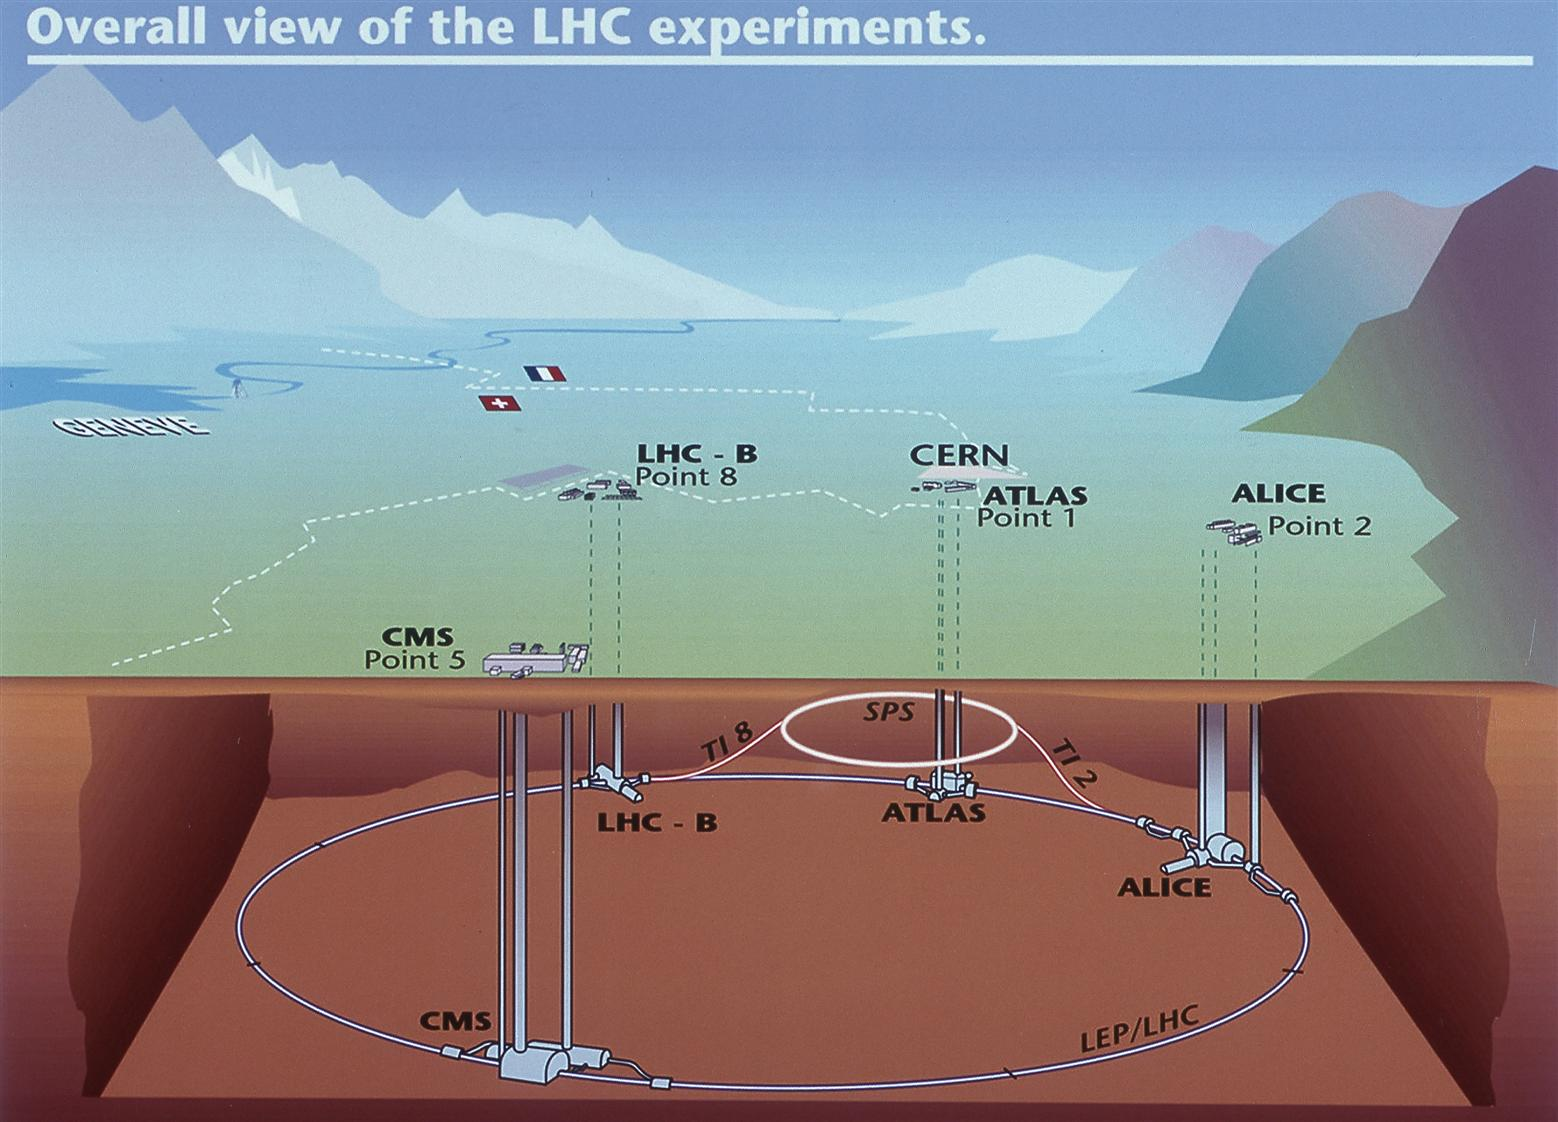
\includegraphics[width=\figwidth]{CERN-all-experiments}
  \caption[Sketch of the LHC ring, the position of the experiments and
  the surrounding countryside.]{Sketch of the LHC ring, the position
    of the experiments and the surrounding countryside. The four big
    LHC experiments are indicated(ATLAS, CMS, LHC-B and ALICE)along with their injection lines(Point 1, 2, 4, 8)\cite{atlasfigures}}
  \label{fig:LHC}
\end{figure}


\subsection{The ATLAS Detector}

The ATLAS detector was developed to study the physic processes in a broad energy range available at the LHC. This enables the observation of highly massive particles that lower energy accelerators were not able to create and that would deliver new physics theory beyond the standard model of particle physics.
It was designed to cover the maximum number of final stages being a so called general purpose-detector.
Figure \ref{fig:atlas} shows a sketch of the ATLAS detector together with a rough scale in size not only by the given dimensions on the top and left side but also by including two average sized humans close to the left muon chambers. In the following explanations of its components are given from the inside to the outside.

\begin{figure}[h]
  \centering
  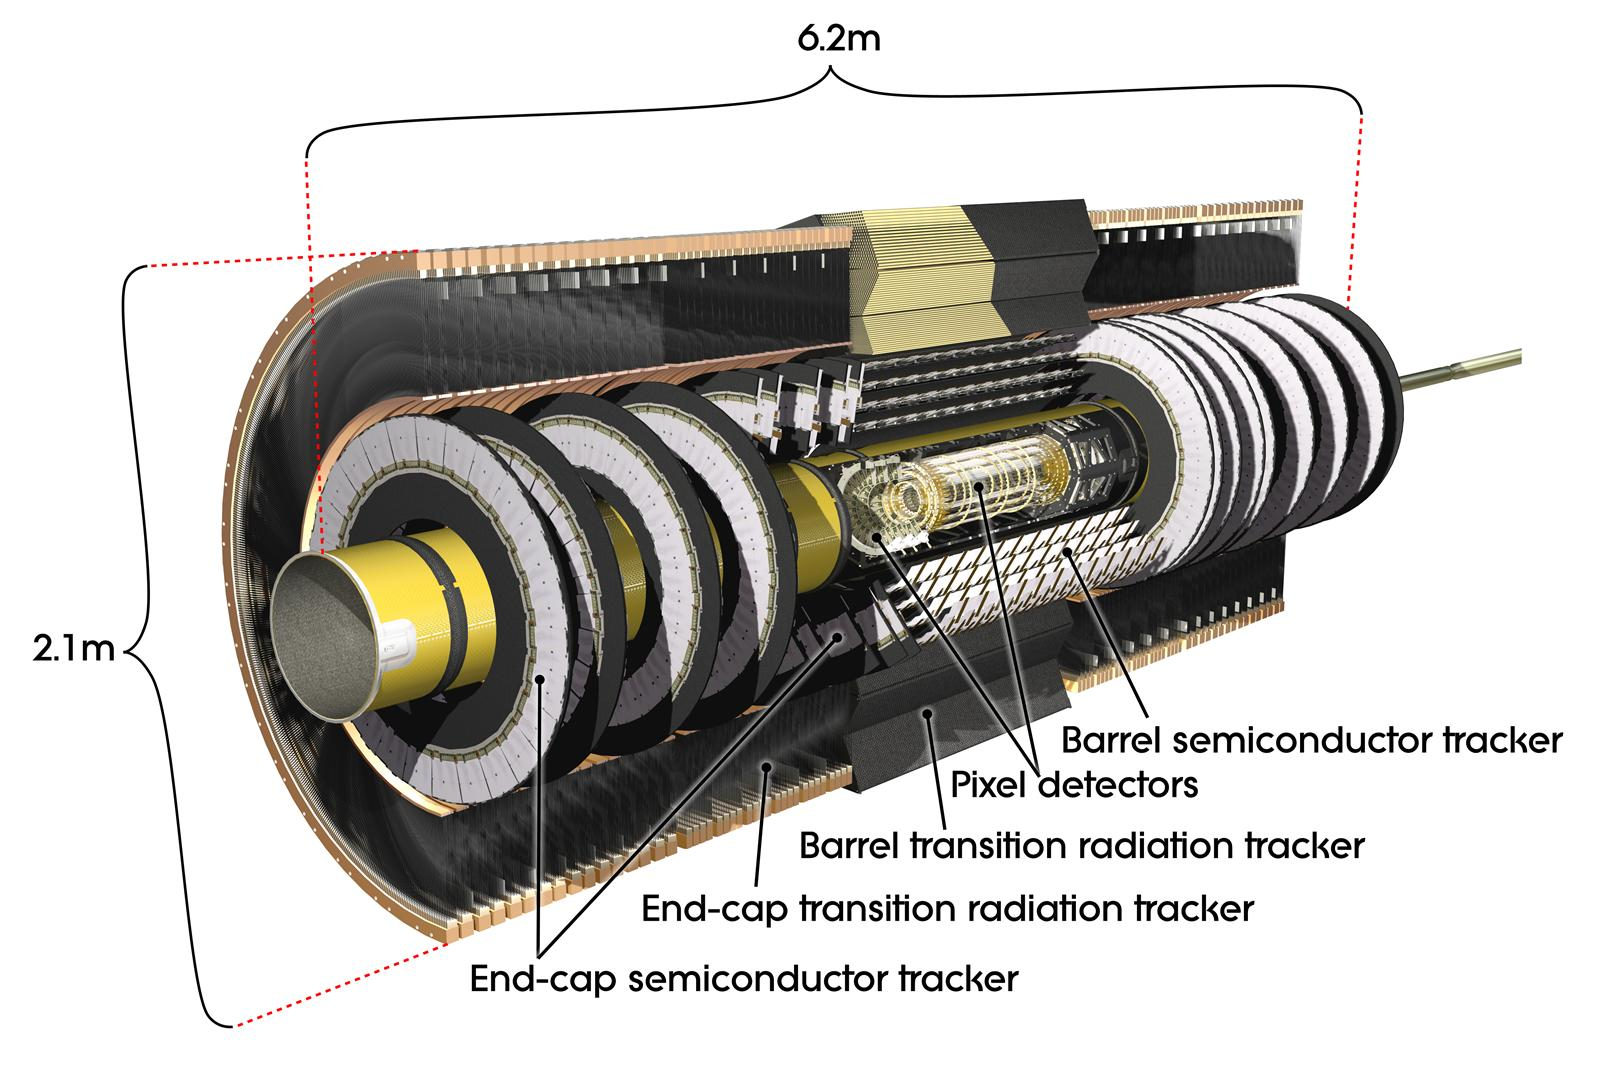
\includegraphics[width=\figwidth]{atlas-detector}
  \caption[Sketch of the ATLAS detector]{Sketch of the ATLAS detector \cite{atlasfigures}}
  \label{fig:atlas}
\end{figure}

Figure \ref{fig:atlas_sketch} shows the detector's components in a simplified way and allows to understand the importance of the order of the detector's parts. The innermost part of the detector is a tracking detector surrounded by a solenoid that creates a magnetic field to bend the charged particles' trajectory and measure their charge and momentum.
The following part of the detector is the calorimetry system. It consists of an inner electromagentic calorimeter and and outer hadronic calorimter. The outermost part is a muon spectrometer because most of the particles that cross the calorimeters undetected or do not deploy their complete energy are muons.

The detector system therefore allows to measure charge, momentum end energy of most particles.


\begin{figure}[h]
  \centering
  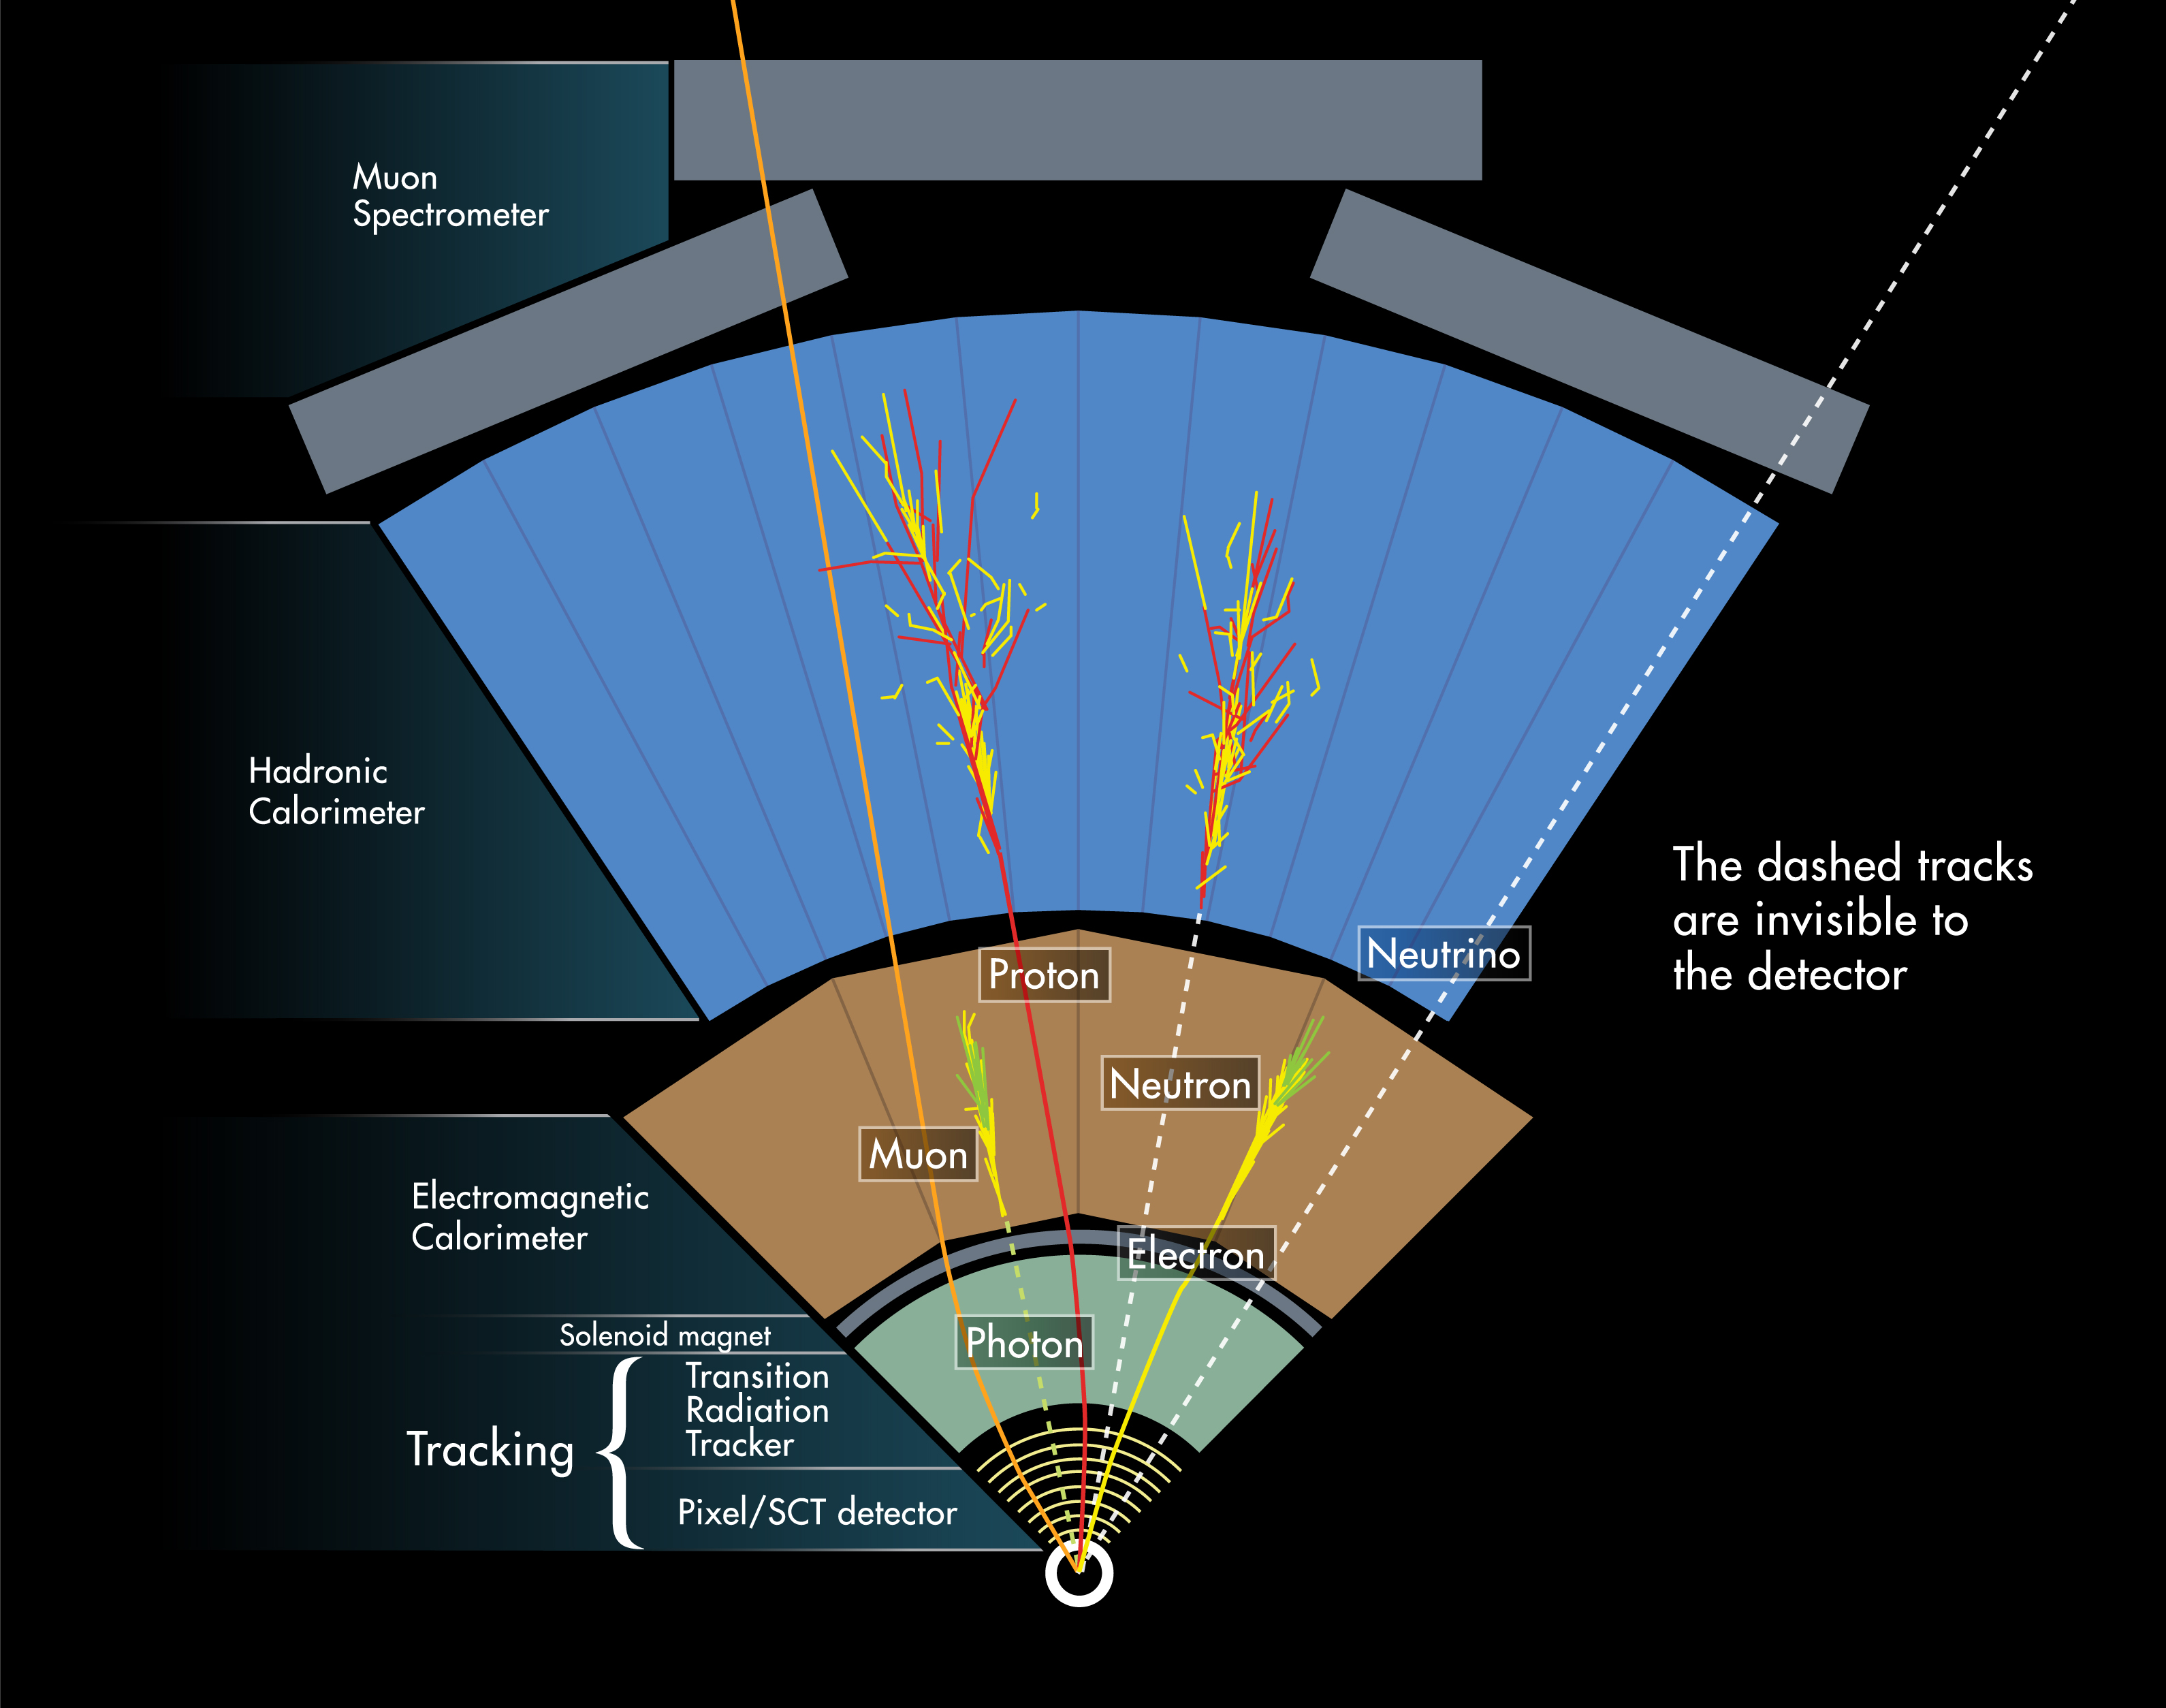
\includegraphics[width=\figwidth]{atlas-abstract}
  \caption[Sketch of the transversal section of the ATLAS detector]{Scheme of the ATLAS-detector \cite{atlasfigures}}
  \label{fig:atlas_sketch}
\end{figure}

\subsection{The ATLAS coordinate system}

The ATLAS coordinate system is defined by the beam direction with the $z$-axis pointing along the LHC's beam pipe. The corresponding transverse plane is defined by the $x$-axis pointing towards the ring's centre while the $y$-axis points upwards. The origin of the system is defined by the nominal point of interaction. The polar angle $\theta$, is the angle between the $z$-axis and the $x$-$y$-plane and the azimuthal angle $\phi$ is the angle between the $x$- and the $y$-axis.

The coordinates used in this thesis are usually the azimuthal angle $\phi$, the pseudo-rapidity $\eta$, and the transverse momentum $p_T$. The pseudo-rapidity replaces the polar angle and is defined as

\begin{equation}
\eta = \frac{1}{2} ln\left[ tan\left(\frac{\theta}{2}\right)\right].
\end{equation}

The transverse momentum is defined by

\begin{equation}
p_T = \sqrt{p_x^2 + p_y^2}
\end{equation}
where $p_x$ and $p_y$ are the momenta along the corresponding axes. 

The angular variables are defined within

\begin{equation}
\eta \in [-\infty,\infty],\,
\phi \in [-\pi,\pi].
\end{equation}
\subsection{Tracking detectors}

To measure momentum, trajectory and charge of charged particles usually tracking detectors are used.

There are two main categories of tracking detectors following the same general principle, gaseous detectors and semiconductor detectors. If ionizing radiation passes any given medium it will create electron-hole pairs. These charge carriers can then be collected by an electric field. Depending on the detector the signal caused by the charge carriers can be related to the coordinate of ionization in space and time.

\begin{itemize}
\item Gaseous detectors: Gaseous detectors are based on the greater mobility of ions and electrons in the gas. The basis of the detector is usually a chamber filled with a proper gas. The gas contains an area of wires to which a strong electric field is applied. If gas atoms get ionized the charge carriers (electrons and ions) will drift to the wires and create a detectable signal. The wires give a rough estimation of space which is normally improved by calculating the exact ionization location from the drift time.

\item Semiconductor detectors: Semiconductor detectors are as their name implies based on crystalline semiconductor material such as silicon and germanium. Their working principle is quite similar to that of gaseous detectors but the gas is exchanged by solid semiconducting material. In semiconducting material ionizing radiation will create electron-hole pairs instead of electron ion pairs that then can travel in a strong electric field to be detected. The big advantage of semiconductor detectors over gaseous detectors is that the energy required to create an electron-hole pair is about 10 times lower than the energy needed to ionize gas atoms. These detectors are commonly structured into wafers or pixels that allow a determination of the space.
\end{itemize}

Usually a magnetic field surrounds tracking detectors to bend the track and that way be able to compute the particles momentum and charge based on the curvature.


In the ATLAS detector both the inner detector and the muon spectrometer are tracking detectors.

\subsubsection{The Inner Detector}

The innermost part of the ATLAS detector is called the Inner Detector, which consists of three sub-components, the Pixel detector (Pixel), the Semi-Conductor Tracker (SCT) and a Transition Radiation Tracker (TRT). Each of these sub-detectors is divided into the so called barrel part and two end-caps. The Inner Detector covers a region of $|\eta| < \num{2.5}$ which also limits the region in which Particle Flow can be used as its highest efficiency.

\subsubsection{The Muon spectrometer}

The second tracking detector of ATLAS is the muon spectrometer which is the outermost part of the detector. The task of the spectrometer is to detect charged particles transversing the calorimeter without being stopped or deploying their complete energy, and to do both trigger and tracking to measure their momentum. Due to these two tasks the spectrometer is bifid with the first part being the trigger chamber covering a range of $|\eta|<2.4$, followed by the high-precision chamber with a range of $|\eta|<2.7$. The main detector's support feet cause a further gap at about $\phi = \ang{300}$ and $\phi = \ang{270}$. 

The high-precision detector uses monitored drift tubes (MDTs) with the exception of the innermost part of the innermost end-cap disk which utilizes Cathode Strip Chambers (CSCs). The trigger chamber uses resistive-plate chambers (RPCs) for the barrel parts and Thin-Gap Chambers (TGCs) for the end-caps. The momentum calculation is then performed by the field of the toroid magnet.



\subsection{Calorimeters}

In particle physics a calorimeter is a device to measure first and foremost the total energy of a particle. Most of the time some positional information is taken  additionally.
The idea is that most particles loose all their momentum while crossing the calorimeter. Measuring the energy deposited this way gives a value for the particle's energy.
Usually a particle deposits its energy by initiating a particle shower, the energy of which is then collected and measured.
Calorimeters are distinguished by the main interaction of the particles one aims to detect. 
\subsubsection{Electromagnetic Calorimeters}

Electromagnetic calorimeters are designed to detect charged particles that primarily via the electromagnetic interaction and to measure their total energy. Usually these particles are electrons and photons. There are various methods to construct these detectors. An example would be the usage of inorganic scintillators. These scintillators should be optically transparent and have a short radiation length to contain the shower in a compact region. The detection can then be followed by photon detectors with photo-multipliers which measure the emitted light being proportional to the detected particle's energy.

The electromagnetic calorimeter at ATLAS is a high-resolution and high-granularity liquid-argon sampling calorimeter using lead as absorber material. The calorimeter consists of two half-barrels which are only separated by a small gap at the interaction point. The endcaps at each side are segmented into two coaxial wheels to cover different polar angles.

\subsubsection{Hadronic calorimeters}

Hadronic calorimeters are used to obtain the energies of hadronic particles.
Due to the relatively large distance between interactions these calorimeters occupy a significantly large volume in the detector.

A common technique to construct these calorimeters is a sandwich-like structure of alternating layers of high density absorber material and active material. 
The absorbers are used to develop the particle showers which then hit the active material and deposit their energy there. The determination of the particle belonging to the deployed energy relies on tracker information as is sketched in figure \ref{fig:atlas_sketch}. Energy in the hadronic calorimeter without a track implies a neutral hadron, for example a neutron. A single track paired with a energy deposition means that the particle was a charged hadron like a proton and if many tracks belong to a deposition a jet has been the most likely origin of the energy deposition.


The hadronic calorimter system at ATLAS is divided into three calorimeter components. The first one is the scintillator-tile calorimter covering a region of $|\eta|<\num{1.7}$. The other two are the end-cap calorimters which use liquid argon (LAr) and cover the region of $\num{1.5}<|\eta|<\num{3.2}$.
The tile calorimeter itself is divided into a central barrel and two extended barrels (compare \ref{fig:atlas}).


For more information about the ATLAS detector see the ATLAS design report \cite{atlastdr}.



\chapter{Particle Flow Reconstruction}

One of the goals of this thesis was to check the results of Particle Flow in Run 2 data. Therefore this chapter will give an overview of the results that the new algorithm has brought for Run 1 in data MC comparison. Before showing the results this chapter gives a description of the algorithm based on the Particle Flow Paper \cite{pflow16}. Then an update on how the algorithm has evolved is given before finally a bief overview of the results is presented.

\section{The Particle Flow Algorithm}

Recently only either the Calorimeter or the tracker information was used to reconstruct Jets in ATLAS events. The Particle Flow algorithm now combines tracker and calorimeter information to achieve better resolution especially at lower energies. The main advantages of including the tracker information into reconstruction are as follows:


\begin{itemize}
\item For low energy charged particles the momentum resolution of the tracking detector is superior to the calorimeter.
\item The tracking detector is able to reconstruct soft particles, which would not pass the noise threshold of the calorimeter.
\item The ATLAS tracking detector has a superior angular resolution for single charged particles.
\item Low $p_T$ charged particles may be swept out of the cone before reaching the calorimeter by the magnetic field. The tracker information allows to cluster these particles into the jet.
\item a better vertex determination could lower the pileup-contribution.
\end{itemize}

The advantages of Particle Flow have already been shown for Run 1 data in

Figure \ref{fig:pflowflowchart} sketches the important steps of the Particle Flow algorithm. The algorithm uses clusters from the calorimeters and tracks from the tracking detectors as input information. The first step is to match a track spatially to a cluster. After a pair has been found the algorithm checks whether the particle's momentum matches the energy deposited in the cluster within the expected deviation. If the energy matches a subtraction algorithm starts deciding which cells belong to the given event. If the energy deposited in the cluster is too low the algorithm includes all other clusters in a given area and then starts the subtraction.

After the subtraction the algorithm gives information about matched clusters and trackers. Furthermore energy deposited in cells that were not subtracted can be identified as remnants. 

\begin{figure}[h]
  \centering
  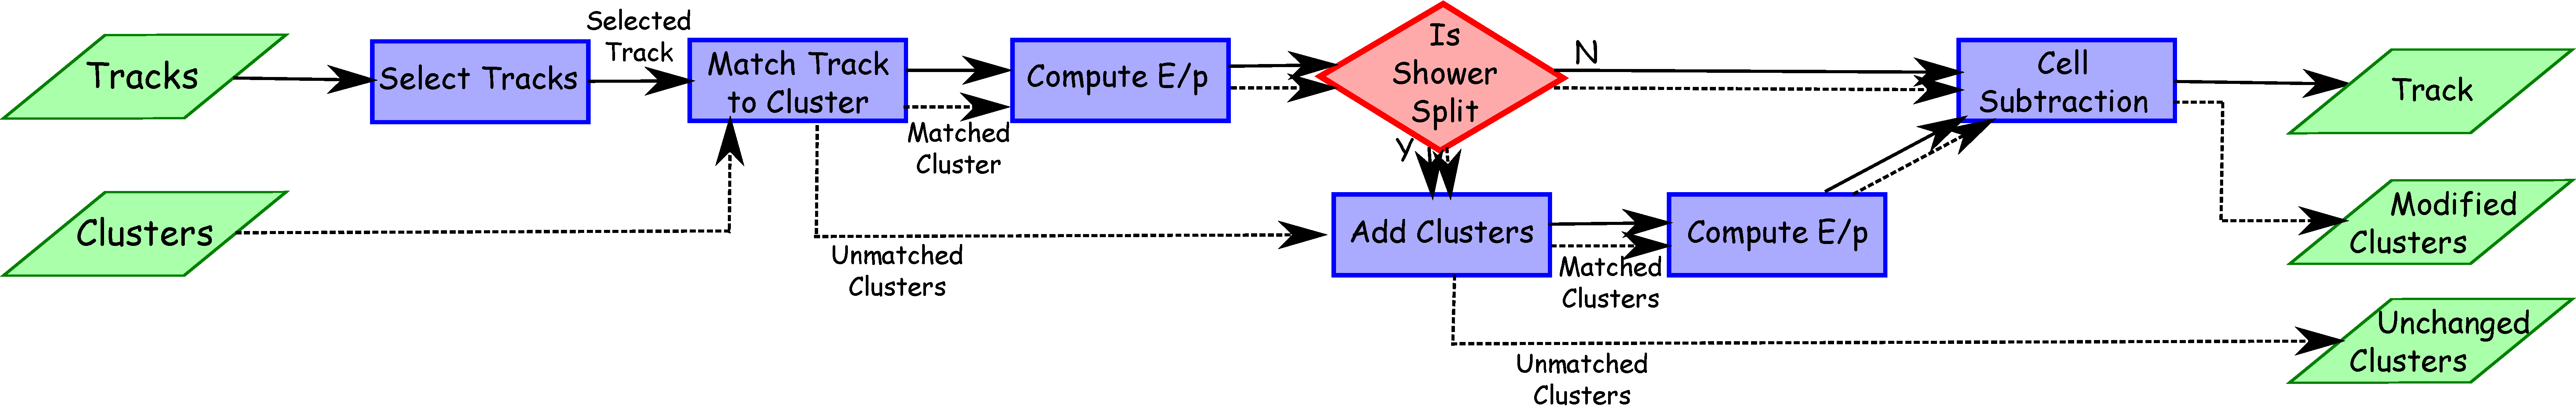
\includegraphics[width=\figwidth]{flowchart.pdf}
  \caption[Flowchart of the steps of the Particle Flow algorithm]{Flowchart of the steps of the Particle Flow algorithm \cite{pflow16}}
  \label{fig:pflowflowchart}
\end{figure}

\subsection{Track selection}

In spite of the clusters the algorithm has some requirements on tracks to be selected to minimize the amount of fake tracks. The requirements are at least 9 hits in the PIXEL and SCT and no missing hits in the PIXEL at all. The tracks have to be in a pseudo-rapidity region of $|\eta|<2.5$ and $\SI{500}{\MeV}<p_T<\SI{40}{\GeV}$.

%check with twiki trackselection



\subsection{Clustering}

The algorithm uses given information from the tracker and the calorimeter as input. The information from the calorimeter is give as topological clusters. The construction of these clusters is briefly described in this chapter to give the reader a basic understanding which input information the algorithm uses.

Each cluster is being constructed around a so called seed cell. A seed cell is a cell for which the deposited energy exceeds the expected noise by four times the standard deviation. If a seed is found all the neighboring cells which exceed the noise by at least two times the standard deviation are added to the cluster. Finally all the cells neighboring these clusters are also added.


\subsection{Matching track to cluster}

The algorithm tries to match every track to one or more calorimeter clusters. First the algorithm tries to match a single best-match topo-cluster to every selected track.
To do so the distances in $\Delta \phi$ and $\Delta \eta$ from the track are extrapolated to the second layer of the EM calorimeter and the topo-clusters. After that the topo-clusters get ranked based on the metric:

\begin{equation}
\Delta R' = \sqrt{\left(\frac{\Delta \phi}{\sigma_{\phi}}\right)^2+\left(\frac{\Delta \eta}{\sigma_{\eta}}\right)^2}
\end{equation}

where $\sigma_{\eta}$ and $\sigma_{\phi}$ refer to the angular topo-cluster width, computed from the standard deviation of the displacemtens of the topo clusters. If the energy in this cluster is greater than or equal to the energy estimated from the track's $p_T$ the algorithm goes to cell subtraction. If the energy in the cluster is smaller than the expected enegery all clusters in a cone of $\Delta R < 0.2$ are matched to the track. In that case R is calculated by the metric:

\begin{equation}
\Delta R = \sqrt{(\Delta \phi)^2 + (\Delta \eta)^2}
\end{equation}

\subsection{Cell Subtraction}

The last step in the Particle Flow algorithm after matching a set of topo-clusters to a track is the cell-wise subtraction of energy deposits to remove remnants and determine which energy depositions belong to the given particle.
If the energy deposited in the set of clusters falls below the expected energy the clusters are simply removed. Otherwise, a cell by cell subtraction is performed.

The first step of the cell subtraction is generating a shower shape from the extrapolated track. Around the extrapolated track rings in $\eta$, $\phi$ space are generated just wide enough to independently contain at least one one cell from the extrapolated position. Furthermore the rings are restricted to one layer and of the same radial size for each layer.
After the generation of rings in each layer the average energy density in each ring is computed and the rings are ranked by energy density in descending order. The layer is not used in any way for this ranking.
The subtraction then starts from the ring with highest energy density and proceeds successively to rings of lower order until the next ring's energy exceeds the remaining expected energy.
If the ring's energy exceeds the energy still to be substracted the energy in each cell is scaled down by the fraction needed to reach the expected energy before the process halts and the remaining cells are removed as remnants.
An example of the process is sketched in figure \ref{fig:sub}. 




\begin{figure}[htbp]
  \centering
  \begin{subfigure}[b]{0.3\figwidth}
    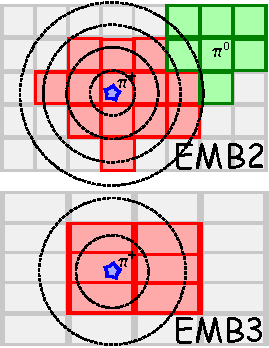
\includegraphics[width=0.25\figwidth]{a}
    \caption{}\label{fig:sub-a}
  \end{subfigure}
  \begin{subfigure}[b]{0.3\figwidth}
    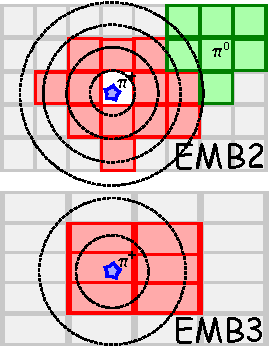
\includegraphics[width=0.25\figwidth]{b}
    \caption{}\label{fig:sub-b}
  \end{subfigure}
  \begin{subfigure}[b]{0.3\figwidth}
    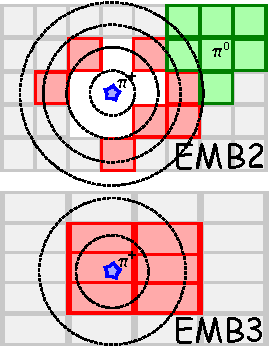
\includegraphics[width=0.25\figwidth]{c}
    \caption{}\label{fig:sub-c}
  \end{subfigure}
  \begin{subfigure}[b]{0.3\figwidth}
    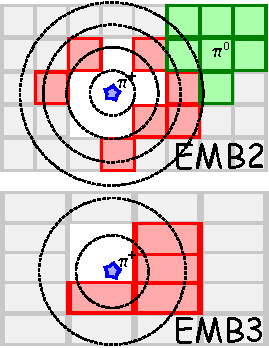
\includegraphics[width=0.25\figwidth]{d}
    \caption{}\label{fig:sub-d}
  \end{subfigure}
    
    
  \begin{subfigure}[b]{0.3\figwidth}
        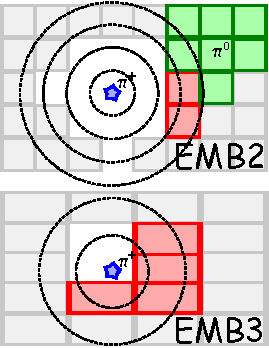
\includegraphics[width=0.25\figwidth]{e}
        \caption{}\label{fig:sub-e}
  \end{subfigure}
  \begin{subfigure}[b]{0.3\figwidth}
        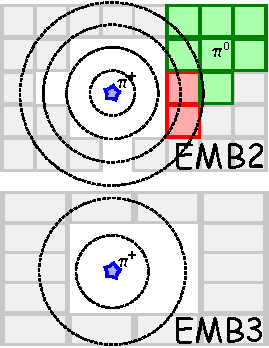
\includegraphics[width=0.25\figwidth]{f}
        \caption{}\label{fig:sub-f}
  \end{subfigure}
  \caption{Example of cell subtraction. In red the depositions originating from the $\pi ^+$ of interest are shown and in green a cluster from a $\pi ^0$ are shown. \cite{pflow16}}
  \label{fig:sub}
\end{figure}

%add a reference here. wildcard there

\subsection{Eflow Rec performance studies}

The Particle Flow manuscript shows the impact of the new algorithm on the angular resolution and on the rejection of pileup jets. This section briefly summarizes the important results of this study. Figure \ref{fig:etarun1} and \ref{fig:phirun1} show the improvements in angular resolution while figure \ref{fig:pileuprun1} displays the increased rejection of fake jets for the new algorithm. LC+JES jets are the jets using the old algorithm and JVF in figure \ref{fig:pileuprun1} refers to the Jet Vertex Fraction representing the amount of energy in the jet originating from the original vertex.

The plots clearly demonstrate that Particle Flow does improve the angular resolution in low $p_T$ regions while having no drawback for higher $p_T$ regions. The pileup contribution is also mediated massively even in comparison to the usage of a cut on the JVT. The region of effect is restricted to $|\eta|<\num{2.5}$ because only this region of pseudorapidity is covered by the Inner Detector. Only the momentum resolution shown in figure \ref{fig:ptrun1} worsens using the old reconstruction for high $p_T$ regions.
%JVT sentence
\begin{figure}[h]
  \centering
  \begin{subfigure}[b]{0.5\figwidth}
  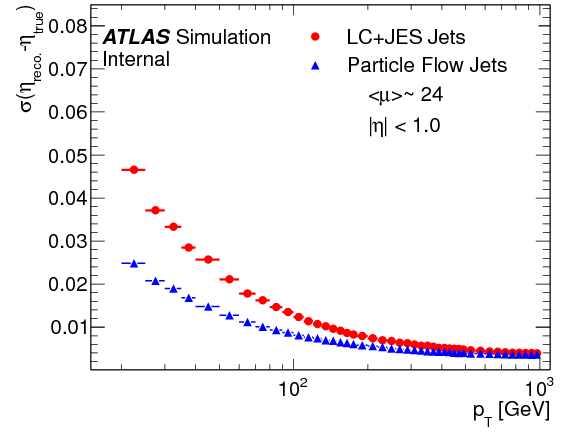
\includegraphics[width=0.5\figwidth]{etarun1.png}
  \caption[Improvements in $\eta$ resolution for Particle Flow Jets]{Improvements in $\eta$ resolution for Particle Flow Jets \cite{pflow16}}
  \label{fig:etarun1}
  \end{subfigure}
  \begin{subfigure}[b]{0.5\figwidth}
  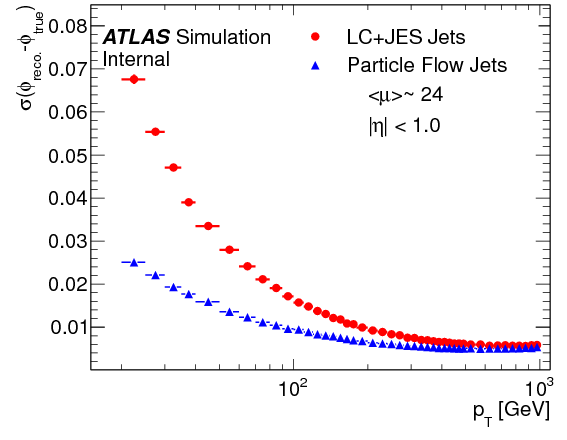
\includegraphics[width=0.5\figwidth]{phirun1.png}
  \caption[Improvements in $\phi$ resolution for Particle Flow Jets]{Improvements in $\phi$ resolution for Particle Flow Jets \cite{pflow16}}
  \label{fig:phirun1}
  \end{subfigure}
\end{figure}

\begin{figure}[h]
  \centering
  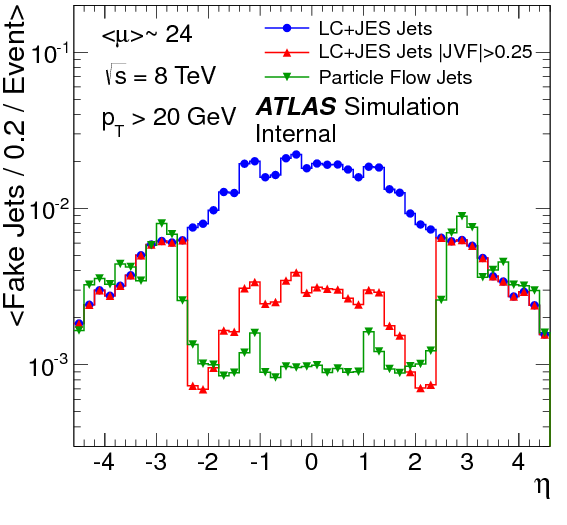
\includegraphics[width=0.8\figwidth]{pileuprun1.png}
  \caption[Pileup comparison of EM-Topo Jets and Particle Flow jets]{Pileup comparison of EM-Topo Jets and Particle Flow jets \cite{pflow16}}
  \label{fig:pileuprun1}
\end{figure}

\begin{figure}
\centering
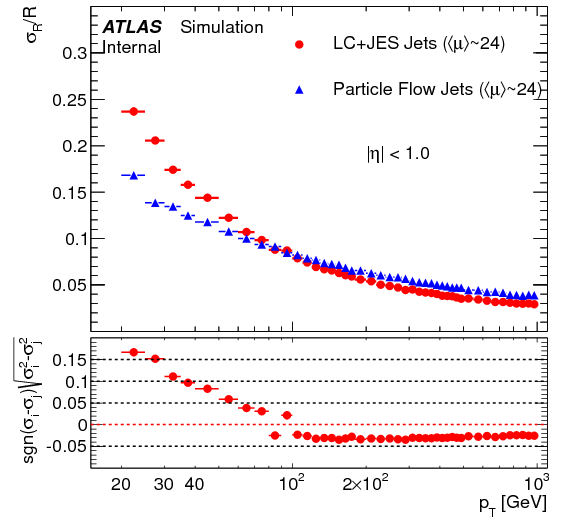
\includegraphics[width=0.8\figwidth]{ptrun1.png}
\caption[Momentum resolution of Particle Flow]{Momentum resolution of Particle Flow jets \cite{pflow16}}
\label{fig:ptrun1}
\end{figure}



\subsection{Recent updates in eflowrec}

The description of the Particle Flow algorithm given in this thesis is based on the analysis of Run 1 data and some recent changes to the algorithm are described in this section.


%Here I want to explain what tools are used for PFlow already and what tools are %missing.
%Then I should focus on which tools have been implicitly upgraded
%Problematic right now are the cleaning the trigger matching the pileup reweithing %and the complete JES

\chapter{Analysis framework}

In order to construct a framework for general Particle Flow analysis and data Monte Carlo comparison a large amount of ingredients is needed to be included and checked to be correctly working. In this chapter I will go over the important tools included in my framework. The impact of every given tool will be demonstrated and possible problems in current implementation are also included to summarize the status of the framework.
The description starts with the event selection. The second section describes the trigger system and its corresponding tools and finally the calibrations for specific objects are introduced.

In addition to that a further section describes the changes that have to be made to find a good matching of data and Monte Carlo.

%should the event selection be here ?



\section{Event selection}

\subsection{The Good Run List}

Before any analysis or calibration takes place the good run list has to be checked. The Good Run List is only needed for actual detector data.

For data to be suitable fo analysis one has to make sure that it fits certain requirements of which some depend on the detectors working state. The Good Run List allows to exclude data-taking periods in which the detector showed a poor working state. Reasons for this may be maintenance on sub detectors, magnets off or ramping or an unstable beam of the LHC.
The Good Run List includes all the good data taking periods and the tool excludes all data from bad periods.
For the data analysis in this thesis the recommended GRL for 2016 data wildcard was used.


\subsection{Event cleaning}

Additionally to the cuts provided due to the GRl some further events have to be excluded. Noise bursts and corrupted data in general have to be removed in the LAr, the SCT and the Tile. Furthermore due to production errors some events might be duplicant and have to be removed. 

%what does this mean


\section{Trigger Tools}

A further important collection of tools has to make sure that the trigger is fired, correctly used and also that the particle that triggered is actually one of those used in later analysis.

\subsection{Trigger system}


A trigger basically is a first selection for an event meaning that an event is required to surpass certain demands to be used in analysis. These demands are embodied by so called trigger chains that can be used as input for a trigger tool in analysis which on that base can select or refuse events. For the analysis in this thesis the recommended single lepton triggers for 2016 data were used. The chains were HLT_mu26_ivarmedim, HLT_mu50.



\subsection{Trigger matching}

Usually the trigger is checked before the event is further cleaned and calibrated. Therefore it can happen that the particles that passed the trigger later get removed in the analysis. The trigger matching makes sure that the particles that passed the triggers are still left in the final analysis and if not the event can still be removed.

\section{Monte Carlo Re-weighting and scale factors}

The Monte Carlo is produced before data is taken therefore the shape of Monte Carlo may vary from the shape of the actual taken data for several reasons. For example the pileup in MC may not match the data as well as the resolution. To compensate these differences a sum of weights is applied to Monte Carlo as well as to data.

\subsection{Data Re-weighting}

\subsection{Monte Carlo re-weighting}

\subsection{Lepton scale factors}

To the electrons and muons additional scale factors (SF) are applied to accomodate the differences between data and simulation of these particles.

\section{Object calibration and selection}

The last step in the framework is the selection and calibration of the objects in a given event. This section summarizes the tools needed not only for jets but also for muons electrons, which are the objects used in the Monta Carlo data comparison in the following chapter.

\subsection{Jet cleaning}

Before the jets in an event are scaled or further calibrated the jet calibration takes place. The jet cleaning allows to apply certain requirements on jets in an event and therefore to remove jets or even complete events that might be bad data. The Jet Cleaning is used on both data and Monte Carlo to make sure that Monte Carlo events that would be removed in data also are not included in the simulation.
Bad jets are excluded on the base of their wildcard.
For this framework a wildcard selection has been chosen and if one bad jet is found the whole event is removed.

\subsection{Jet Calibration and Smearing}

After making sure a jet is "good" and therefore has passed the cleaning it must still be be calibrated and in case of MC smeared to data. The Calibration scales the energy of jets for a certain reconstruction algorithm. The Smearing smears the MC resolution to be matching the actual data resolution.


\begin{figure}
\centering
\begin{subfigure}[b]{0.5\figwidth}
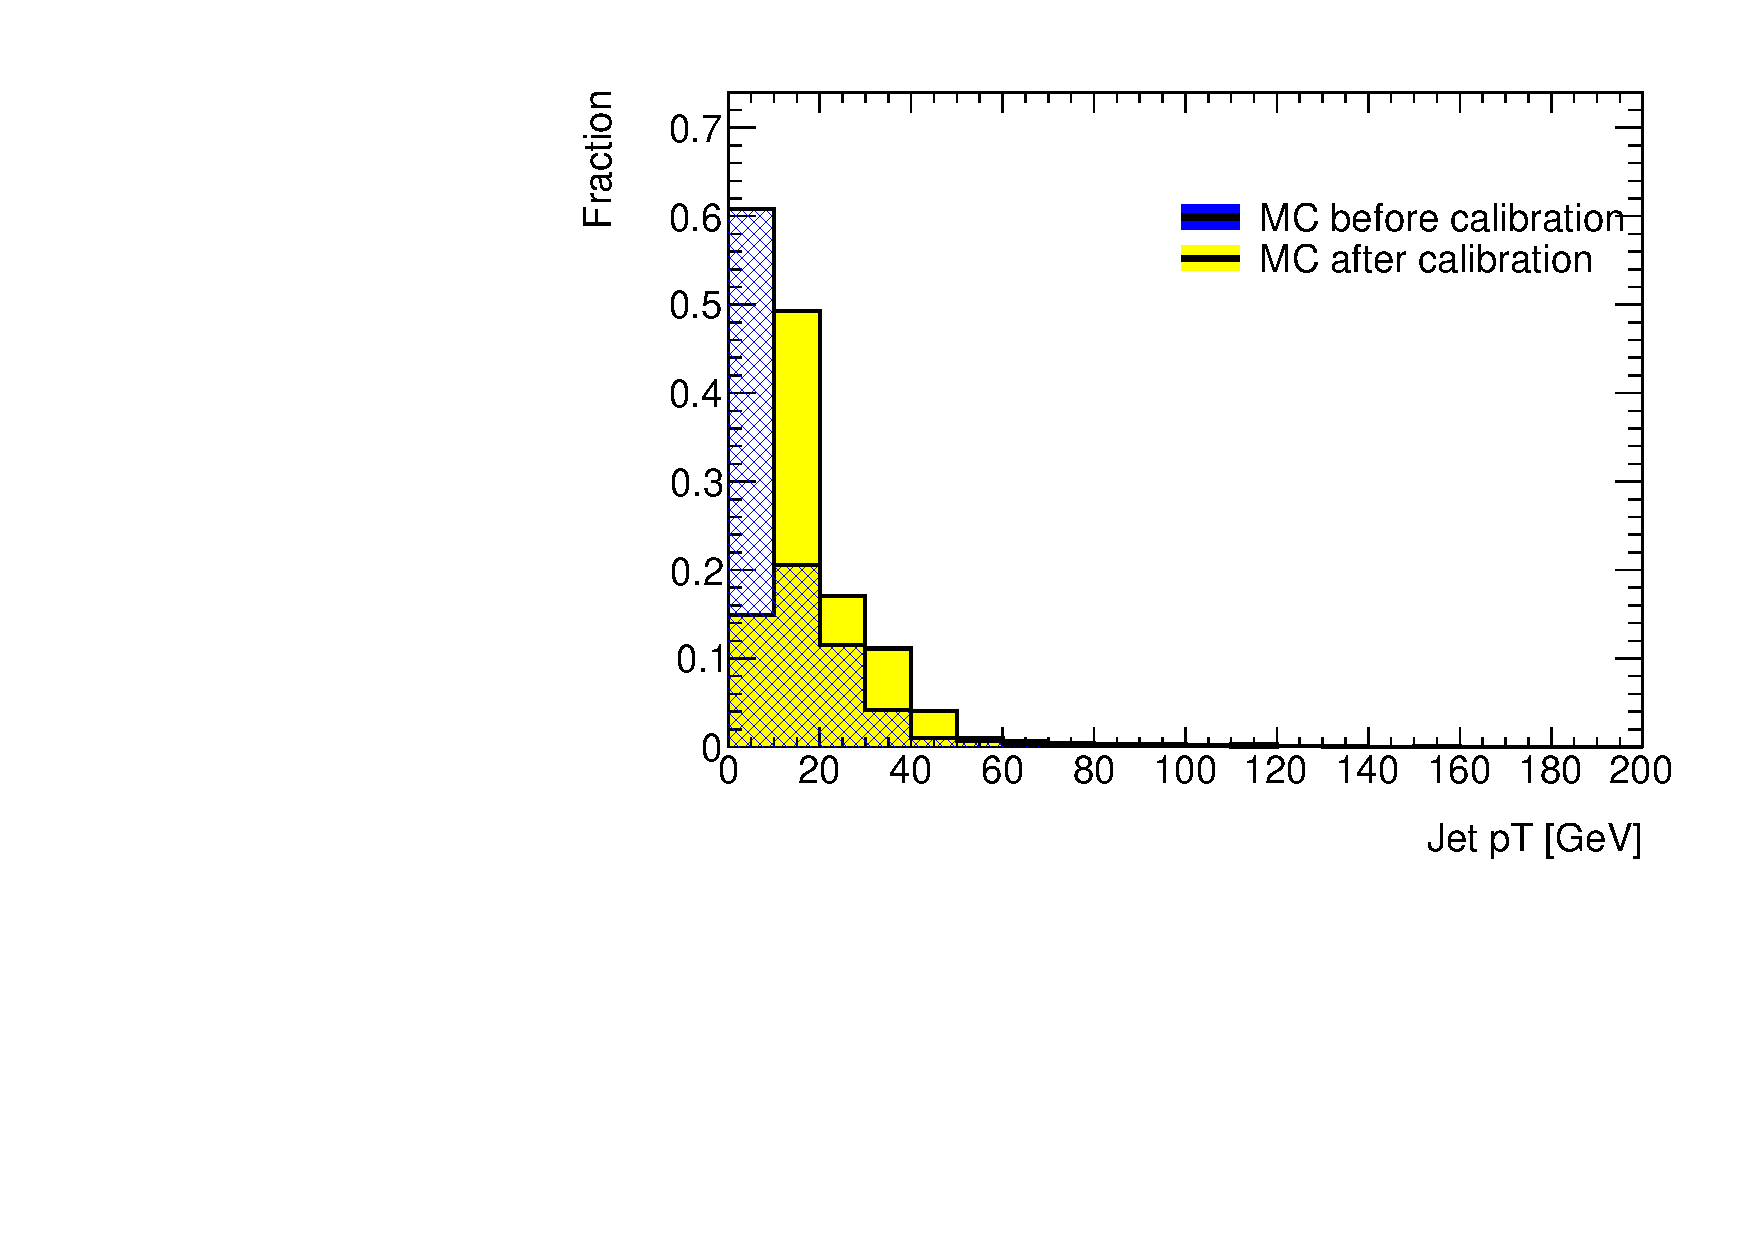
\includegraphics[width=0.53\figwidth]{testscalingpt}
\caption[Influence of the JES on the transversal momentum]{The influence of the calibration in momentum is shown}
\label{fig:testscalingpt}
\end{subfigure}
\quad
\begin{subfigure}[b]{0.5\figwidth}
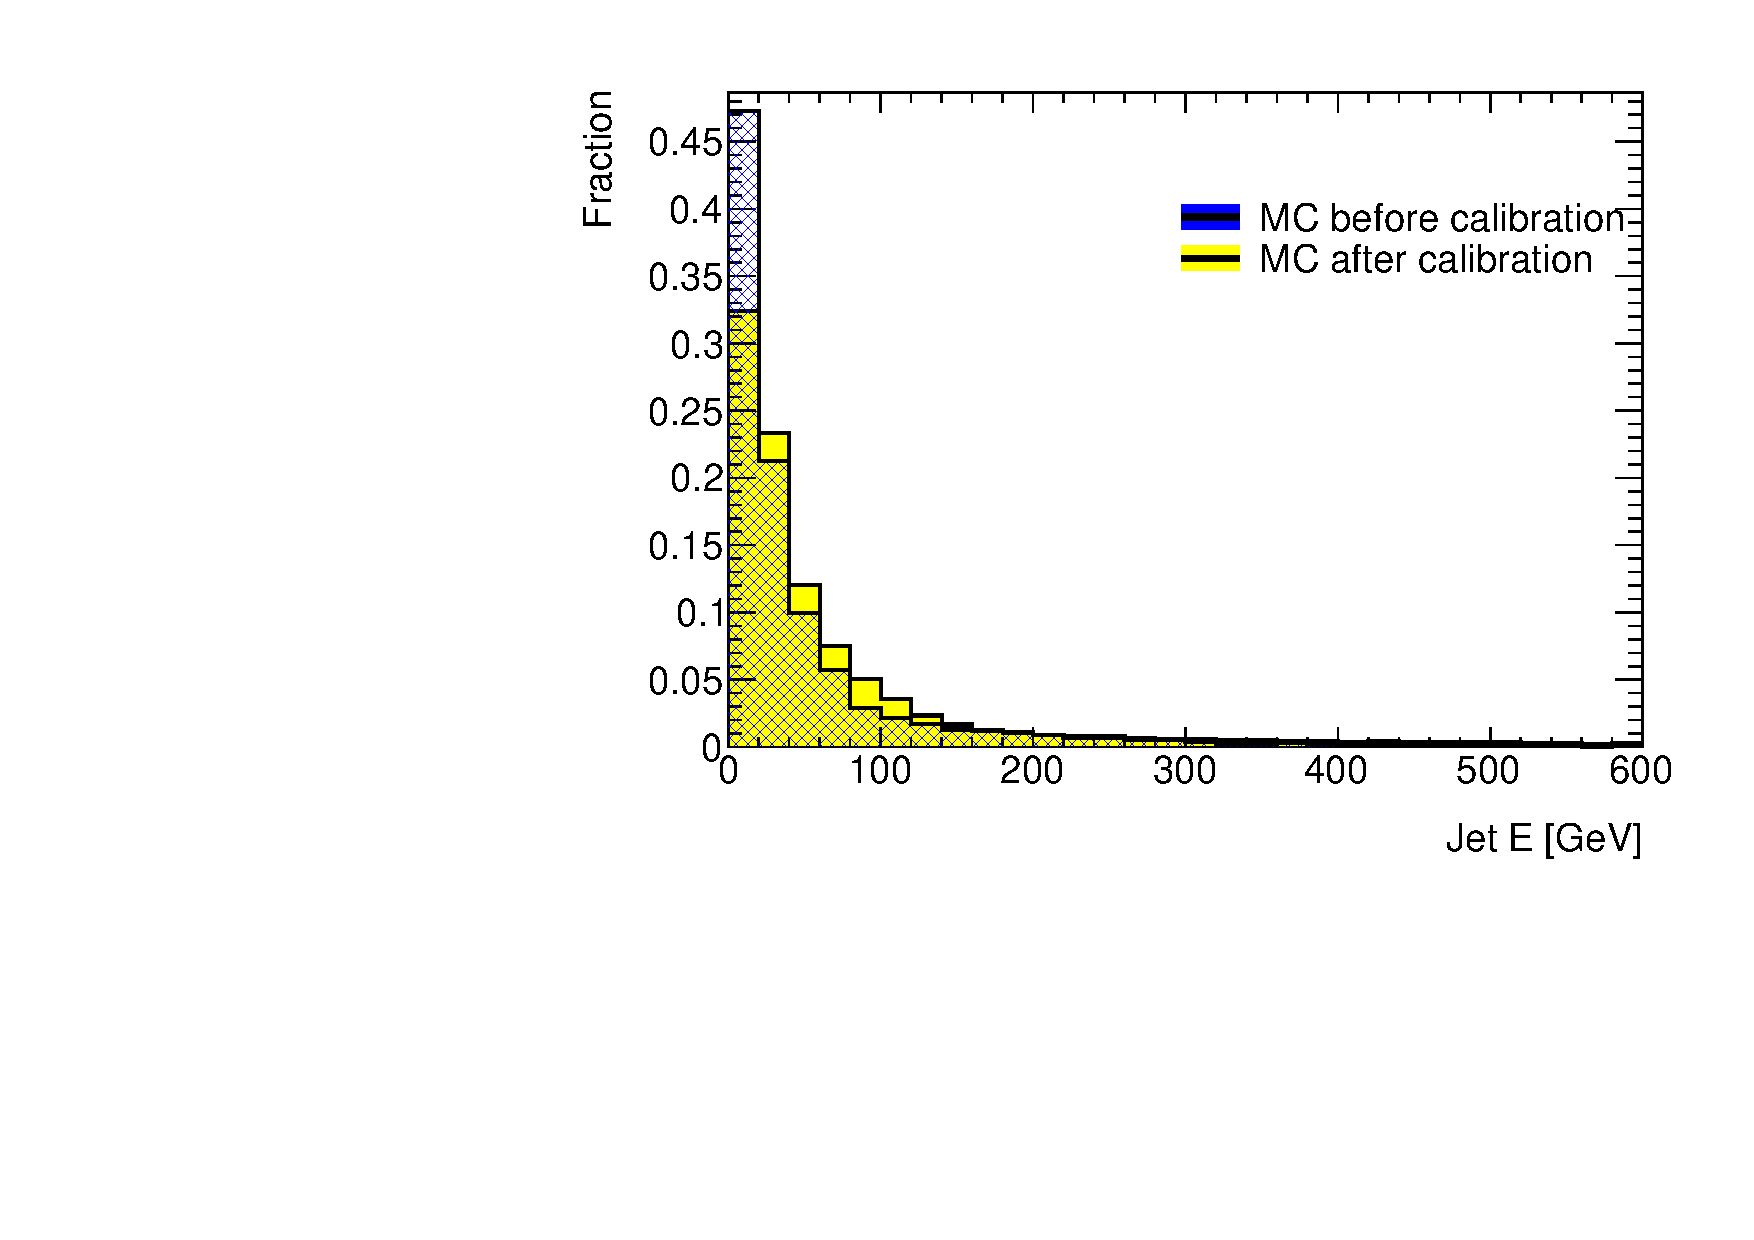
\includegraphics[width=0.53\figwidth]{testscalinge}
\caption[Influence of the JES on the energy]{The influence of the calibration in energy is shown}
\label{fig:testscalinge}
\end{subfigure}
\end{figure}


\begin{figure}
\centering
\begin{subfigure}[b]{0.5\figwidth}
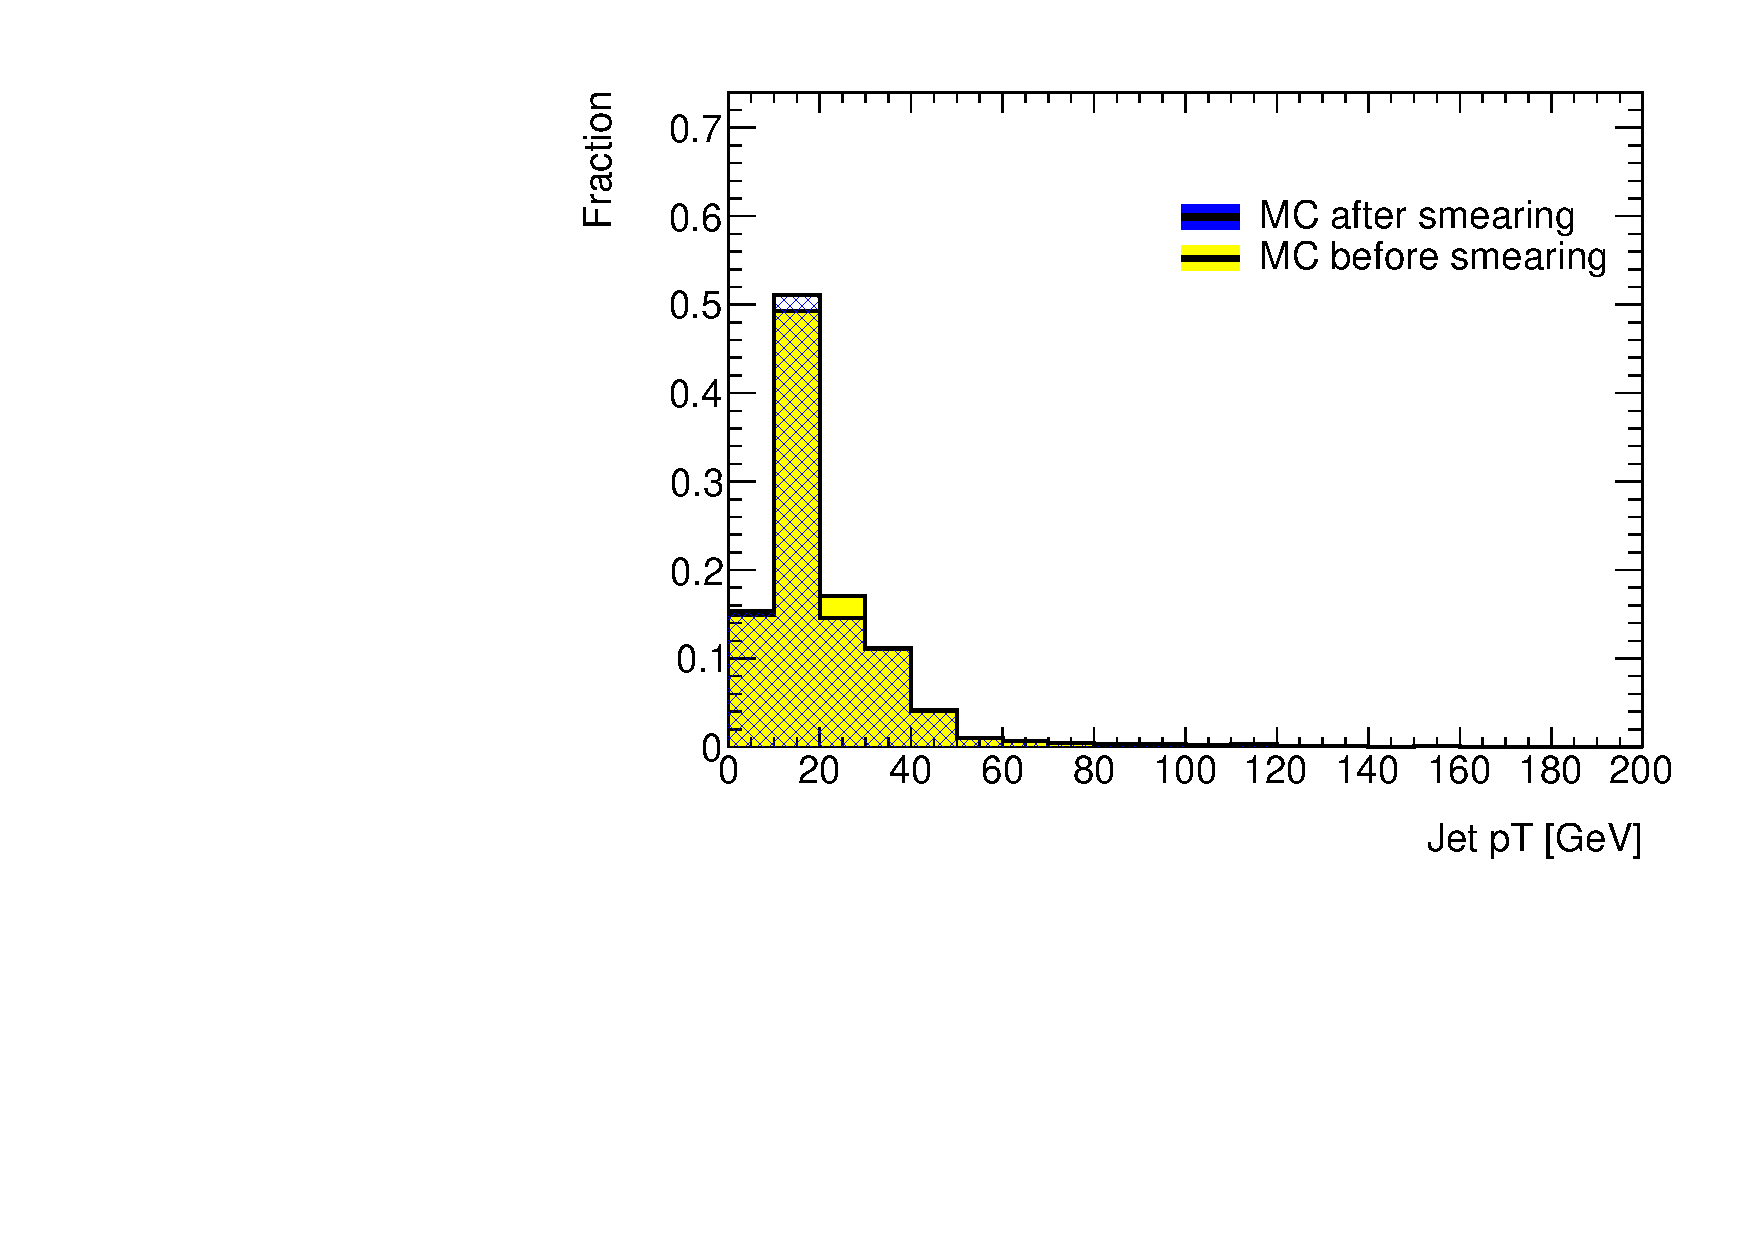
\includegraphics[width=0.53\figwidth]{testsmearingpt}
\caption[Influence of the Smearing on the transversal momentum]{The influence of the Smearing in momentum is shown}
\label{fig:testsmearingpt}
\end{subfigure}
\quad
\begin{subfigure}[b]{0.5\figwidth}
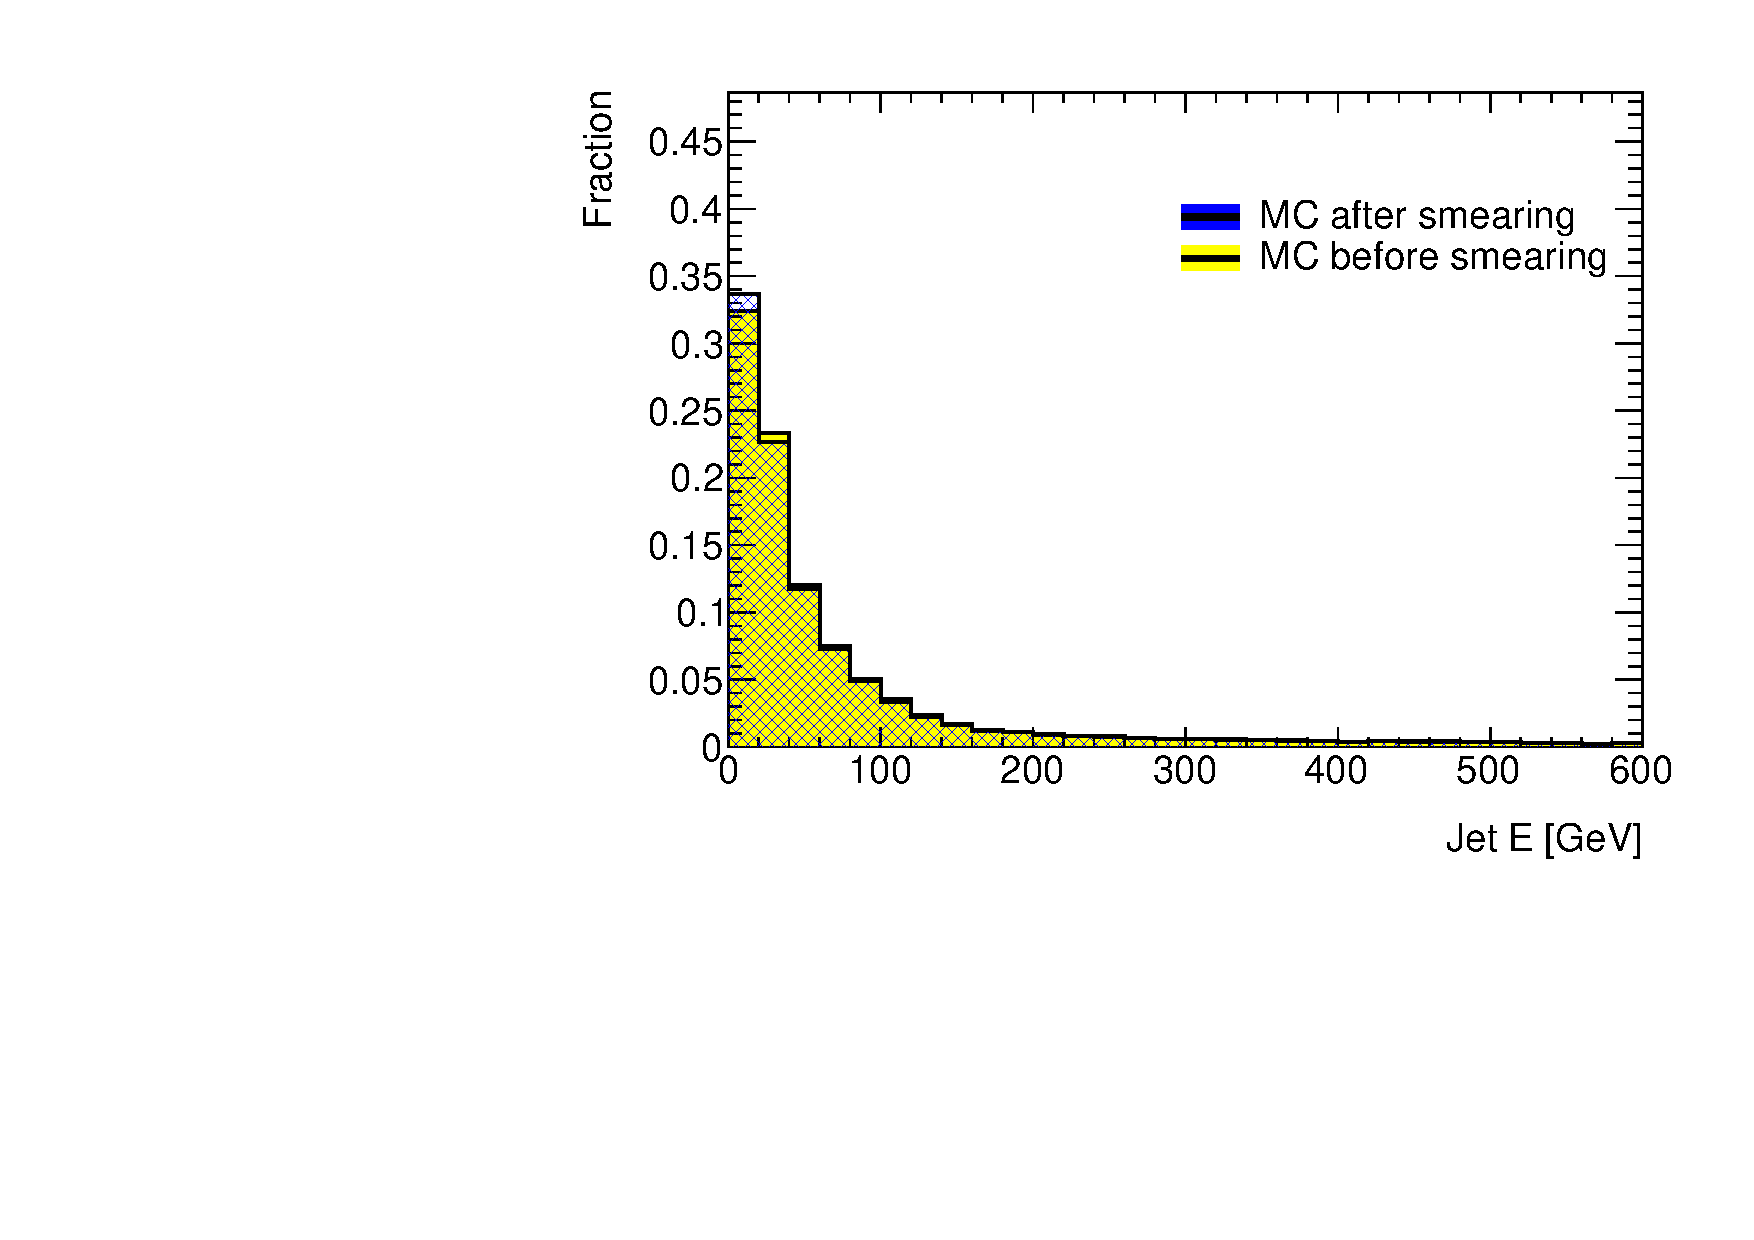
\includegraphics[width=0.53\figwidth]{testsmearinge}
\caption[Influence of the Smearing on the energy]{The influence of the Smearing in energy is shown}
\label{fig:testsmearinge}
\end{subfigure}
\end{figure}


\subsection{The jet vertex tagger}

Due to the high luminosity at the LHC in time and in space pileup is a big problem in ATLAS analysis. Therefor the rejection of pileup is an important part of analysis. One possible way to minimize pileup is to calculate the jet-vertex fraction of each jet which is the fraction of momentum in the jet originating from the primary vertex. If one sets a minimum on this fraction pileup can be suppressed because jets that do not pass the criteria on their JVF are highly likely to be originating from pileup vertices. The Jet Vertex Tagger relates each jet to a vertex.


\subsection{Muon Calibration and Selection}

Analog to jets the muons in an event also have to go through several cuts and have to be calibrated properly. This section introduces all the important tools for muon calibration and gives a brief summary of the effects of the cuts and calibrations.
The first and foremost task of the mun tools is to determine whether a muon originated from the original vertex or has its origin in background noise( cosmic muons) or in some kind of secondary interaction. Muons are reconstructed using both the muon spectrometers and the inner detector. The information from both detector systems is combined to a single track. Then the muons are requested to have $p_T > \SI{25}{\GeV}$ and a pseudorapidity of $|\eta| < \num{2.5}$. To reject the cosmic muon background further the muons are not allowed to have a longid´tudinal impact paramter to the primary vertex that is higher than \SI{3}{\mm}. The last requirement is added due to muons originating from heavy flavour quark decays. 

To remove these last unwanted muons an isolation criteria is implemented, namely the isolation tool. The tool makes sure that the sum of transversal momentum of the tracks around the muon candidate divided by the muons momentum is smaller than \num{0.05}. 

\begin{equation}
\frac{\sum_{\Delta R}pT_{track}}{pT_{\mu}} < 0.05
\end{equation}

This way in $Z \rightarrow \mu^+ \mu^-$ events an efficiency of \num{97} \% in muon detection was achieved.

The second part of the muon tools makes sure that the muon properties are correctly calibrated and smeared to make Monte Carlo and data match properly and to eliminate known weaknesses in the detector structure. Figure \ref{fig:testmuonpt} shows the muons transversal momentum before and after calibration in Monte Carlo. The changes are very minor.

\begin{figure}[h]
\centering
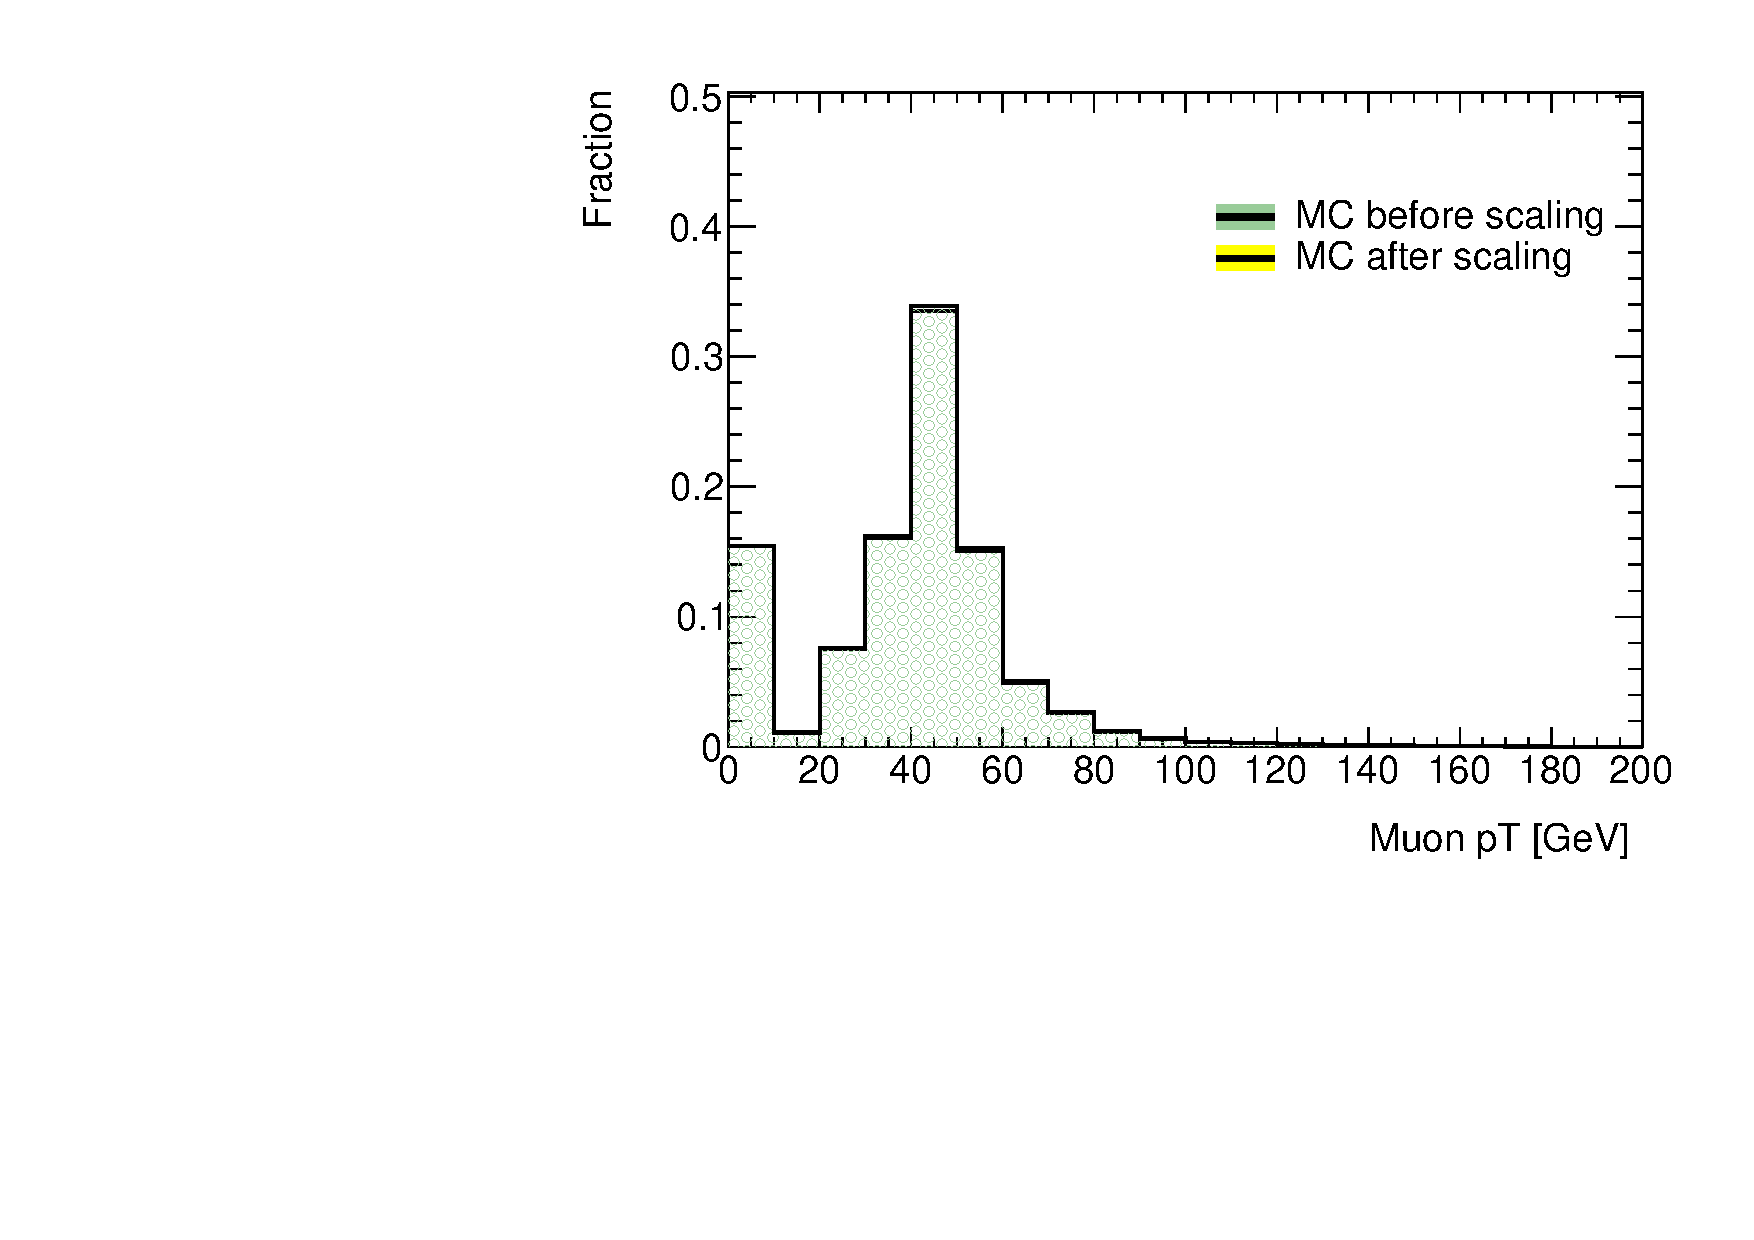
\includegraphics[scale=0.7]{testmuonpt}
\caption{Calibration and smearing of the muon momentum. The changes are very minimal.}
\label{fig:testmuonpt}
\end{figure}

\subsection{Electron Calibration and Selection}

The electron tools are the more or the less parallel to the muon tools. There is a first group of tools and criteria to determine which electrons actually originate from the primary vertex and distinguishes those electrons from background and pileup. The second group of tools calibrates the wanted electrons properties.

Electrons are detected by leaing a track in the inner detctor and depositing lose to all of their energy in the electromagnetic calorimeter. The reconstruction algorithm expects a calorimeter cluster with a deposited energy $E_T$ exceeding \SI{2.5}{\GeV}. This cluster has then to have a matching track from the primary hard scatter vertex. The $\eta$ requirements are $|\eta|_{cluster} < 2.47$ with an exclusion of $\num{1.37} < |\eta| < \num{1.52}$ (calorimter barrel-endcap transition region).

Electrons are same as muons required to be isolated. The Isolation is based on a $\Delta R < \num{0.2}$ cone in the deposited energy and a $\Delta R < \num{0.3}$ cone around the track.

The elctron calibration and smearing is exemplary diplayed in figure \ref{fig:testelectronpt}. The impact of the scaling is significantly higher than for muons.

\begin{figure}
\centering
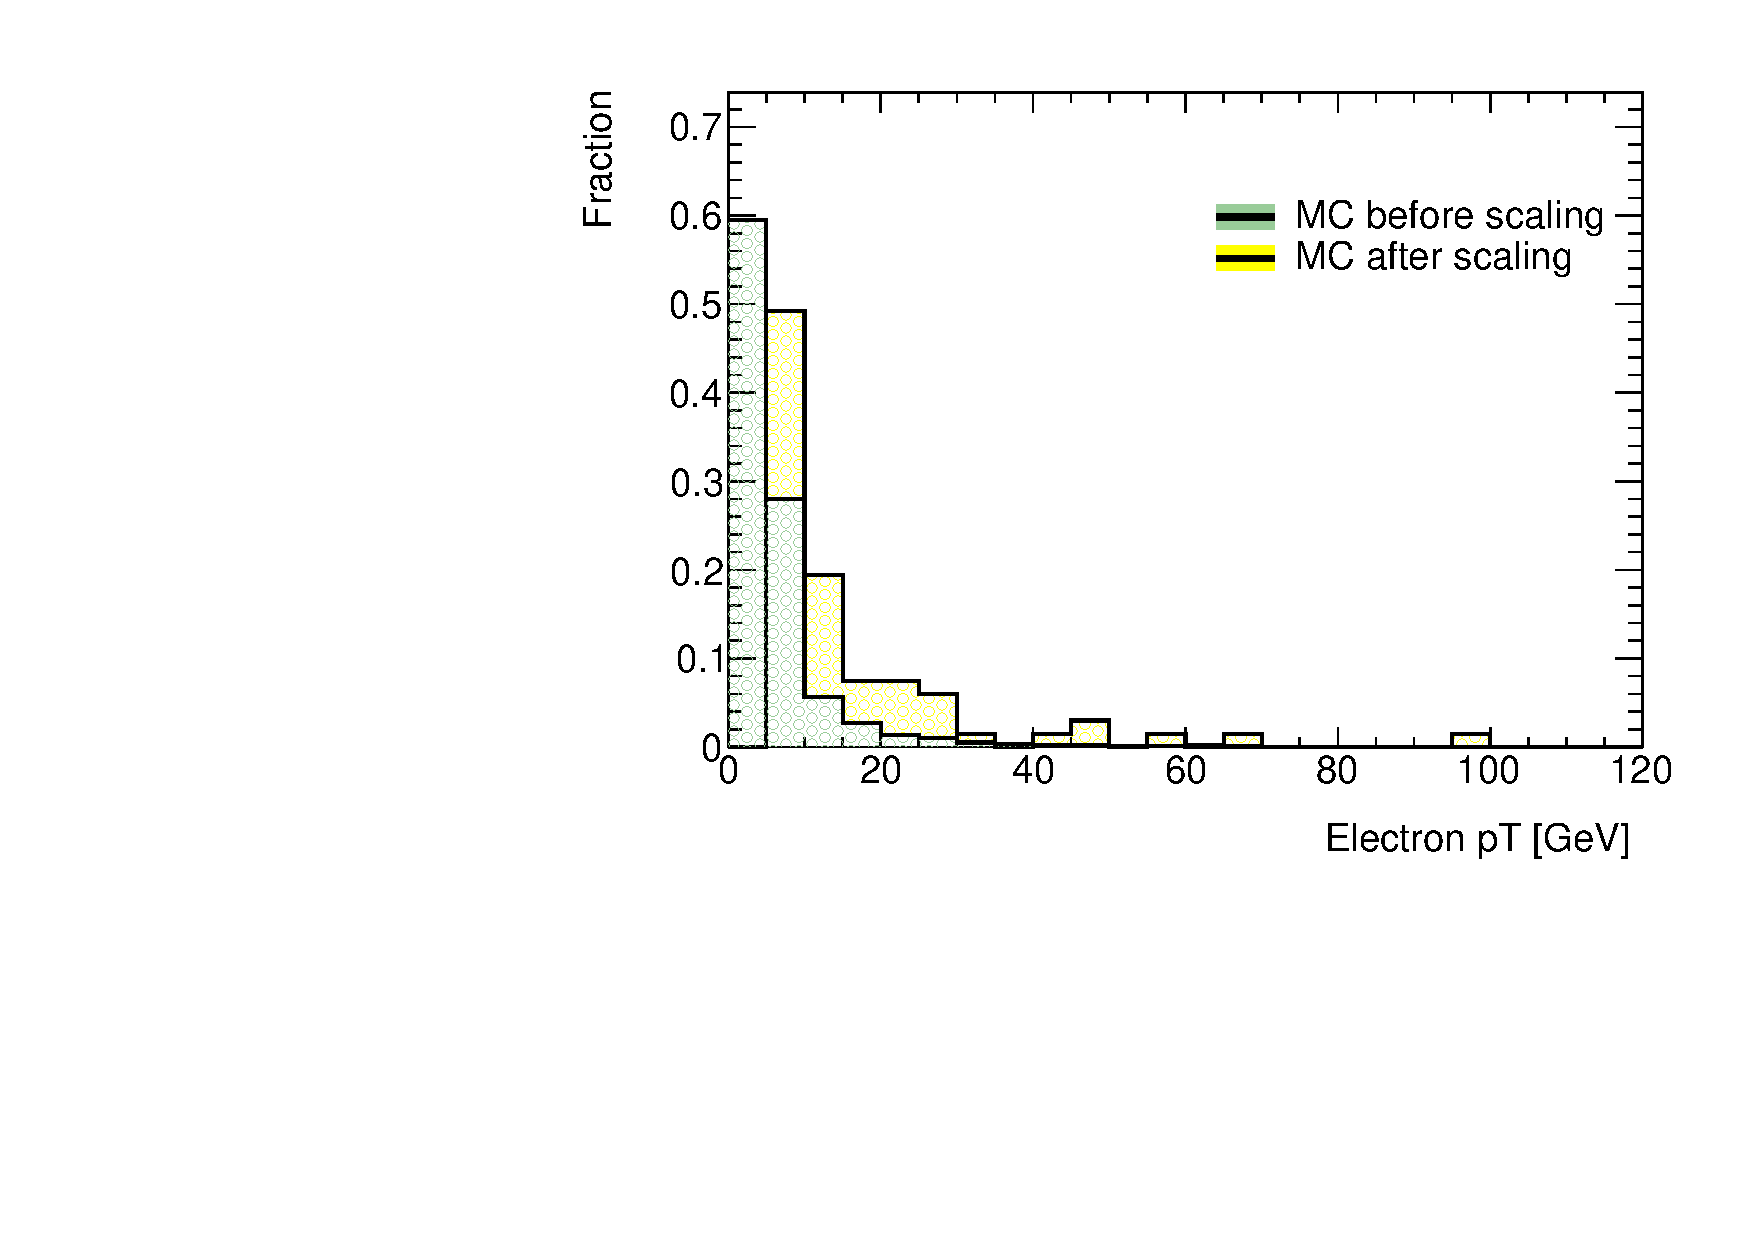
\includegraphics[scale=0.7]{testelectronpt}
\caption{Calibration and smearing of the electron momentum.}
\label{fig:testelectronpt}
\end{figure}

\chapter{Performance of the Particle Flow algorithm in data/MC comparison}

To study the performance of the Particle Flow algorithm in Run 2 data/Monte Carlo comparison a  $Z \rightarrow \mu \mu$ decay has been chosen. The used dataset was wildcard and wildcard was used for the Monte Carlo. The chapter explains the choice of decay and gives a overview over the event selection before showing a summary of performance plots. 

\section{The $Z \rightarrow \mu \mu$ decay}
\begin{figure}[h]\centering
\begin{fmffile}{ztomumu}
\begin{fmfgraph*}(50,30) \fmfpen{thin}
  \fmfleft{i1} \fmfright{o1,o2}
  \fmf{wiggly, label=$Z$}{i1,v1}
  \fmf{fermion, label=$\mu$}{v1,o2}
  \fmf{fermion, label=$\overline{\mu}$}{v1,o1}
  \end{fmfgraph*}
\end{fmffile}
\caption{Decay of a Z-Boson to two muons}
\label{decay}
\end{figure}


For this thesis $Z\rightarrow \mu \mu$ events were used. The deay channel of a $Z$ boson into a muon and a antimuon has a crossection of \num{3.366 +- 0.007} \cite{pdg}. The event was chosen for this analysis because the Z boson is very easy to trigger on and it allows a very clear event selection. Furthermore the event has exactly one recoiling jet that analysis can be performed on. 

\section{Event selection}
The criteria for the event selection were no good electrons and exactly two good muons, with opposite charge where good means that the particle passed all selection filters itself. The muons are required to have a transversal momentum greater than \SI{25}{\GeV}. Furthermore the muons are restricted to a central $\eta$ region being $|\eta|<2.4$.

Furthermore a jet is required to have a transversal momentum greater than \SI{20}{\GeV} and is required to be recoiling to the reconstructed Z giving the selection criteria $|\phi_{jet}-\phi_Z|<(\pi - \num0.4)$.
The region of pseudorapidity is limited to  $|\eta|<2.5$ to ake into account the the inner tracking detector covers only this region.

Figure one shows the number of events selected. 

\section{Kinematic variables of muons and jets}

After selecting proper $Z \rightarrow \mu \mu$ events the agreement between data and MC has been studied for the selected objects. This section summarizes the kinematic variables of the muons and the chosen recoiling jet.

Figure \ref{fig:muons} shows the kinematic variables of the muons. For $pT<\SI{100}{\GeV}$ and $e<\SI{300}{\GeV}$ the agreement between data and Monte Carlo for momentum and energy is very good. In greater momentum regions the agreement worsens significantly. This might have its reason in insufficient statistics. For $\eta$ and $\phi$ the agreement is quite good.

The recoiling jet properties are shown in figure \ref{fig:reoilingjet}. The agreement for $pT$ and energy are rather bad for the jets especially in high energy regions but even in low $pT$ and energy regions the agreement is far worse than expected.
The angular agreement looks better except for $|\eta|>2.5$ which is outside the tracker region and could be excluded for Particle Flow performance analysis.



\begin{figure}[h]
\centering
\begin{subfigure}[b]{0.5\figwidth}
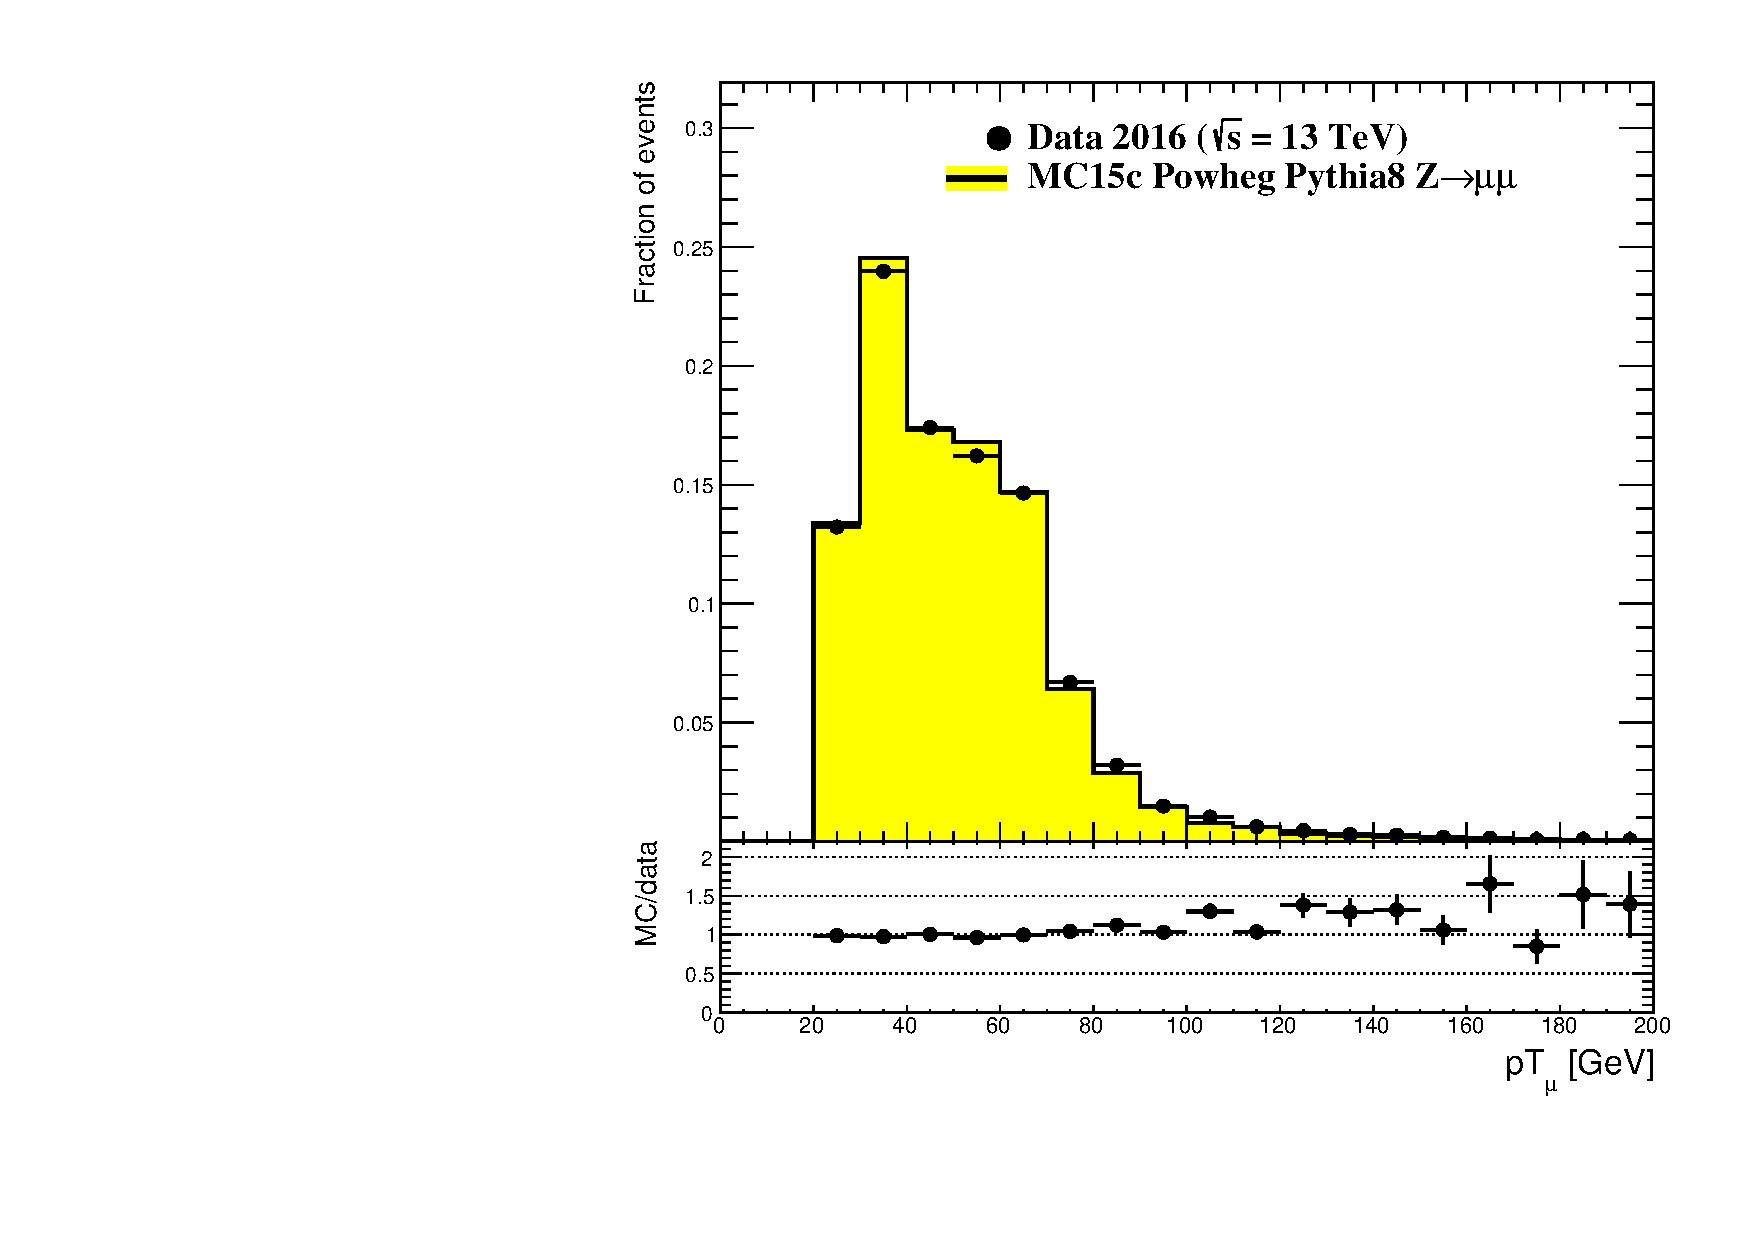
\includegraphics[width=0.53\figwidth]{muon_ptratio}
\caption[Transversal momentum of the muons]{$pT_{\mu}$}
\label{fig:muonpt}
\end{subfigure}
\quad
\begin{subfigure}[b]{0.5\figwidth}
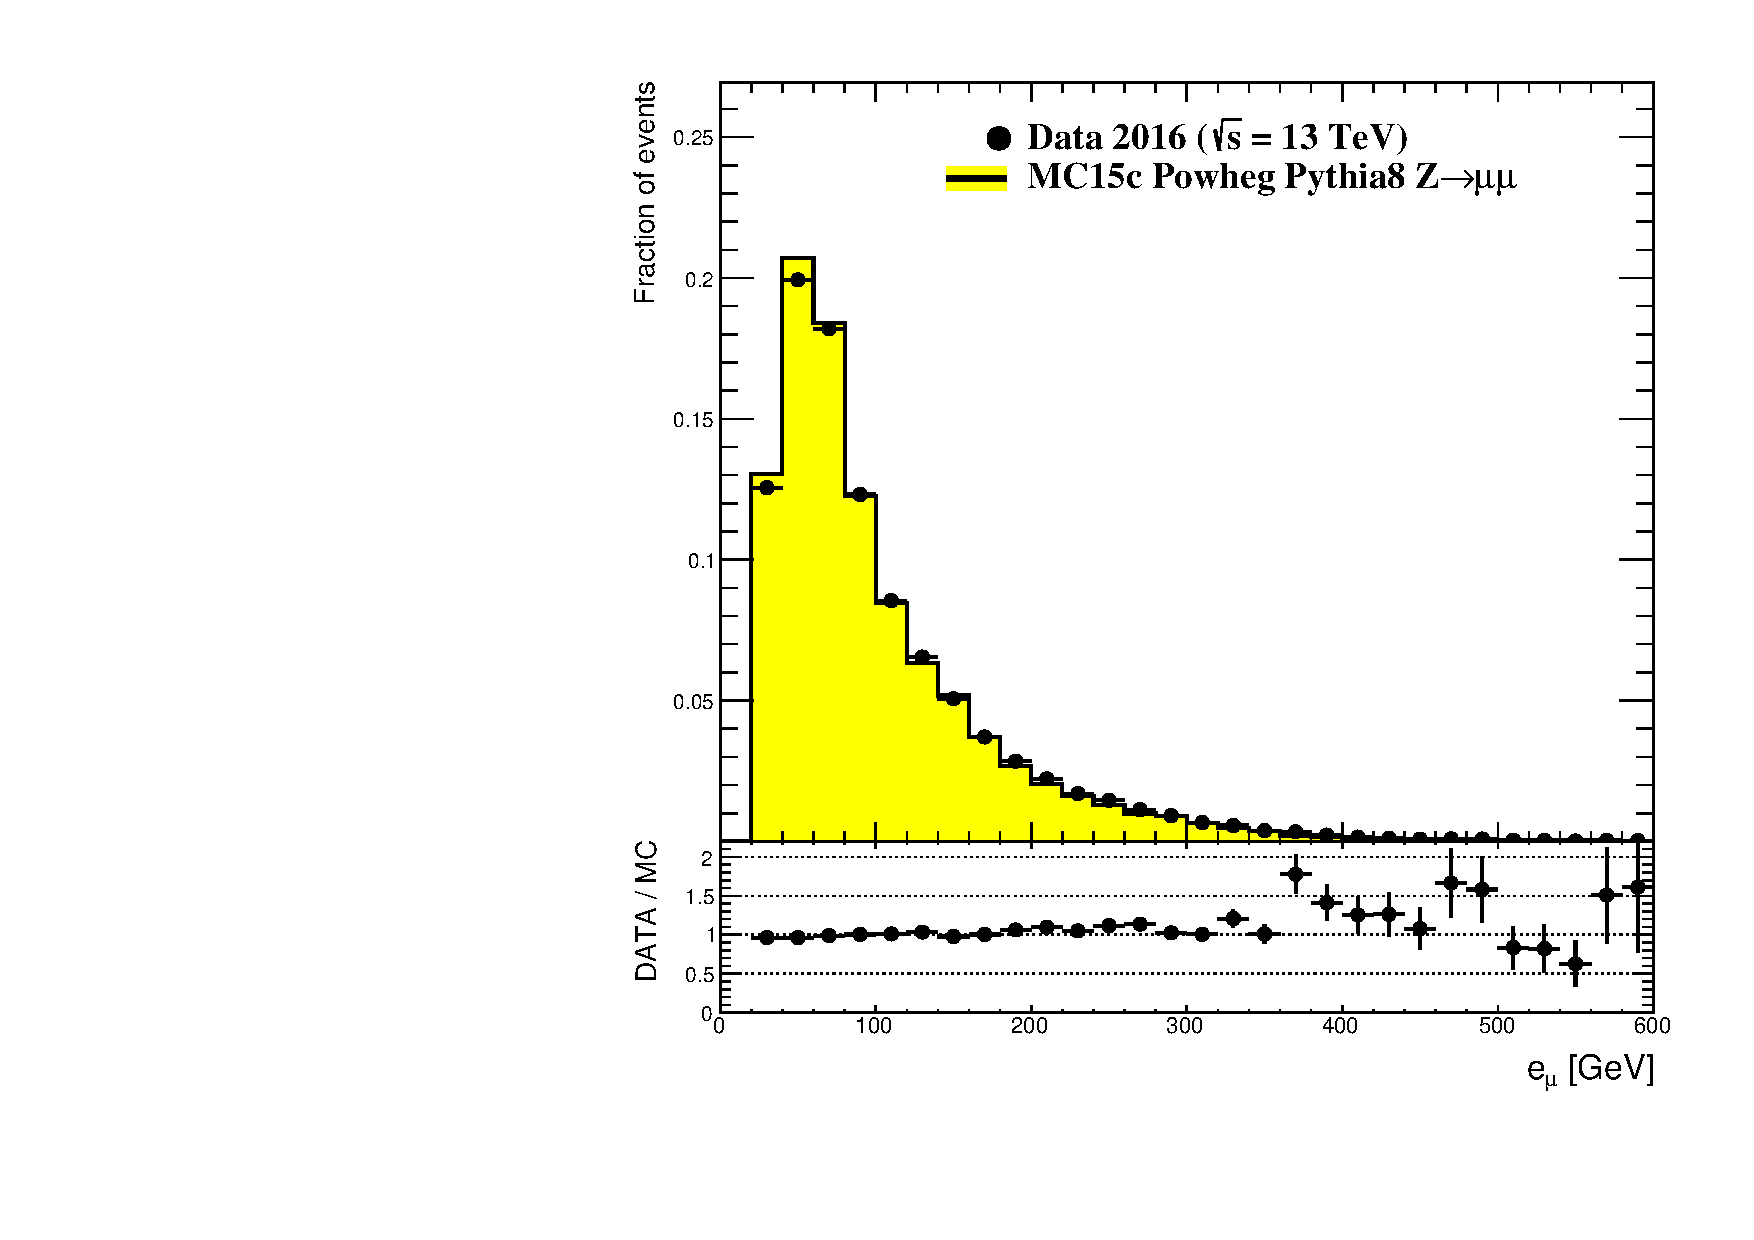
\includegraphics[width=0.53\figwidth]{muon_eratio}
\caption[Energy of the muons]{$e_{\mu}$}
\label{fig:muone}
\end{subfigure}
\end{figure}


\begin{figure}[h]
\centering
\begin{subfigure}[b]{0.5\figwidth}
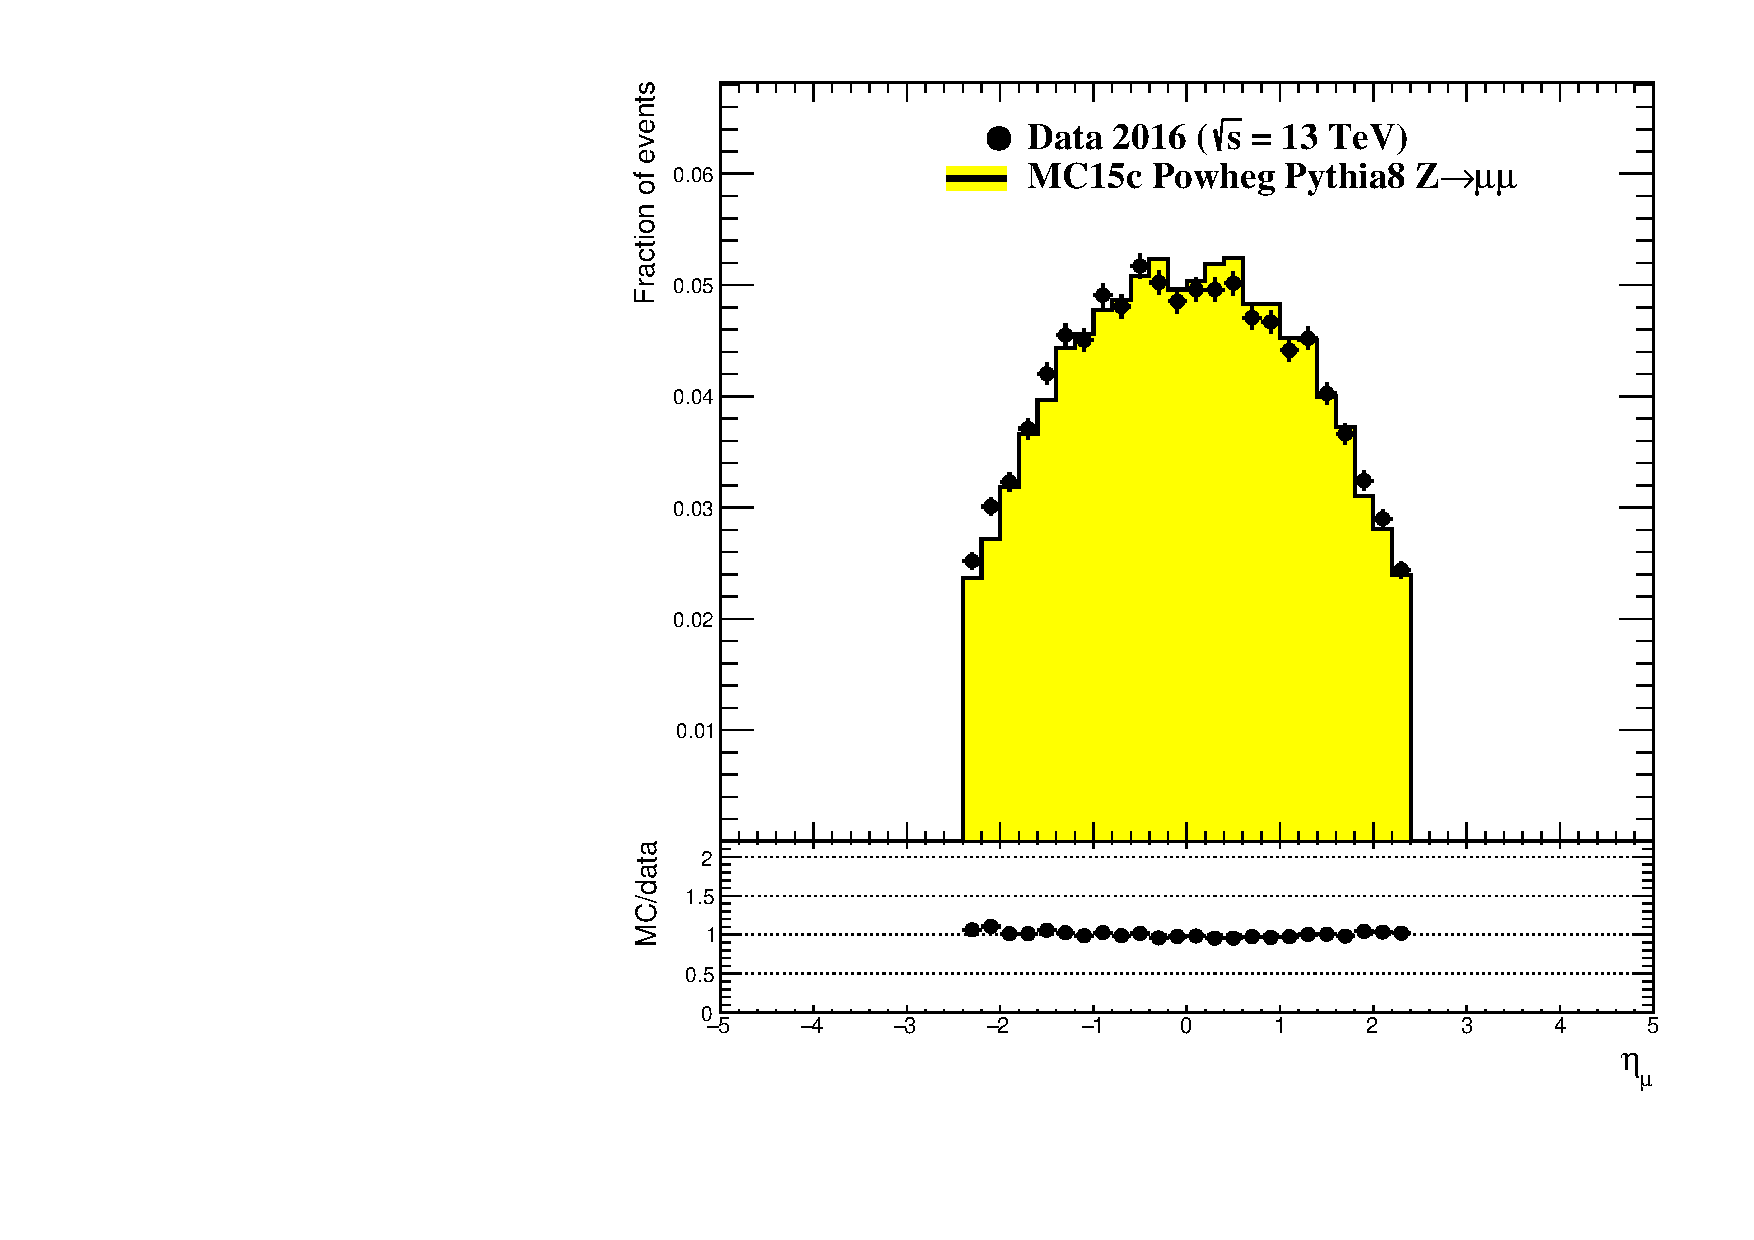
\includegraphics[width=0.53\figwidth]{muon_etaratio}
\caption[$\eta$ of the muons]{$\eta_{\mu}$}
\label{fig:muoneta}
\end{subfigure}
\quad
\begin{subfigure}[b]{0.5\figwidth}
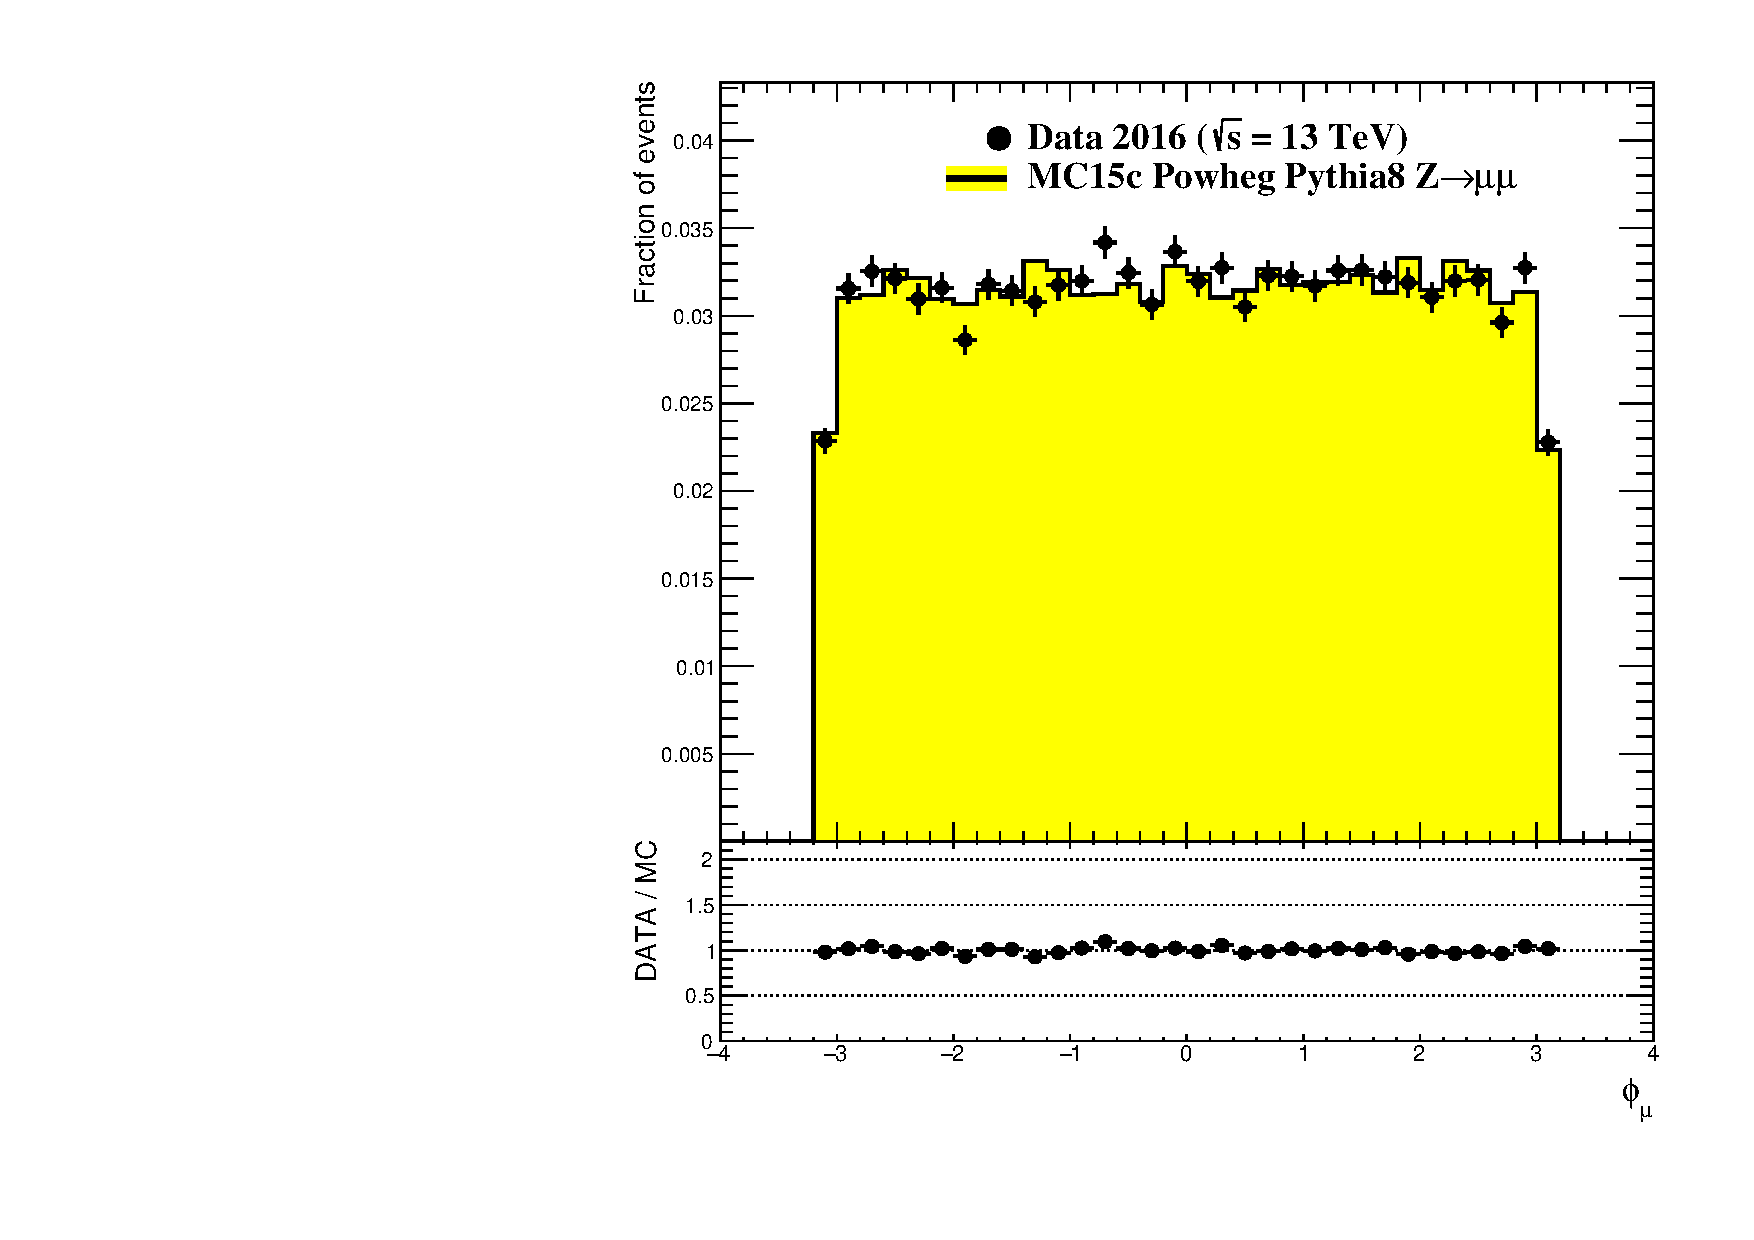
\includegraphics[width=0.53\figwidth]{muon_phiratio}
\caption[$\phi$ of the muons]{$\phi_{\mu}$}
\label{fig:muonphi}
\end{subfigure}
\caption{Properties of the two muons. The histograms are normalized. The distributions shown are: \ref{fig:muonpt} the transversal momentum of the muons; \ref{fig:muone} the muons' energy; \ref{fig:muoneta} the muons' $\eta$ and \ref{fig:muonphi} the muons' $\phi$}
\label{fig:muons}
\end{figure}


\begin{figure}[h]
\centering
\begin{subfigure}[b]{0.5\figwidth}
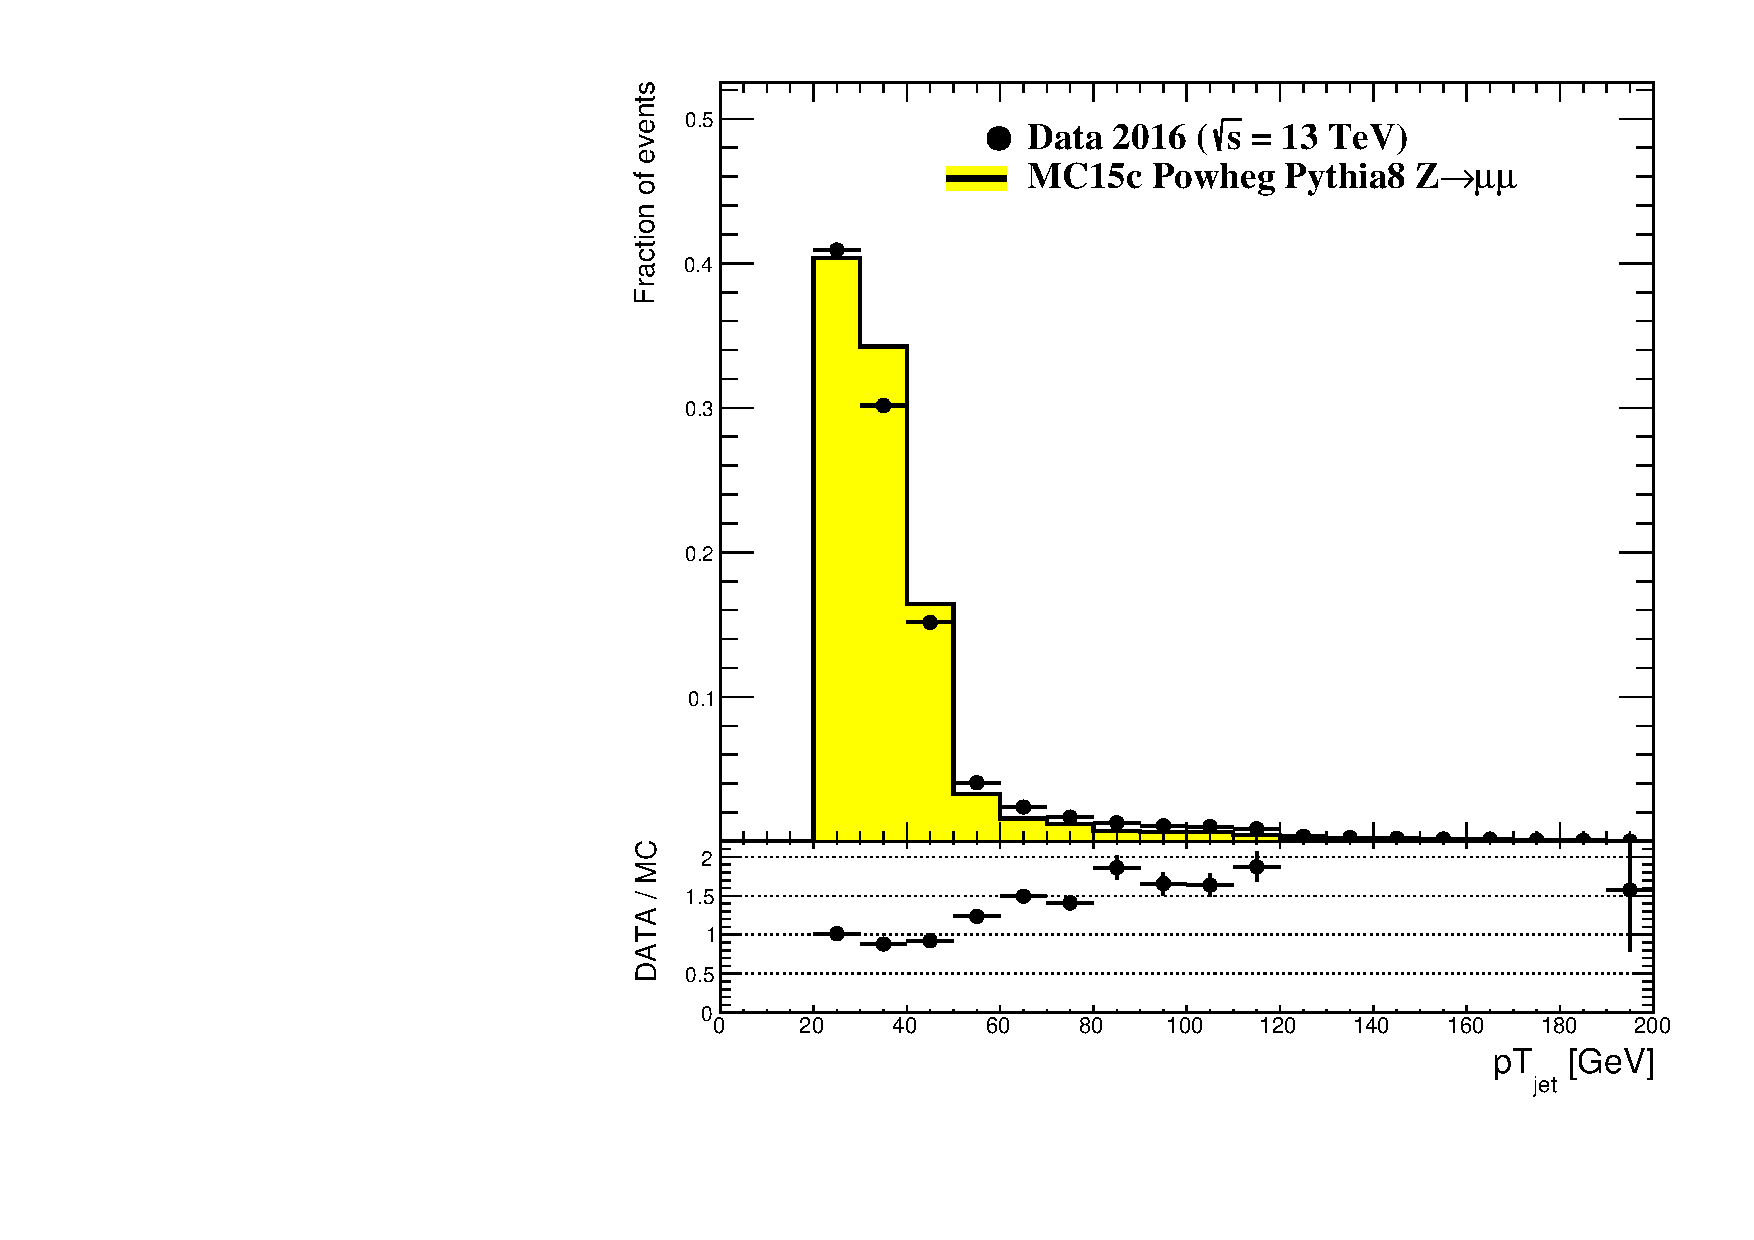
\includegraphics[width=0.53\figwidth]{jet_ptratio}
\caption[Transversal momentum of the recoiling jet]{$pT_{jet}$}
\label{fig:jetpt}
\end{subfigure}
\quad
\begin{subfigure}[b]{0.5\figwidth}
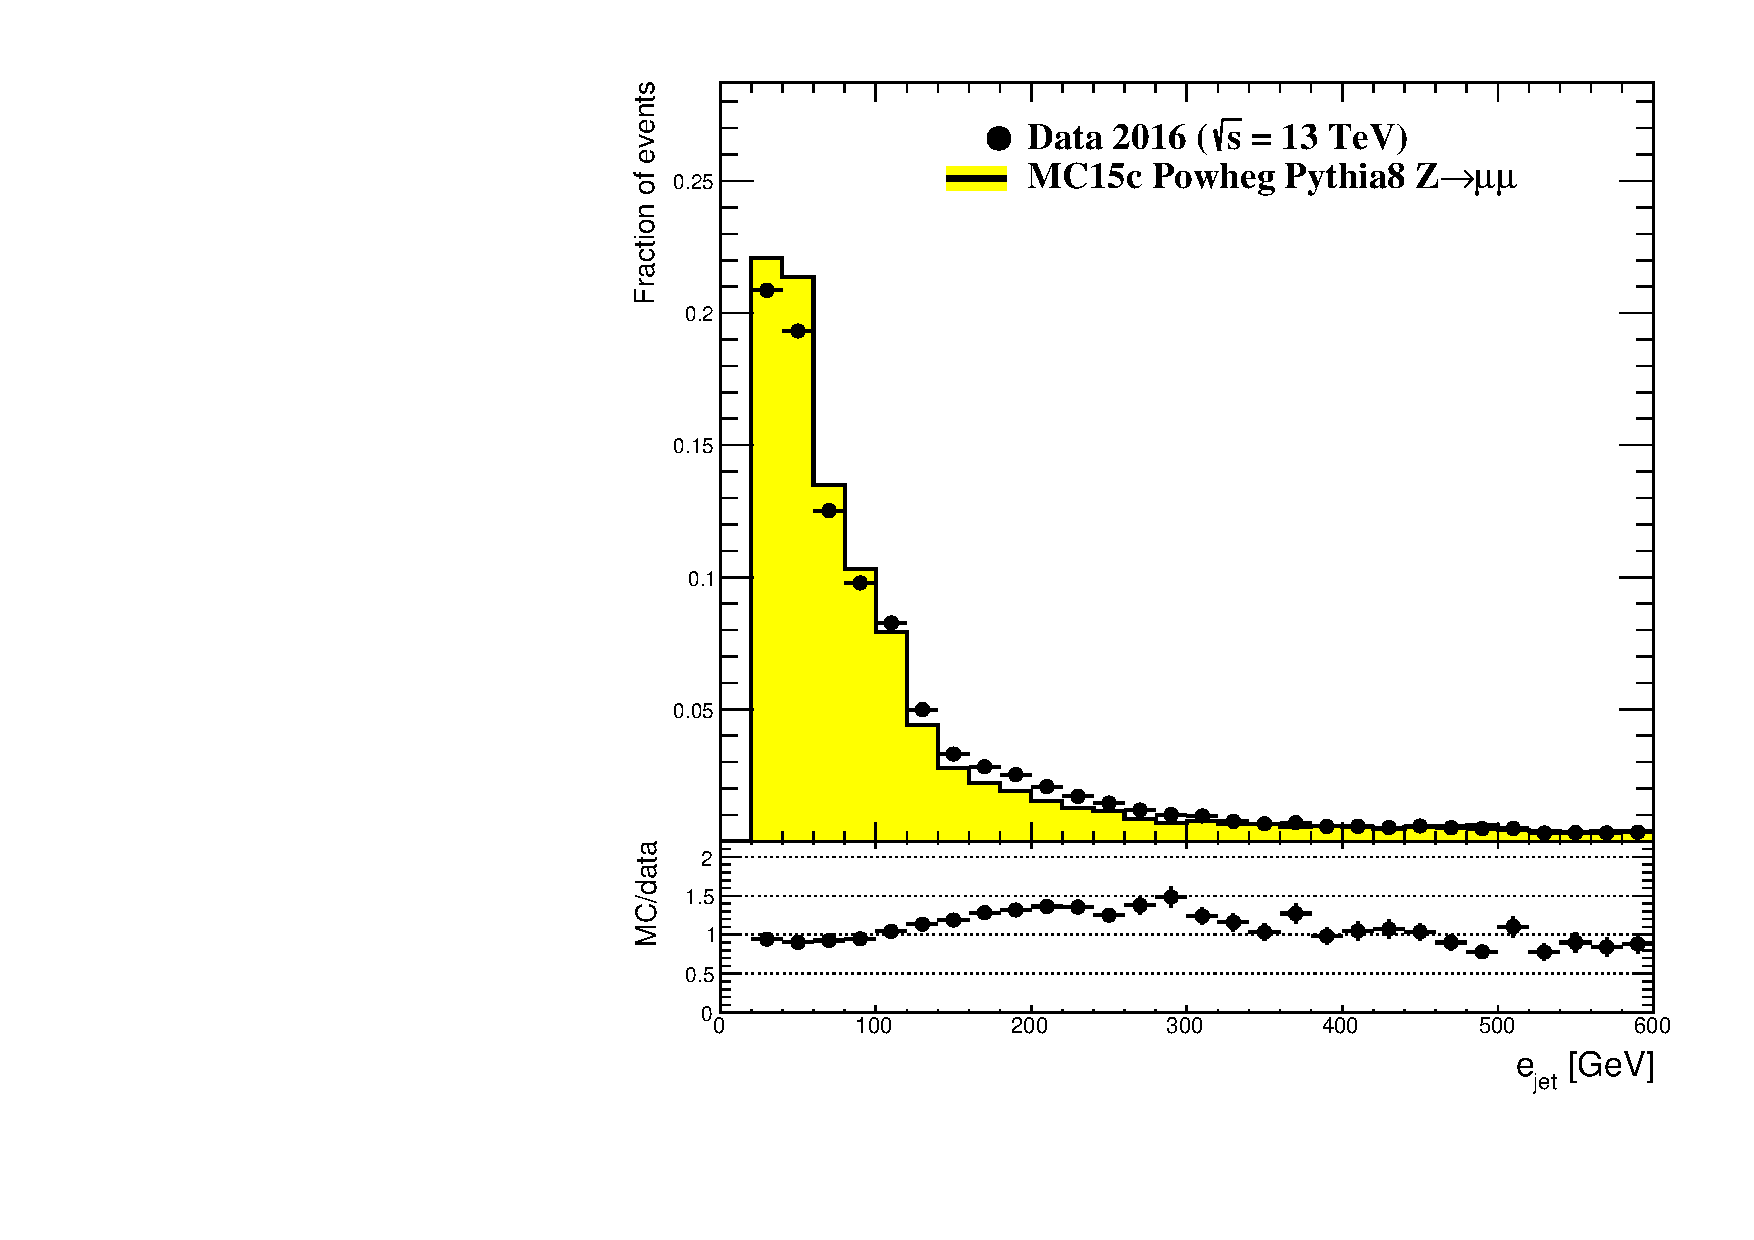
\includegraphics[width=0.53\figwidth]{jet_eratio}
\caption[Energy of the recoiling jet]{$e_{jet}$}
\label{fig:jete}
\end{subfigure}
\end{figure}


\begin{figure}[h]
\centering
\begin{subfigure}[b]{0.5\figwidth}
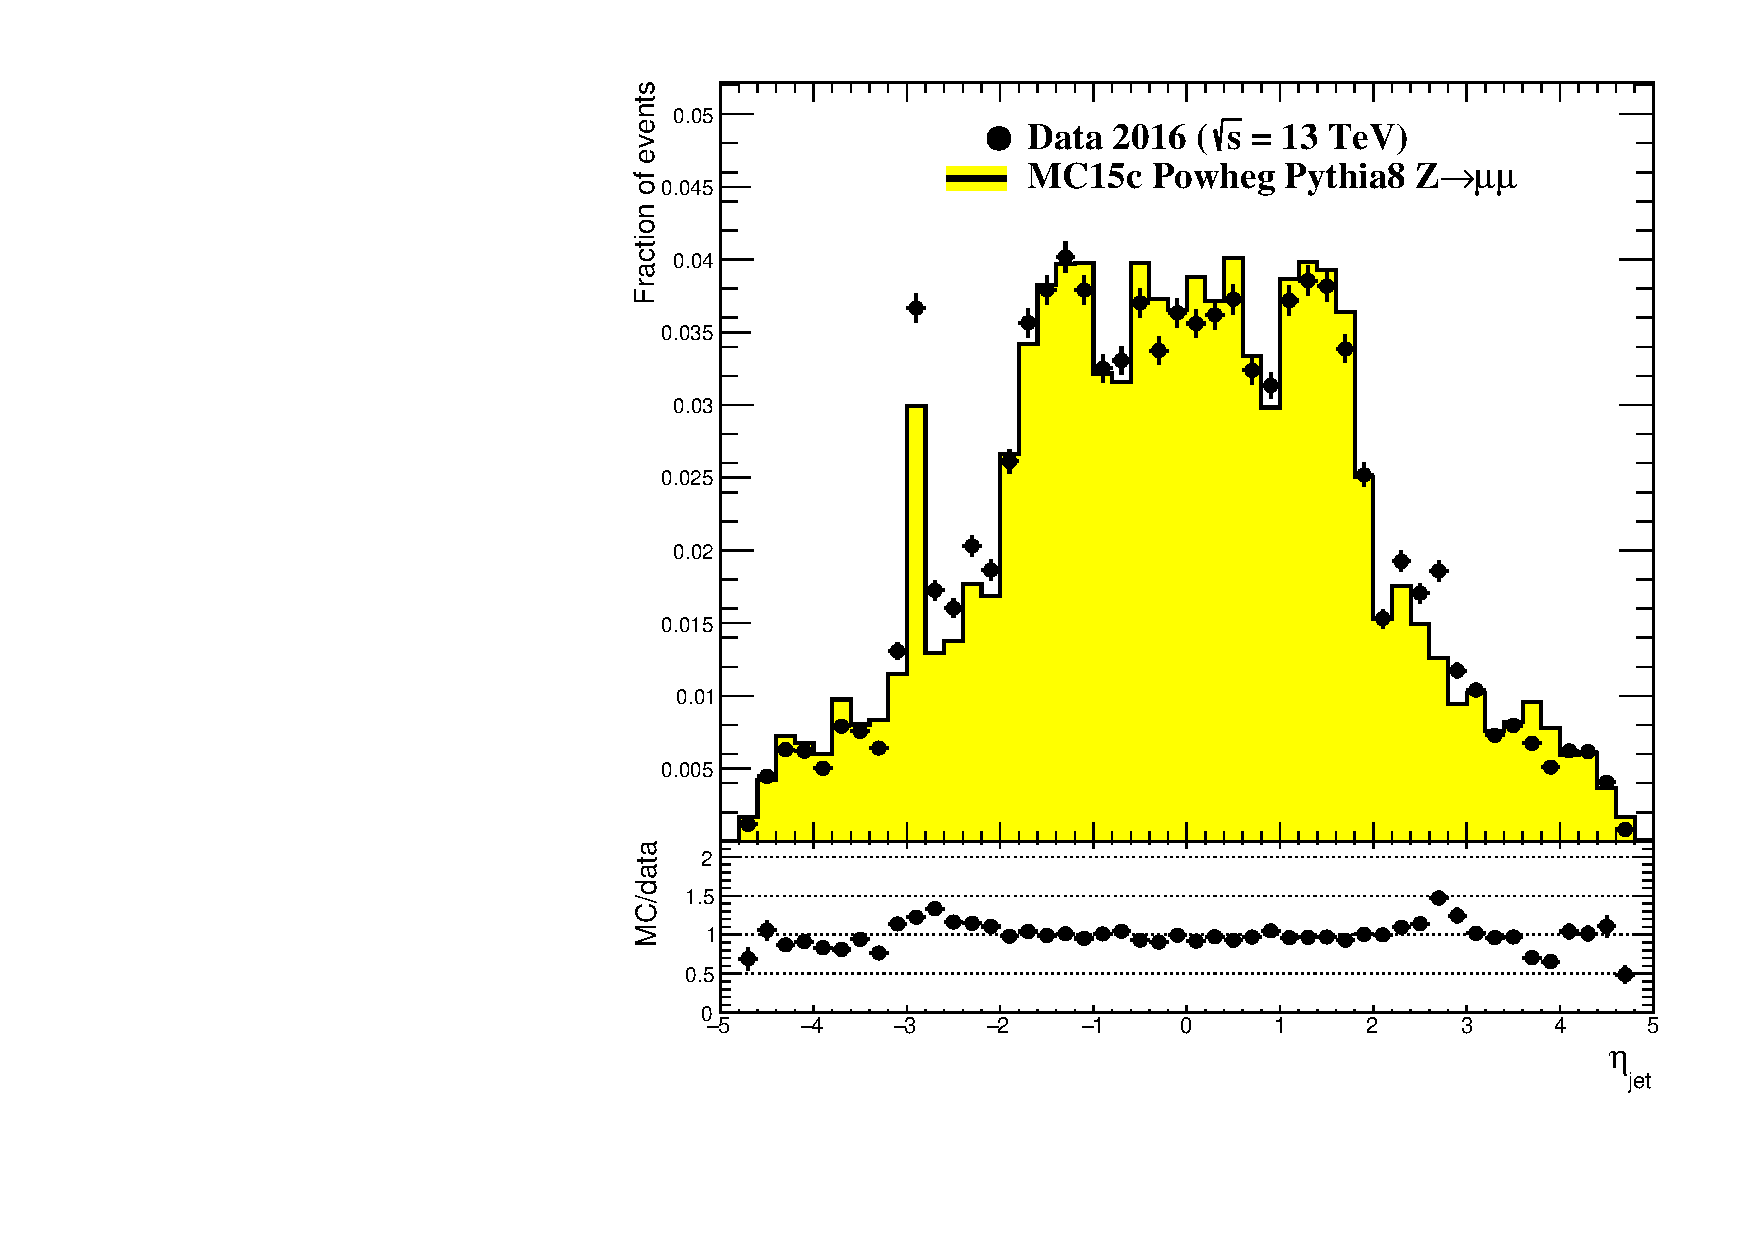
\includegraphics[width=0.53\figwidth]{jet_etaratio}
\caption[$\eta$ of the recoiling jet]{$\eta_{jet}$}
\label{fig:jeteta}
\end{subfigure}
\quad
\begin{subfigure}[b]{0.5\figwidth}
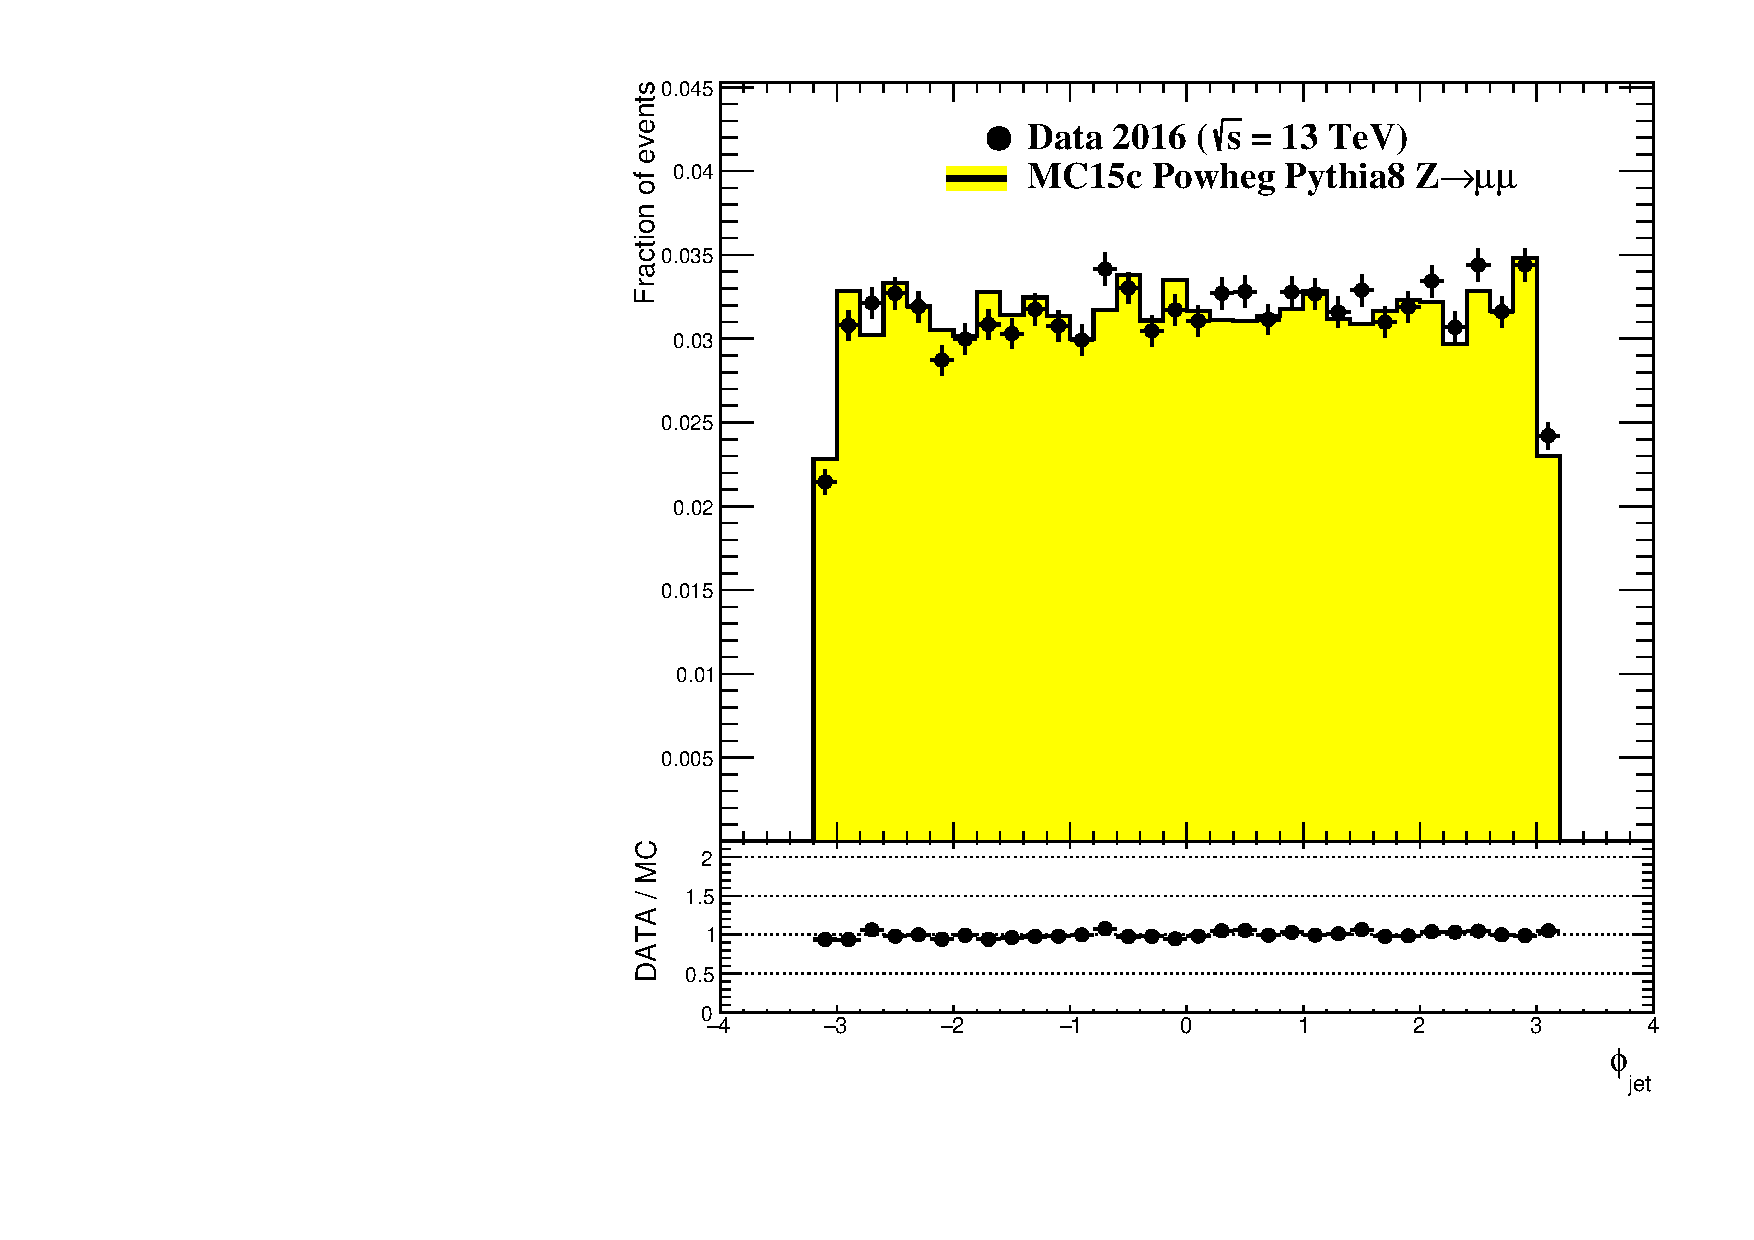
\includegraphics[width=0.53\figwidth]{jet_phiratio}
\caption[$\phi$ of the recoiling jet]{$\phi_{jet}$}
\label{fig:jetphi}
\end{subfigure}
\caption{Properties of the recoiling jet. The distributions are normalized to the number of jets. Distributions shown are: \ref{fig:jetpt} the jet's transversal momentum; \ref{fig:jete} the jet's energy; \ref{fig:jeteta} the jet's eta and \ref{fig:jetphi} the jet's phi.}
\label{fig:reoilingjet}
\end{figure}

\section{Reconstruction of the Z-Boson}

The $Z-Boson$ is reconstructed as the vector-sum of the two muons in the selected event.
It is required to be in an range of \SI{90+-10}{\GeV} and to have a transversal momentum greater than \SI{30}{\GeV}.

Figure \ref{fig:z} shows the properties of the reconstructed $Z$-Boson in data/MC comparison. The agreement of data and Monte Carlo for the $Z$ is in general very good. The momentum resolution worsens slightly with $pT$ exceeding $\SI{80}{\GeV}$ but keeps a reasonable value. The mass of the $Z-Boson$ fluctuates in a range of about \SI{5}{\GeV} around the expected value of \SI{91.19}{\GeV} and has a good agreement with the MC.
The angular agreement is also very good.


\begin{figure}[h]
\centering
\begin{subfigure}[b]{0.5\figwidth}
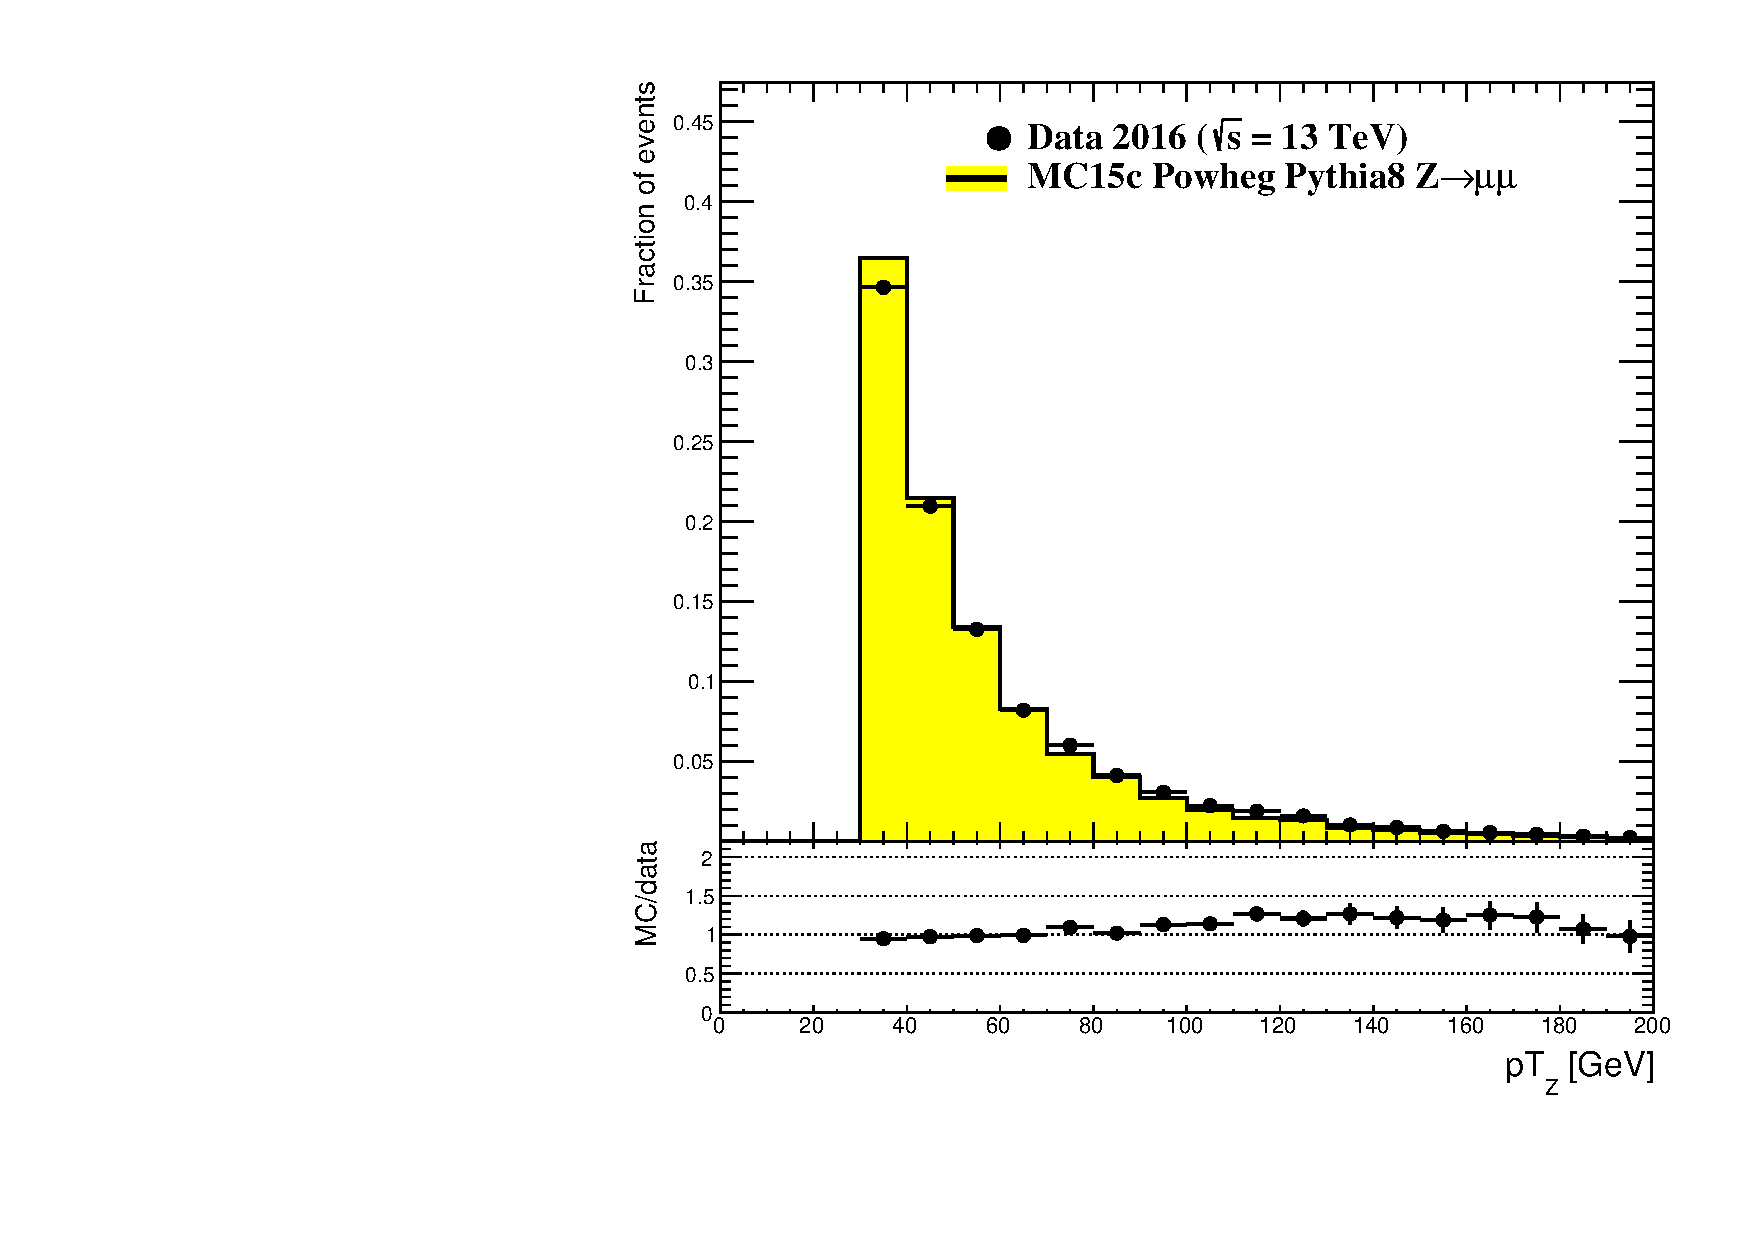
\includegraphics[width=0.53\figwidth]{Z_ptratio}
\caption[Transversal momentum of the reconstructed Z]{$pT_Z$}
\label{fig:zpt}
\end{subfigure}
\quad
\begin{subfigure}[b]{0.5\figwidth}
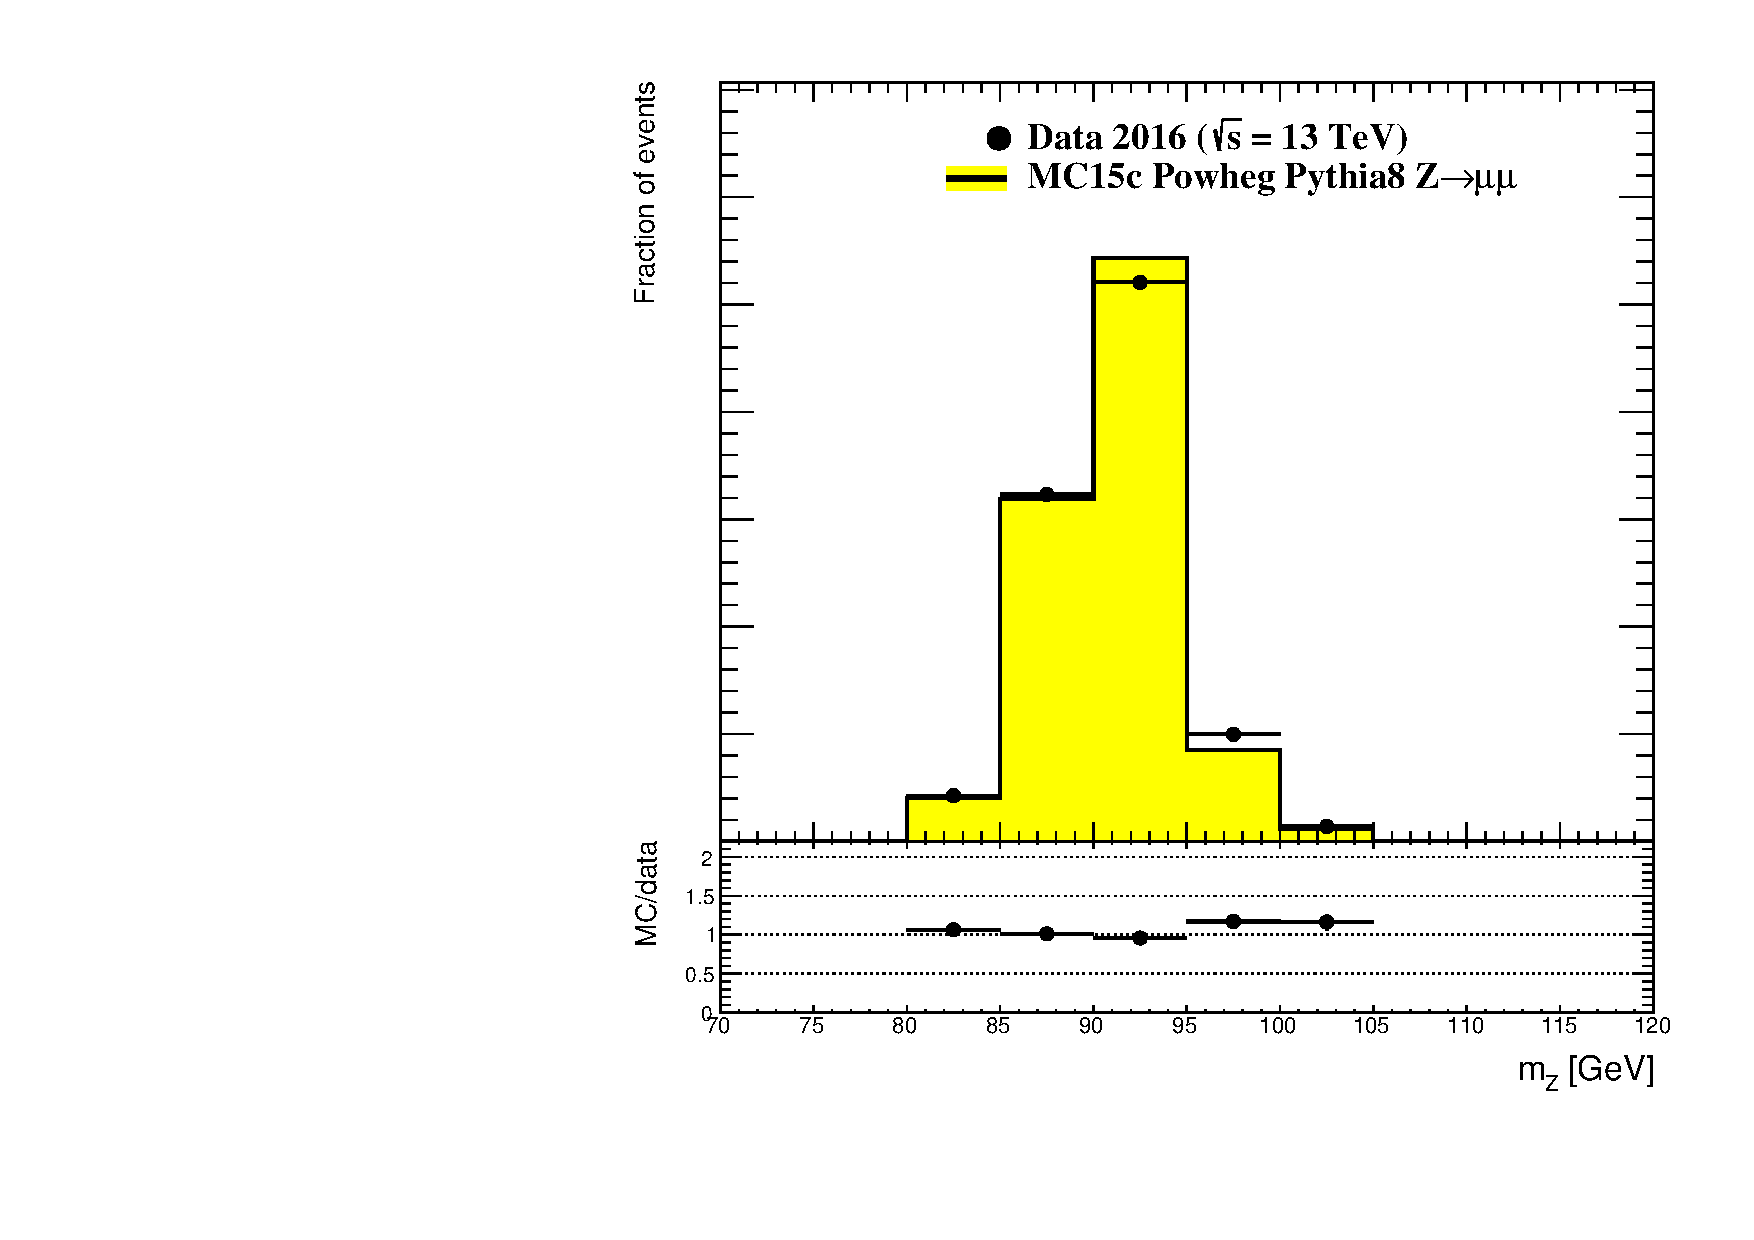
\includegraphics[width=0.53\figwidth]{Z_mratio}
\caption[mass of the reconstructed $Z$]{$m_Z$}
\label{fig:zm}
\end{subfigure}
\end{figure}


\begin{figure}[h]
\centering
\begin{subfigure}[b]{0.5\figwidth}
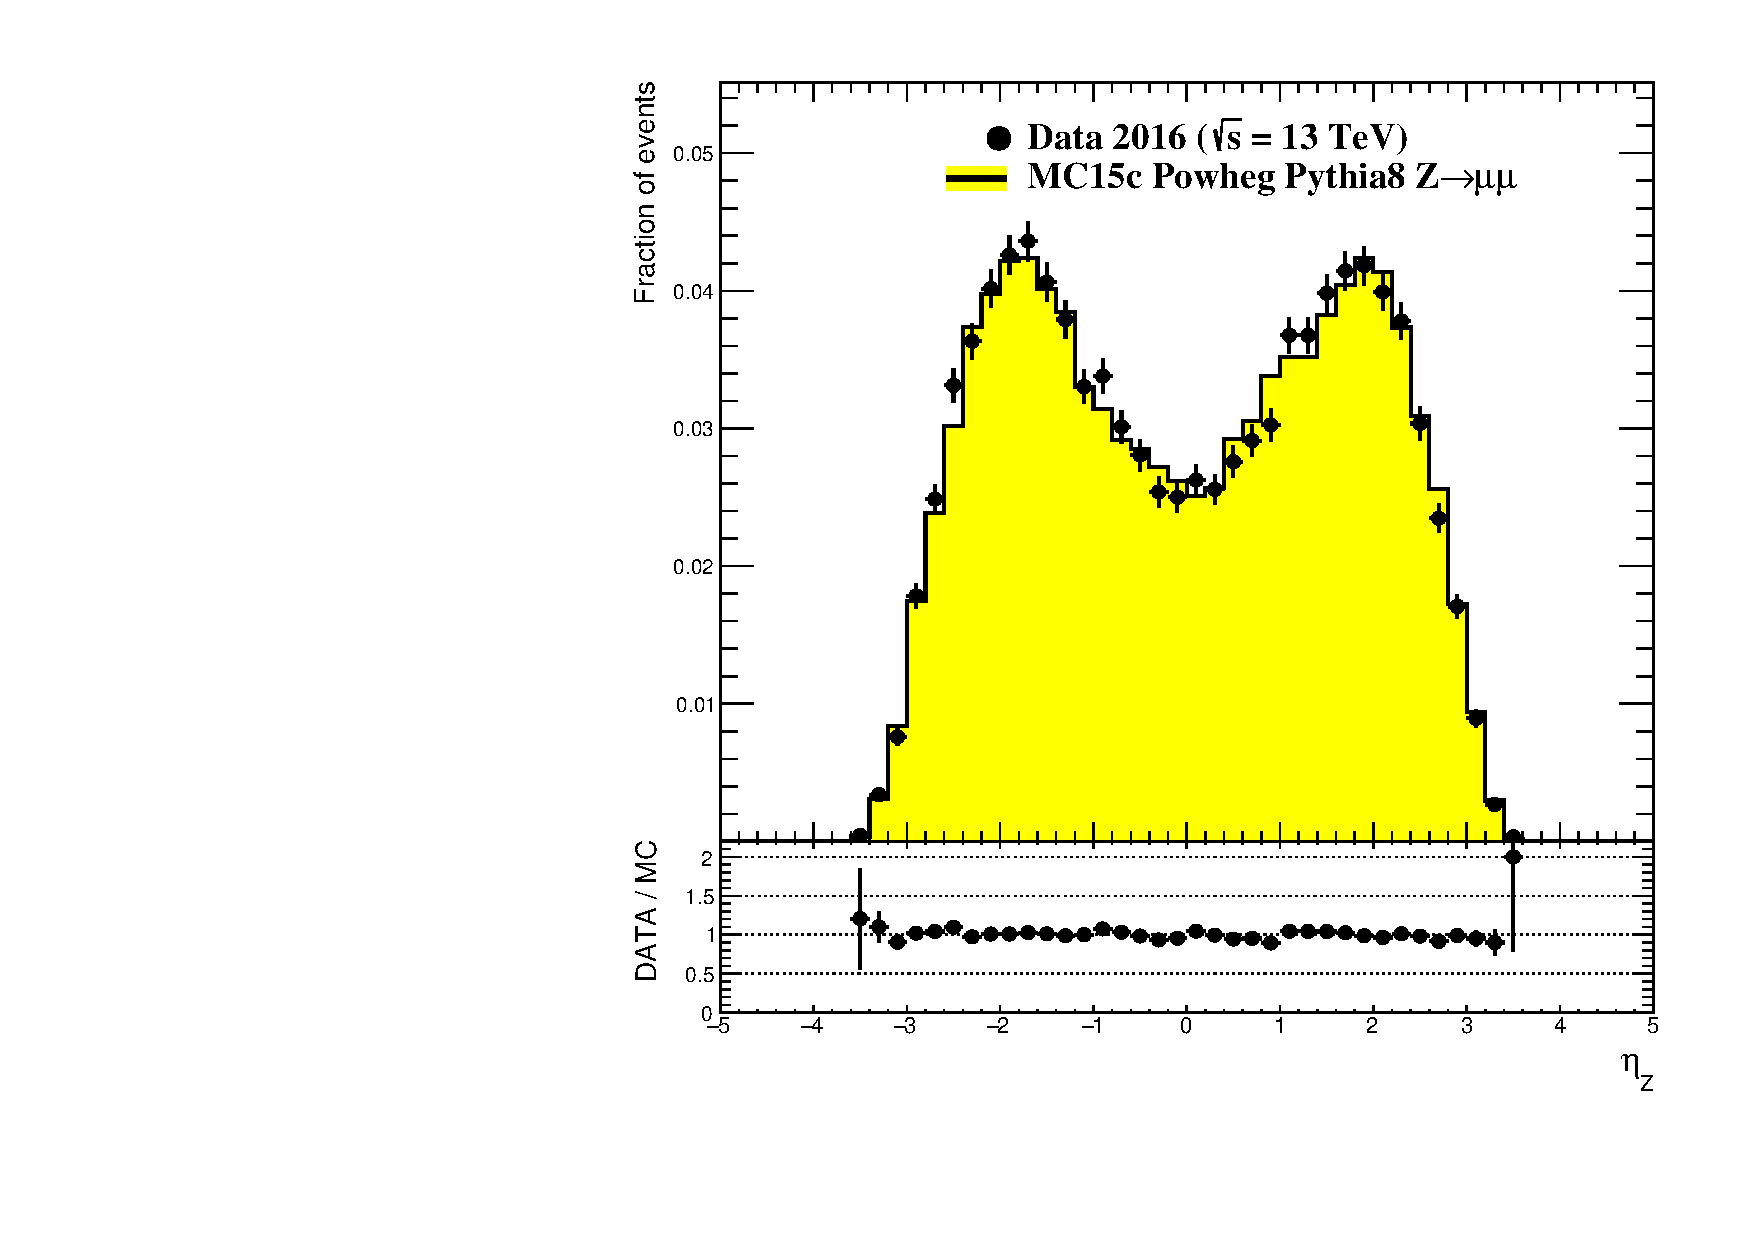
\includegraphics[width=0.53\figwidth]{Z_etaratio}
\caption[$\eta$ of the reconstructed $Z$]{$\eta_Z$}
\label{fig:zeta}
\end{subfigure}
\quad
\begin{subfigure}[b]{0.5\figwidth}
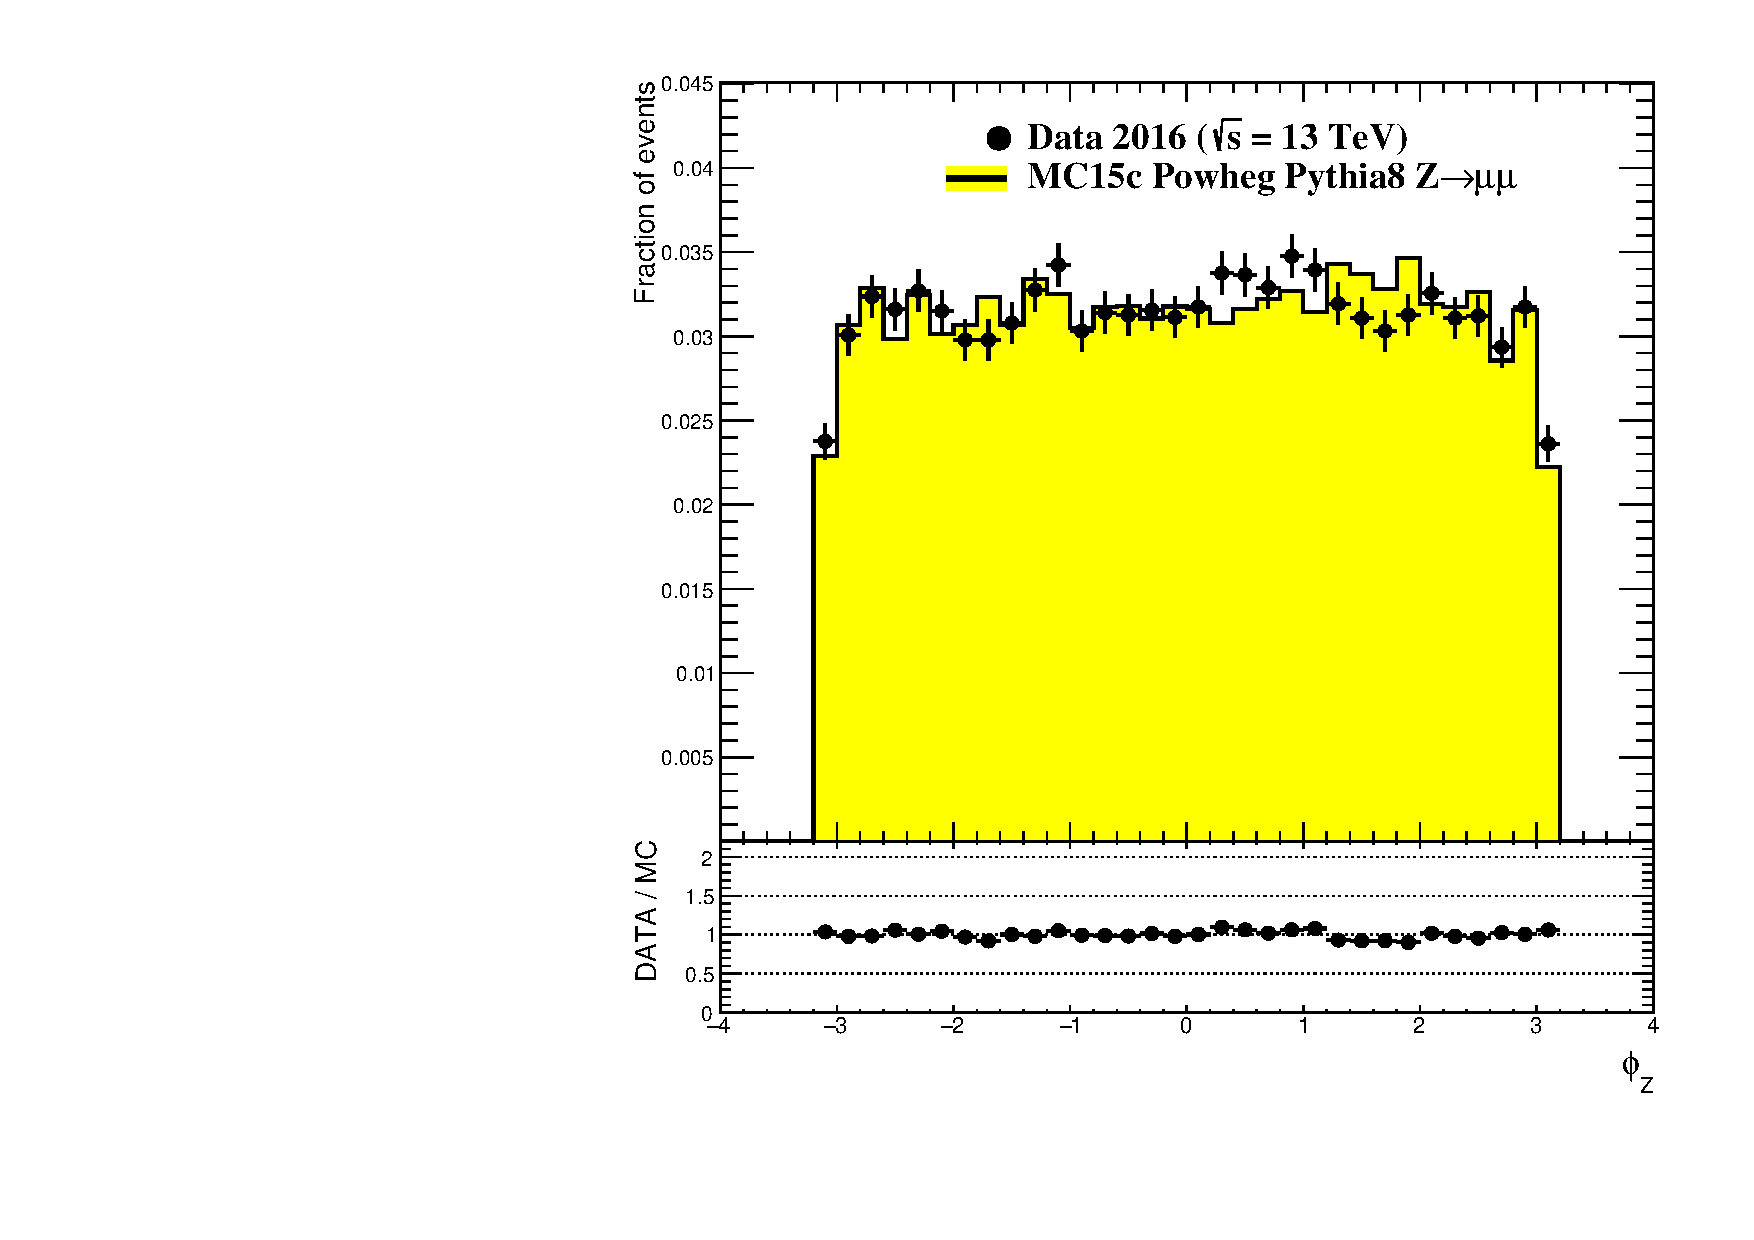
\includegraphics[width=0.53\figwidth]{Z_phiratio}
\caption[$\phi$ of the reconstructed $Z$]{$\phi_Z$}
\label{fig:zphi}
\end{subfigure}
\caption{Properties of the reconstructed Z-Boson. MC and data are normalized. The distributions show \ref{fig:zpt} the transversal momentum; \ref{fig:zm} the mass; \ref{fig:zeta} the pseudorapidity and \ref{fig:zphi} the $\phi$ of the $Z$.}
\label{fig:z}
\end{figure}



\section{Performance of general variables}


This sections shows the comparison of data and Monte Carlo for some further jet and event variables displayed in figure \ref{fig:generalproperties}.

The first distribution shows the number of vertices per event. The agreement between data and MC is rather bad. The center of the MC-distribution is displaced to the left with respect to the data distribution. This suggests that the MC needs further weighting to match the data better. Given that the completion of the weighting is still in process one can hope that a proper weighting of the vertices might also improve other distributions. Nevertheless the distributions for data and MC are comparable and show similar shapes.

The second distribution \ref{fig:chfrac} shows the fraction of jet-$pT$ carried by reconstructed tracks. The agreement is decent although a weighting in MC might optimize it still. The first bin here is not an overflow bin but refers to neutral objects.

The third distribution \ref{fig:trackcount} shows the number of tracks in a jet. The agreement worsens for a high track multiplicity. This might be due to insufficient statistics. Furthermore there might be wrong tracks reconstructed in data because the data multiplicity generally is higher that in MC.

The last distribution \ref{fig:trackwidth} shows the track width. The agreement is reasonable although the fluctuations can hopefully be mediated by further scaling.

\begin{figure}[h]
\centering
\begin{subfigure}[b]{0.5\figwidth}
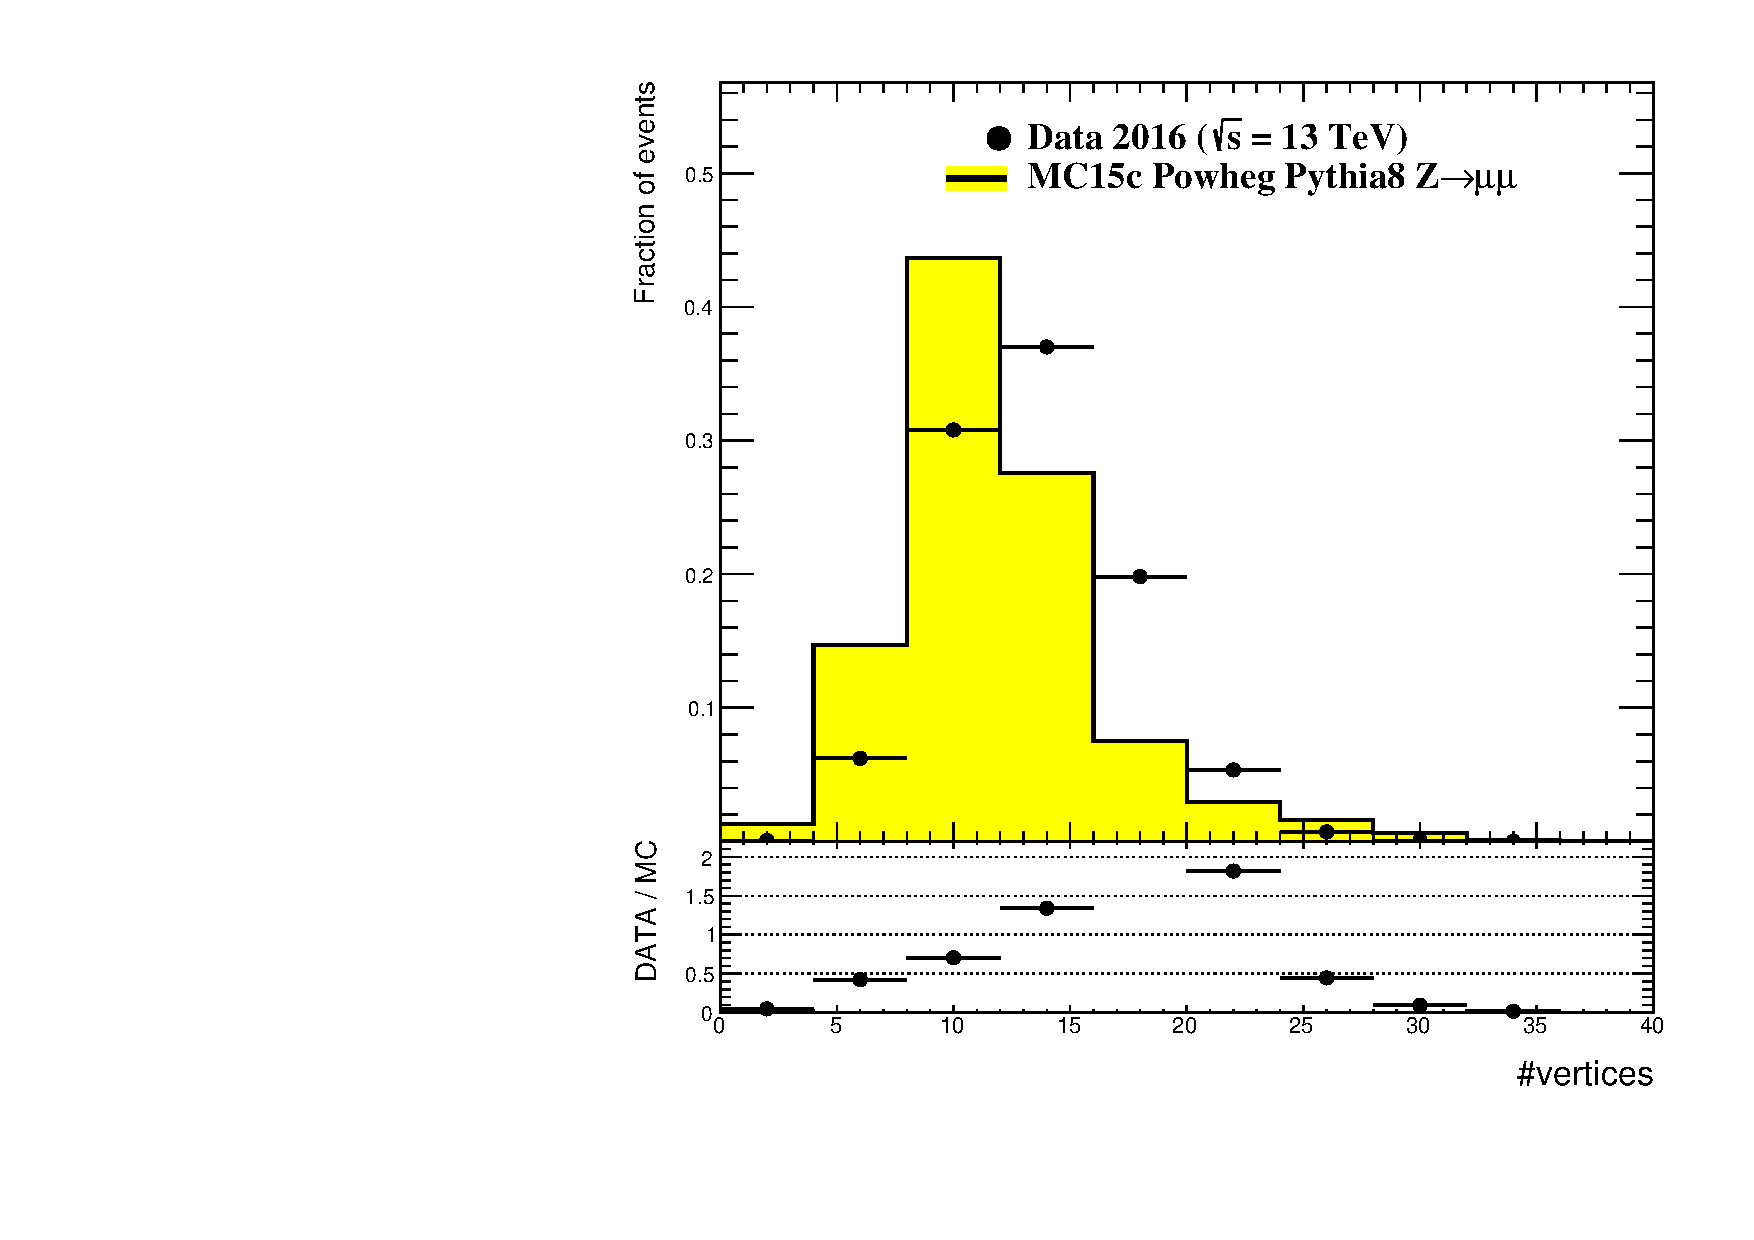
\includegraphics[width=0.53\figwidth]{verticesratio}
\caption[Number of vertices]{Number of vertices}
\label{fig:vertices}
\end{subfigure}
\quad
\begin{subfigure}[b]{0.5\figwidth}
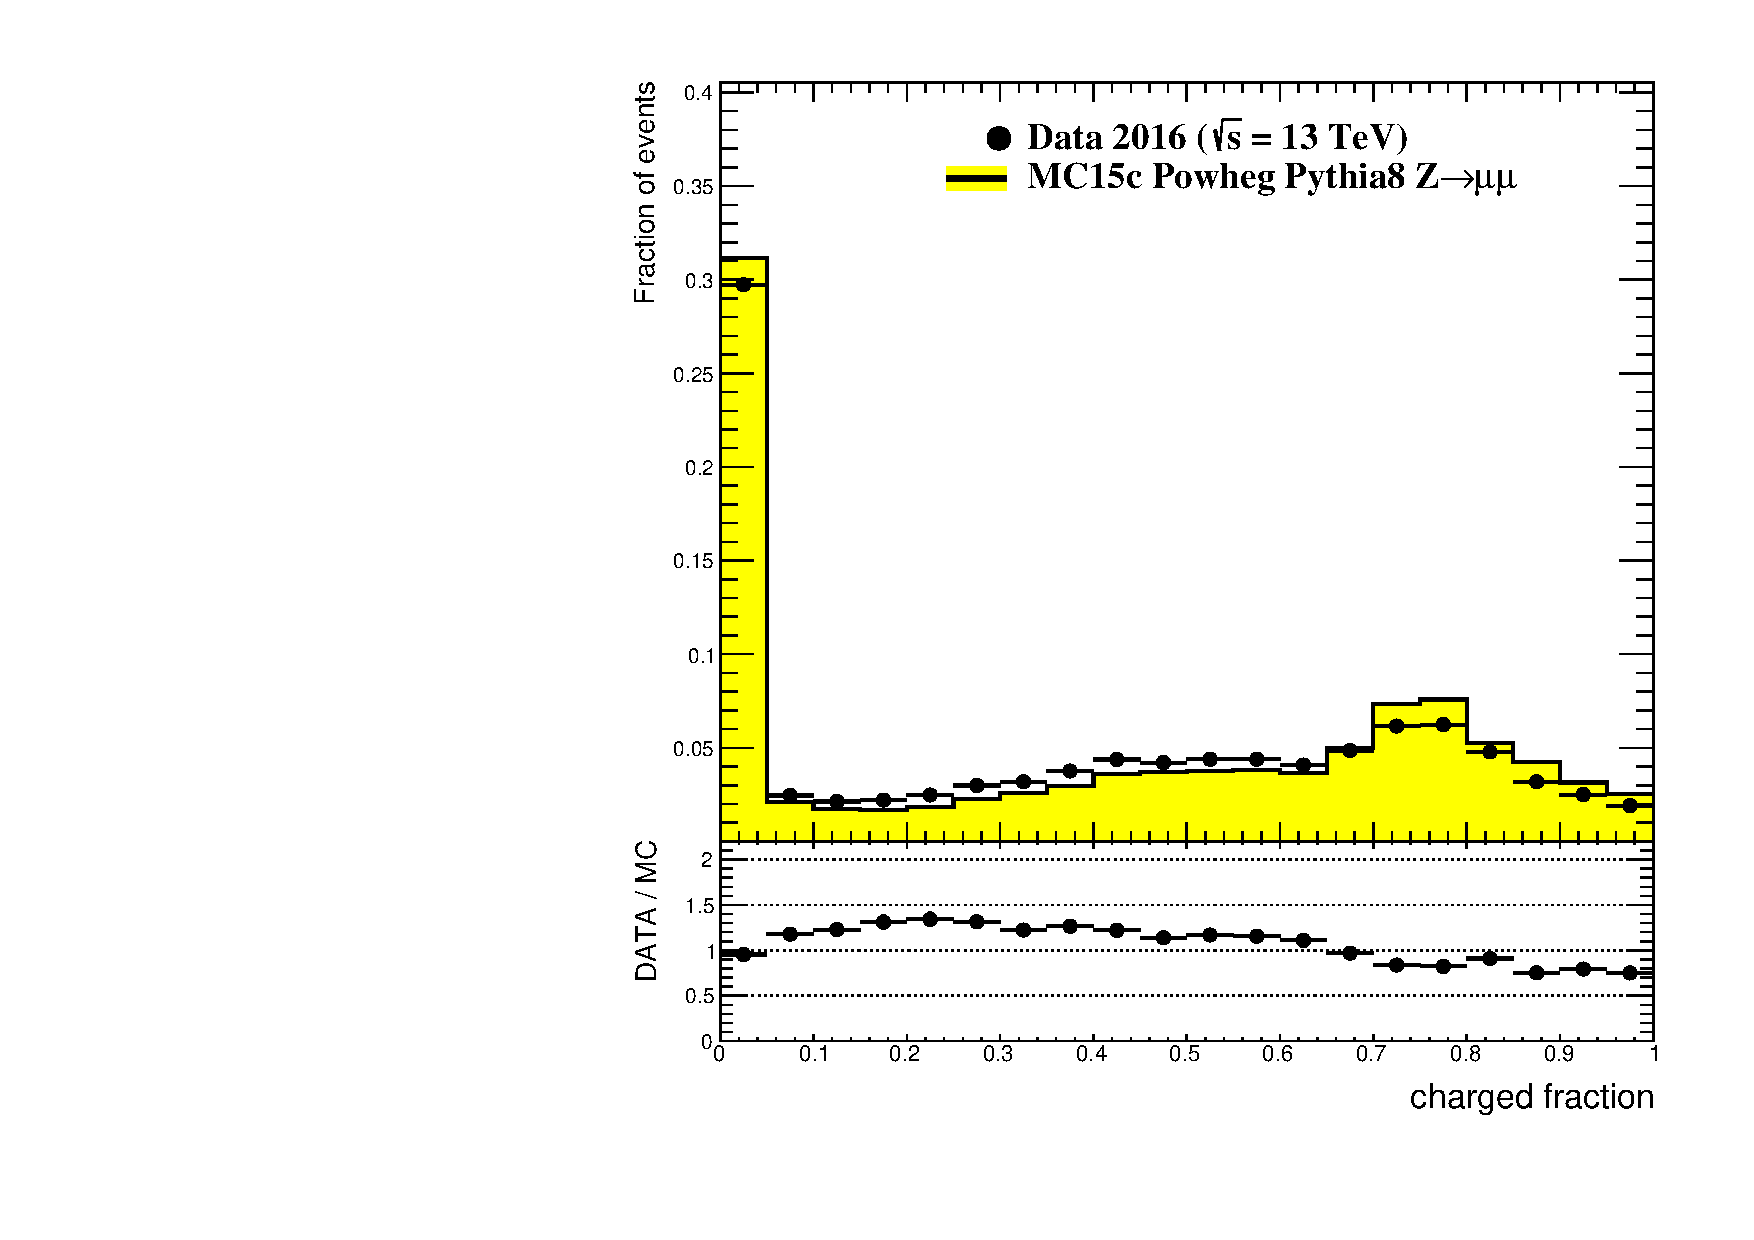
\includegraphics[width=0.53\figwidth]{chfracratio}
\caption[Charged fraction]{Charged fraction}
\label{fig:chfrac}
\end{subfigure}
\end{figure}


\begin{figure}[h]
\centering
\begin{subfigure}[b]{0.5\figwidth}
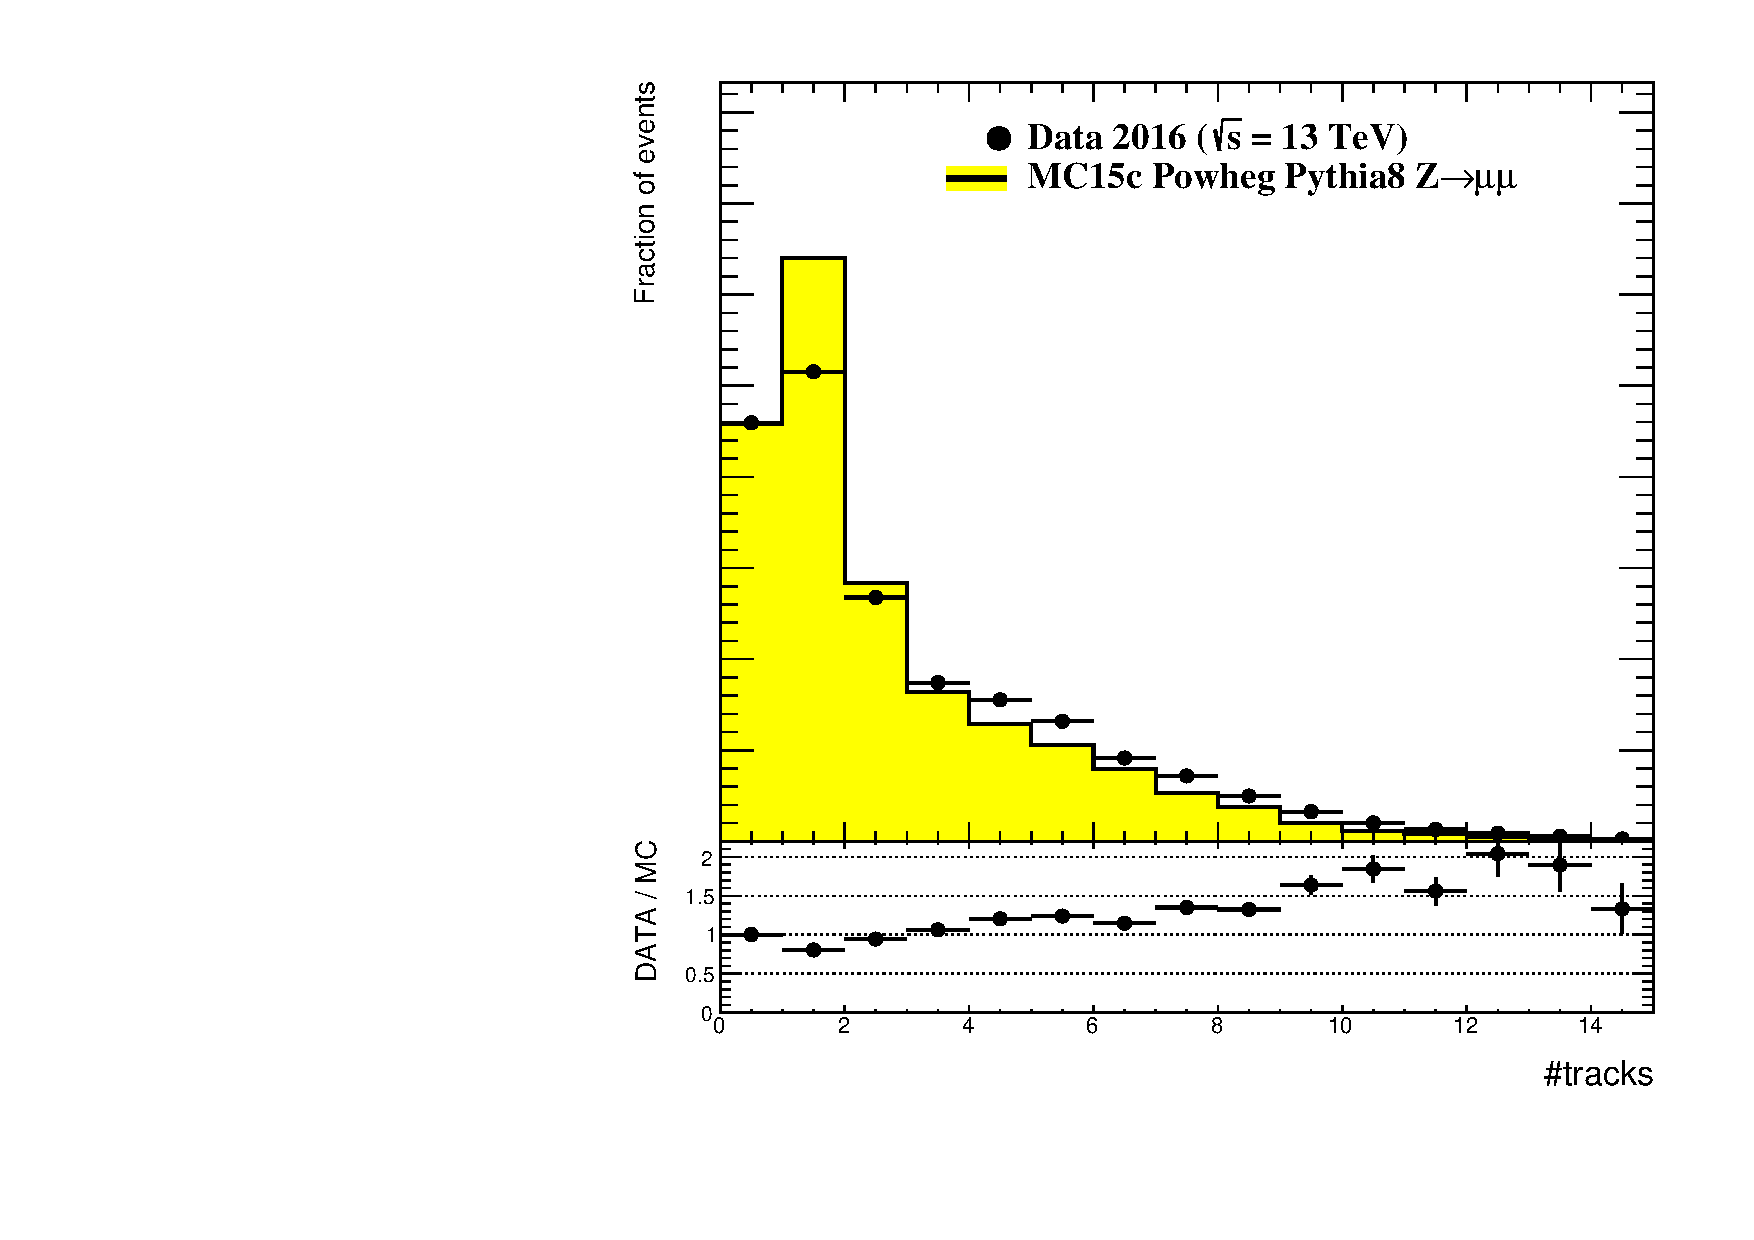
\includegraphics[width=0.53\figwidth]{trackcountratio}
\caption[Track count]{Track count}
\label{fig:trackcount}
\end{subfigure}
\quad
\begin{subfigure}[b]{0.5\figwidth}
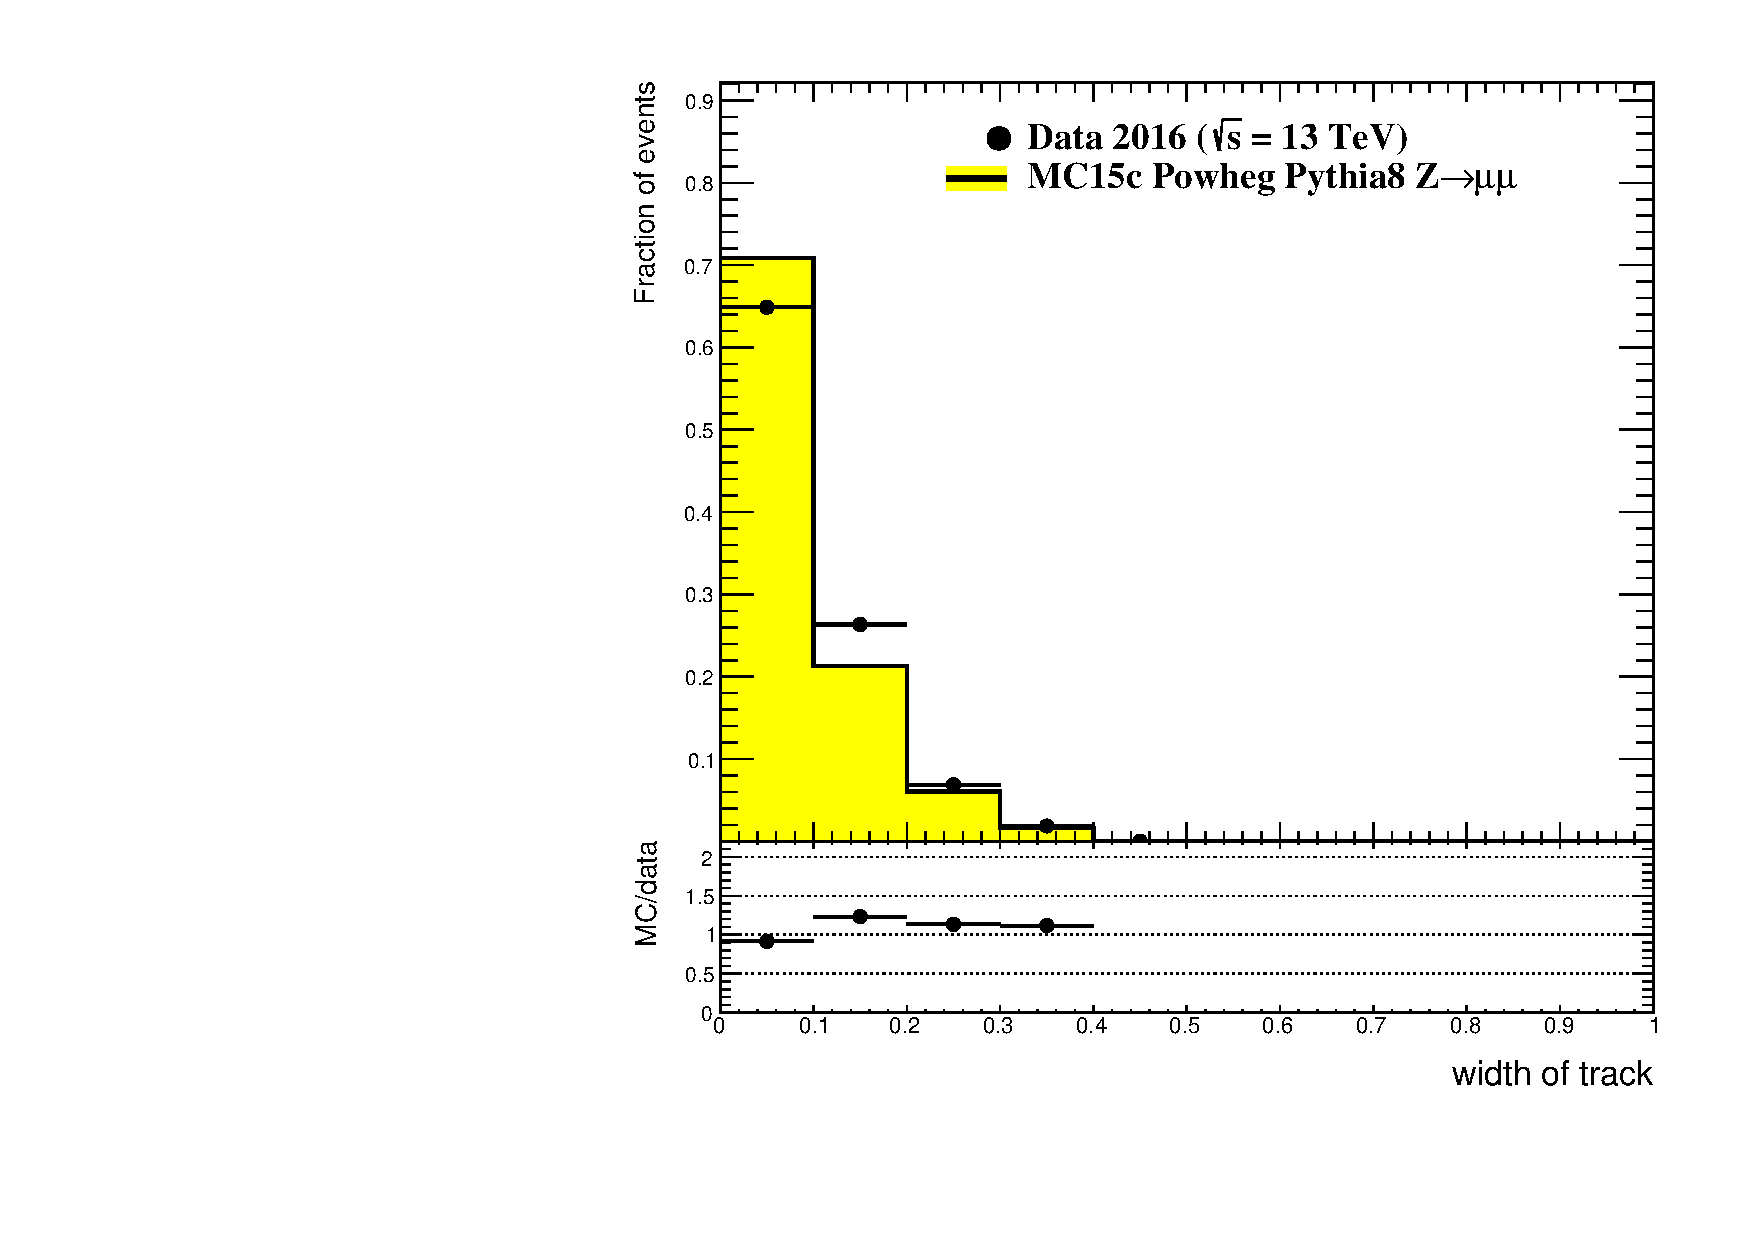
\includegraphics[width=0.53\figwidth]{trackwidthratio}
\caption[trackwidth]{Track width}
\label{fig:trackwidth}
\end{subfigure}
\caption{General event properties in data/MC comparison. The distributions are normalized to the sample size. The following distributions are shown: \ref{fig:vertices} number of vertices in the event; \ref{fig:chfrac} the charged fraction, i.e. the fractional jet $p_T$ carried by reconstructed tracks; \ref{fig:trackcount} the number of tracks in the jet; \ref{fig:trackwidth} the track's width.}
\label{fig:generalproperties}
\end{figure}


\section{Conclusion of the performance}

All things considered the data/MC comparison shows that the Particle Flow framework is on a good way. Right now a full jet calibration as well as jet cleaning for Particle Flow jets is missing. Furthermore the scale factors for all objects and further re-weighting for MC and data have to be applied.
With the improvements expected from these additional tools it is very likely that similar or better results as in Run 1 can be achieves using the Particle Flow algorithm.


\label{results}

% Uncomment the following command to get references per chapter.
% Put it inside the file or change \include to \input if you do not want the references
% on a separate page
% \printbibliography[heading=subbibliography]

%------------------------------------------------------------------------------
% Use biblatex for the bibliography
% Add bibliography to Table of Contents
% Comment out this command if your references are printed for each chapter.
\printbibliography[heading=bibintoc]

%------------------------------------------------------------------------------
% Include the following lines and comment out \printbibliography if
% you use BiBTeX for the bibliography.
% If you use biblatex package the files should be specified in the preamble.
% \KOMAoptions{toc=bibliography}
% {\raggedright
%   \bibliographystyle{../refs/atlasBibStyleWithTitle.bst}
%   % \bibliographystyle{unsrt}
%   \bibliography{./thesis_refs,../refs/standard_refs-bibtex}
% }

%------------------------------------------------------------------------------
\appendix
% \part*{Appendix}
% Add your appendices here - don't forget to also add them to \includeonly above
%------------------------------------------------------------------------------
\chapter{Useful information}
\label{sec:app}
%------------------------------------------------------------------------------

In the appendix you usually include extra information that should be
documented in your thesis, but not interrupt the flow.

%%% Local Variables: 
%%% mode: latex
%%% TeX-master: "../mythesis"
%%% End: 

% \printbibliography[heading=subbibliography]

%------------------------------------------------------------------------------
% Declare lists of figures and tables and acknowledgements as backmatter
% Chapter/section numbers are turned off
\backmatter

\listoffigures
\listoftables

%------------------------------------------------------------------------------
% Print the glossary and list of acronyms
% \printglossaries

%------------------------------------------------------------------------------
% You could instead add your acknowledgements here - don't forget to
% also add them to \includeonly above
% %------------------------------------------------------------------------------
\chapter*{Acknowledgements}
\label{sec:ack}
%------------------------------------------------------------------------------

I would like to thank ...

You should probably use \texttt{\textbackslash chapter*} for
acknowledgements at the beginning of a thesis and
\texttt{\textbackslash chapter} for the end.

%%% Local Variables: 
%%% mode: latex
%%% TeX-master: "../mythesis"
%%% End: 


%------------------------------------------------------------------------------
% CV needed when you submit your PhD thesis
% \definecolor{lightgray}{gray}{0.8}
\newcolumntype{L}{>{\raggedleft}p{0.15\textwidth}}
\newcolumntype{R}{p{0.8\textwidth}}
\newcommand\VRule{\color{lightgray}\vrule width 0.5pt}

\thispagestyle{empty}
\section*{Curriculum Vitae}

\subsection*{Personal Details}

\begin{tabular}{L!{\VRule}R}
Name & Johann Schmidt \\
Date of Birth &  \\
Email & abc@physik.uni-def.de \\
Family status & Single
\end{tabular}

\subsection*{Education}

\begin{tabular}{L!{\VRule}R}
1997--2003 & Abitur, ABC Secondary School, Hamburg, Germany\\
2004--2007 & BSc in Physics, Rheinische Friedrich-Wilhelms-Universität, Bonn, Germany.\\
2006 & CERN Summer Student, Geneva, Switzerland. \\
2007--2009 &  MSc in Physics Rheinische Friedrich-Wilhelms-Universität, Bonn, Germany. \\
2009--2012 &  PhD in Physics, Rheinische Friedrich-Wilhelms-Universität, Bonn, Germany. \\
2012 & Advanced Data Analysis School, Frankfurt, Germany.
\end{tabular}

\subsection*{Professional Experience}

\begin{tabular}{L!{\VRule}R}
2004 & Summer Student at CERN, Geneva, Switzerland. \\
2007--2012 & Doctoral work at the University of Bonn, Germany. \\
2008--2009 & Fieldwork at CERN, Geneva, Switzerland.\\
2011 & Talk at the Advanced Physics Conference, Timbucto
\end{tabular}

\subsection*{Languages}
\begin{tabular}{L!{\VRule}R}
German & Mother tongue \\
English & Fluent \\
Russian & Basic
\end{tabular}


\end{document}

%%% Local Variables:
%%% mode: latex
%%% TeX-master: t
%%% End:
